%
% Niniejszy plik stanowi przykład formatowania pracy magisterskiej na
% Wydziale MIM UW.  Szkielet użytych poleceń można wykorzystywać do
% woli, np. formatujac wlasna prace.
%
% Zawartosc merytoryczna stanowi oryginalnosiagniecie
% naukowosciowe Marcina Wolinskiego.  Wszelkie prawa zastrzeżone.
%
% Copyright (c) 2001 by Marcin Woliński <M.Wolinski@gust.org.pl>
% Poprawki spowodowane zmianami przepisów - Marcin Szczuka, 1.10.2004
% Poprawki spowodowane zmianami przepisow i ujednolicenie 
% - Seweryn Karłowicz, 05.05.2006
% Dodanie wielu autorów i tłumaczenia na angielski - Kuba Pochrybniak, 29.11.2016

% dodaj opcję [licencjacka] dla pracy licencjackiej
% dodaj opcję [en] dla wersji angielskiej (mogą być obie: [licencjacka,en])
\documentclass[en]{pracamgr}

% Dane magistranta:
\autor{Wiktor Grzankowski}{429211}

\title{Stable Priceability for Additive Utilities}
\titlepl{Pojęcie Stable Priceability dla addytywnych użyteczności}

%\tytulang{An implementation of a difference blabalizer based on the theory of $\sigma$ -- $\rho$ phetors}

%kierunek: 
% - matematyka, informacyka, ...
% - Mathematics, Computer Science, ...
\kierunek{Computer Science}

% informatyka - nie okreslamy zakresu (opcja zakomentowana)
% matematyka - zakres moze pozostac nieokreslony,
% a jesli ma byc okreslony dla pracy mgr,
% to przyjmuje jedna z wartosci:
% {metod matematycznych w finansach}
% {metod matematycznych w ubezpieczeniach}
% {matematyki stosowanej}
% {nauczania matematyki}
% Dla pracy licencjackiej mamy natomiast
% mozliwosc wpisania takiej wartosci zakresu:
% {Jednoczesnych Studiow Ekonomiczno--Matematycznych}

% \zakres{Tu wpisac, jesli trzeba, jedna z opcji podanych wyzej}

% Praca wykonana pod kierunkiem:
% (podać tytuł/stopień imię i nazwisko opiekuna
% Instytut
% ew. Wydział ew. Uczelnia (jeżeli nie MIM UW))
\opiekun{dr hab. Piotr Skowron\\
  Faculty of Mathematics,\\
Informatics and Mechanics\\
  }

% miesiąc i~rok:
\date{September 2025}

%Podać dziedzinę wg klasyfikacji Socrates-Erasmus:
\dziedzina{ 
11.3 Informatyka
}

%Klasyfikacja tematyczna wedlug AMS (matematyka) lub ACM (informatyka)
\klasyfikacja{
\begin{itemize}
    \item Theory of computation
\end{itemize}
}

% Słowa kluczowe:
\keywords{elections, social choice theory, participatory budgeting, priceability, stable-priceability, method of equal shares}


% koniec definicji
\usepackage[utf8]{inputenc} 
\usepackage{polski}
\usepackage{graphicx}
\usepackage{amsmath}
\usepackage{amssymb}
\usepackage{amsfonts}
\usepackage{amsthm}
\usepackage[shortlabels]{enumitem}
\usepackage{mathdots}
\usepackage{url}
\usepackage{xfrac}
\usepackage{array}
\usepackage{hyperref} % referencje do miejsc w pdfie
\usepackage{environ} % zaawansowane środowiska
\usepackage{minted} % formatowanie kodu
\usepackage{tabularx} % lepsze tabelki
\usepackage{wrapfig} % do ustawiania pozycji obrazków
\usepackage{multicol} % wiele kolumn
\usepackage{csquotes}
\usepackage{booktabs}
\usepackage{colortbl}
\usepackage[table]{xcolor}
\usepackage{pifont}
\usepackage[
    backend=biber,
    style=numeric,
    sorting=none,
    urldate=long,
]{biblatex}

% --- Podstawowe matematyczne symbole
\newcommand{\wtw}{\quad \Leftrightarrow \quad}  % wtedy i tylko wtedy
\newcommand{\bigexists}{\mbox{\Large $\mathsurround0pt\exists$}\hspace{0.2em}} 
\newcommand{\bigforall}{\mbox{\Large $\mathsurround0pt\forall$}\hspace{0.1em}}
\newcommand{\lr}[1]{\left\langle #1 \right\rangle}
\renewcommand{\geq}{\geqslant}
\renewcommand{\leq}{\leqslant}

% --- Oznaczenia zbiorów
\newcommand{\RR}{\mathbb{R}}
\newcommand{\ZZ}{\mathbb{Z}}
\newcommand{\NN}{\mathbb{N}}
\newcommand{\CC}{\mathbb{C}}
\newcommand{\KK}{\mathbb{K}}
\newcommand{\QQ}{\mathbb{Q}}

% --- Tekst w math mode
\newcommand{\dm}[1]{\displaystyle{#1}}  % skrót do displaystyle
\newcommand{\textq}[1]{\quad \text{#1} \quad}
\newcommand{\textqq}[1]{\qquad \text{#1} \qquad}

% --- Kolory
\newcommand{\purple}[1]{\textcolor{purple}{#1}}
\newcommand{\teal}[1]{\textcolor{teal}{#1}}
\newcommand{\gray}[1]{\textcolor{gray}{#1}}
\newcommand{\grey}[1]{\textcolor{gray}{#1}}
\newcommand{\red}[1]{\textcolor{red}{#1}}
\newcommand{\orange}[1]{\textcolor{orange}{#1}}

\newcommand{\app}{\ding{51}}  % Approval symbol macro

% --- Kod Pythona
\newminted[python]{python}{
    autogobble,
    mathescape,
    frame = leftline,
    framerule = 1pt,
    framesep = 8pt
}
\newmintinline{python}{}
\addbibresource{bibliography.bib} 

\hypersetup{
    colorlinks=true,
    linkcolor={black},
    citecolor={blue},
    urlcolor={blue}
}

\newtheorem{definition}{Definition}[section]
\newtheorem{example}{Example}
\newtheorem{counterexample}{Counterexample}
\newtheorem{prooff}{Proof}
\newtheorem{theorem}{Theorem}


\begin{document}
\maketitle

\begin{abstract}
The goal of the thesis is to extend the axiom of Stable Priceability, first presented in the paper "Market-Based Explanations of Collective Decisions" from AAAI-2021, to the model of elections with additive utilities. The new axiom should satisfy three main objectives: be computable in polynomial time, imply being the Core up-to-one and be equivalent to classic Stable Priceability in the case of binary utilites.

The algorithm for verifying the axiom will also be implemented in the open library Pabutools and tested on existing instances of elections in order to further assess its satisfiability and its relation to other criteria considered in the literature.

\end{abstract}


\tableofcontents
%\listoffigures
%\listoftables
\chapter*{Introduction}
\addcontentsline{toc}{chapter}{Introduction}
% Do rozwiniecia, wszystko 3-4 strony
Democratic decision‐making plays a central role in shaping modern societies. As participatory mechanisms such as participatory budgeting (PB) see increasing adoption across municipalities and regions worldwide~\cite{RussonGilman2012}, PB is widely recognized as a meaningful contribution to participatory democracy~\cite{PBCannabes}. \emph{Participatory budgeting}, invented in Porto Alegre in 1989~\cite{ParticipatoryBudgeting}, is a democratic process in which voters --- typically residents of a community --- select projects on which public funds should be spent.  Ensuring that these collective decisions fairly represent voters’ preferences has therefore become an important concern for self‐governing communities. These concerns have led both practitioners and researchers to seek formal mechanisms that can quantify and guarantee fairness in public‐spending decisions.

This gave rise to increased attention in \emph{computational social choice theory} --- an interdisciplinary field which uses methods that originate in computer science to examine collective decisions~\cite{AShortIntroductionToSocialChoice}. It focuses on formalizing various properties such as fairness and stability, by defining mathematical tools used to study elections and other collective choices.  One important direction in social choice theory is the formulation of desirable properties of election rules or allocations, called axioms~\cite{Brandt2016}. In mathematics, an axiom is a basic proposition assumed as a starting point for deductive reasoning that serves as a self-evident constraint. In social choice theory axioms aim to evaluate outcomes of elections and election rules in terms of their ability to reflect voters' will in a satisfying manner. 

Participatory budgeting elections can offer different kinds of \emph{ballots} to be cast~\cite{PBElicitation}. The most basic ones are \emph{approval ballots}, where voters express their support for a project, or the lack of it, in a binary way~\cite{Talmon_Faliszewski_2019}. There are also \emph{ordinal ballots}, where voters sort projects by their support for them. However, in this thesis, we mostly concentrate on \emph{cardinal ballots}. In the cardinal setting, voters can assign any positive value to projects they support, allowing for better expressiveness of their actual preferences. In practice, ordinal ballots can also be translated to cardinal ballots, assigning some number of points to each position on the sorted list~\cite{NSW2019}, as well as approval ballots can be seen as a special case of cardinal ones.

Just as there are multiple ways to cast votes, there are even more ways to count votes. The methods of counting votes are referred to as \emph{election rules}, which take as an input an election instance and return an allocation --- a set of projects ---  that are selected by that rule. Often allocations are divided into exhaustive and non-exhaustive ones. An allocation is said to be exhaustive, if no candidate can be added to the allocation within the initial budget. The first election rule we consider in the thesis is the \emph{Utilitarian Greedy} method, where the algorithm works as follows: sort in descending order all projects by the ratio of total utility assigned to it by all voters divided by its cost. Projects are then selected by the ratio. If adding the selected candidate does not exceed the budget limit, it is chosen. If not, it is removed and the next candidate is checked. The method terminates when the entire budget was spent or there are no more projects to choose from~\cite{DataToolsAndPB}. Utilitarian Greedy aims to maximize total satisfaction for voters and always returns exhaustive allocations, which follows directly from its definition.

The second method we consider is the \emph{Method of Equal Shares (MES)}~\cite{EqualShares}: an election rule aiming to lead to fair outcomes, representing true voters' preferences. MES is a sequential rule that lets voters “buy” projects using equal personal budgets. The process starts with an empty outcome and the same budget assigned for every voter. For each project, its supporters are willing to contribute up to their remaining budget, and --— if voters cast cardinal ballots --— the amount they offer grows in proportion to how much they value the project. A project becomes affordable as soon as its supporters can fully cover its cost. When that happens, the most affordable project --- the one with the smallest uniform charge across its supporters, proportional to utilities assigned --- is selected, funded, and its supporters are charged accordingly by reducing their remaining budgets. The procedure stops when no remaining project can be fully paid by its supporters. MES never overspends and may leave some budget unused. It is designed to give cohesive groups proportional influence rather than to pick the project with the highest total support.


The idea of axioms seems sensible, however, the meaning of fairness or proportionality is still not clearly defined. There are different approaches to this concept --- there are axioms, which help prevent some pathological situations, but do not provide very proportional representations in all cases. For instance, a proportionality axiom might demand that a group representing $x\%$ of the electorate see roughly $x\%$ of their preferred projects funded. An axiom called the core~\cite{AzizEtAl} states that "no group of voters should be able to deviate from the community and collectively choose another outcome, which they all would prefer over the outcome selected by the entire community". The core, like many other axioms~\cite{AzizEtAlComplexity}, is coNP-hard to verify. That means, given an election and an allocation, unless P=NP it is impossible to verify if that allocation is in the core, using a polynomial-time algorithm. In spite of its intuitive-sounding definition and high computational complexity, we are still aware of election instances with outcomes being in the core, that are remarkably unfair.  Empirically, election rules are also verified against different election instances to see how well they fulfil their goal of providing forms of fairness in the outcomes. Some metrics include: how many voters had $0$ of their approved projects selected? How much money was, on average, spent on each voters' approved projects? Was the money spent proportionally on different kinds of projects, such as bike lanes or playgrounds, with respect to the support that they had gathered?

The pursuit of truly proportional axioms accounting for different versions of voting ballots continues. In the last few years, numerous new concepts have been proposed including highly-intuitive market-based ones, namely \emph{priceability}~\cite{ProportionalityAndLimits} and \emph{stable priceability}~\cite{MarketBased}. They both start by defining a price system in which all voters are assigned the same fraction of the total budget, and payment functions, which describe how much each voter pays for each of the candidates. Priceability requires that there exists a price system, satisfying a number of conditions, which provide some basic form of proportional representations. These conditions sound very natural to any market-based system. That is, they require that voters pay only for candidates they support, that voters do not spend more than their budget, that each elected candidate must be fully funded by its supporters, no funds go towards unelected candidates and that for no unelected candidate, its supporters have enough leftover money to buy it. Stable priceability, or SP for short, is an extension of priceability, which adds a more complex stability constraint to the list of conditions required by priceability. It is more difficult to satisfy, but also provides greater proportionality. However, stable priceability is well-defined only for elections with approval ballots, which means that there are significant limitations to evaluating actual PB instances using the SP axiom, especially when multiple cities are allowing for casting cardinal ballots in their PB elections~\cite{StrasbourgBallots, ToulouseBallots, GdanskBallots}.

As computational evaluation of axioms is crucial for social choice theory, several programming frameworks have been developed for testing and comparison of voting rules and fairness properties in a convenient model. In particular, the open-source Pabutools Python library provides a comprehensive toolkit to work with PB instances~\cite{Pabutools}. That work is partially conducted using Integer Linear Programming (ILP) --- a mathematical optimization approach in which one maximizes or minimizes a linear objective function subject to linear constraints and integrality restrictions on the decision variables. ILP is especially powerful for social‐choice problems because it can encode complex budget constraints in a single model that high-performance solvers can tackle efficiently — even for NP‐hard instances. Importantly, Pabutools contains ILP encodings for several existing axioms. In this thesis, we use Pabutools for implementation purposes and the analysis of our work. 

The practical analysis often takes advantage of the \emph{cost utility} satisfaction measure, where the utility assigned to a project by a voter is multiplied by that projects' cost. Meaning that if a voter $v$ gave $2$ points to some project $c$, which costs $100$ units of currency, in computations we write that the actual satisfaction for $v$ from electing $c$ is equal to $200$. This satisfaction measure is based on the assumption, that in the PB setting, voters enjoy large projects more, as they affect them in a greater fashion~\cite{BrillForster2023}. However, we also consider the \emph{additive cardinal} satisfaction measure, where the satisfaction from projects is indifferent to their costs and depends only on the scores assigned to supported projects in the final allocation.

The primary goal of this thesis is to extend the market‐based fairness axiom of stable‐priceability from its original approval‐ballot setting to the more expressive domain of cardinal ballots, thereby enabling a richer modeling of voter utilities. To achieve this, we first formulate a strengthened ILP that incorporates cost‐weighted utility values and additional stability constraints. We then implement this extended definition in the open‐source Pabutools library. Finally, we carry out an extensive empirical study—using both non‐exhaustive and exhaustive budget scenarios—to measure how well the Utilitarian Greedy rule and several variants of the Method of Equal Shares satisfy stable priceability on real participatory budgeting datasets.

The remainder of this document is structured as follows:
\begin{enumerate}
  \item \textbf{Chapter~\ref{chap:1}} develops the formal election model and reviews the key social‐choice axioms that underpin our analysis.
  \item \textbf{Chapter~\ref{chap:2}} introduces the new stable priceability axiom for cardinal utilities, proves its fundamental properties, and contrasts it with the classical approval‐based definition.
  \item \textbf{Chapter~\ref{chap:3}} describes the software implementation in Pabutools and the comprehensive test suite used to validate the correctness of the code.
  \item \textbf{Chapter~\ref{chap:4}} presents our empirical evaluation: we apply the extended framework to a variety of real‐world PB instances, compare and analyze allocations returned by tested election rules.
  \item \textbf{Chapter~\ref{chap:5}} concludes with a summary of findings, a discussion of limitations, and an outline of promising directions for future research on relaxations and alternative voting rules.
\end{enumerate}
Throughout, we emphasize both formal proofs and reproducible code, with all experimental data and scripts made publicly available, attached in a repository at the end of the thesis.

\chapter{Model}\label{chap:1}
In this chapter, we introduce the formal model used throughout the thesis. We begin with precise definitions for different variants of elections and election rules, which are further used for analysis. We also introduce the most important axioms, known from existing literature, while providing detailed examples showcasing their behaviour and potential downsides.
\section{Elections}
\begin{definition}
\textbf{Election} is a tuple $(N, C, b, \text{cost}, \{u_i\}_{i\in N})$, where
\begin{itemize}
    \item $N = [1,\dots, n]$ is the set of voters, in short written as $N=[n]$.
    \item $C=\{c_1,\dots,c_m\}$ is the set of candidates or projects.
    \item $b\in \QQ_{\ge 0}$ is the available budget.
    \item $\text{cost} : C \to \QQ_{\ge 0}$ is a function that assigns, for each candidate $c\in C$, the total cost that needs to be paid by voters if $c$ is to be selected.
    \item Each voter $i$ is associated with an additive utility function $u_i : C \to \QQ_{\ge 0}$, which expresses how much value voter $i$ derives from each candidate. For any subset $T\subseteq C$, the total utility enjoyed by voter $i$ for $T$ is $u_i(T)=\sum_{c\in T}u_i(c)$. For any subset $S\subseteq N$, we write $u_S(T)=\sum_{i\in S}\sum_{c\in T}u_i(c)$.
    \item We assume that every candidate has strictly positive utility for at least one voter; formally $u_N(c)>0 $ for all $c\in C$.
    \item We say that voter $i$ supports candidate $c$ if $u_i(c)>0$.
\end{itemize}
\end{definition}
In this thesis, we focus on election instances arising in the context of \emph{participatory budgeting}~\cite{ParticipatoryBudgeting}. This setting is particularly well-suited to the analysis of budget-constrained selection rules and fairness axioms, which are the central subject of this work.

\begin{definition}
\textbf{Committee election} is an election, where the budget is an integer equal to the committee size, and each candidate has a cost of $1$. When all candidates are associated with an equal cost, we say that the unit cost assumption applies.


$W$ is a viable outcome if and only if $|W|\le b$. In the case of committee elections, the outcomes are called committees.
\end{definition}
\begin{definition}
An election is said to use \textbf{approval utilities} when each voter $i\in N$ assigns to every candidate $c\in C$ a utility value $u_i(c)=\{0,1\}$.


The approval set of voter $i$ is $A(i)=\{c\in C \ | \ u_i(c)=1\}$ and $i$ approves candidate $c$ if $c\in A(i)$. Similarly, we write the set of supporters of candidate $c$ as $N(c)=\{i\in N \ | \ u_i(c)=1\}$.
\end{definition}
In the literature, often a special case of the elections is studied: approval-based committee elections.
\begin{definition}
\textbf{Cardinal utilities} in elections are the more general utility functions $C \to \QQ_{\ge}$. Approval utilities can be seen as a special case of cardinal utilities.
\end{definition}
Cardinal utilities by default provide little to no limitations on how the points can be assigned. There are variations to the most general approach, some of which are present in the empirical analysis in future chapters.
\section{Election rules}
An \textbf{election rule} is a function that for each election returns a non-empty set of feasible outcomes, also called allocations. Further we study numerous election rules, such as the Utilitarian Greedy rule or the Method of Equal Shares\cite{EqualShares}.
Different rules formalise different approaches to finding a desirable outcome. Depending on the set goal, rules can aim to maximise overall satisfaction of the entire group or try to provide stronger fairness guarantees, or some other properties. Testing multiple methods against mathematical axioms allows us to find their strong points and limitations in practice. Also, some definitions apply only to approval-based committee-elections, while others are more flexible. In particular, for participatory budgeting, it is important to account for several types of ballots. 

\begin{definition}
The \textbf{Utilitarian Greedy} is a simple election rule, aiming to maximise total satisfaction for voters. In fact, it is optimal up to one project for this goal. This method starts with an empty outcome $W=\varnothing$ and sequentially selects a project $p$ maximizing the ratio
$$
\sum_{i\in N}\frac{u_i(p)}{cost(p)}.
$$
If $cost(W)+cost(p)\le b$, where $b$ is the initial budget, then the project $p$ is added to the outcome $W$. Otherwise, the project is removed from the list of considered projects. This step is repeated until no projects are in consideration~\cite{DataToolsAndPB}. 
\end{definition}
The Utilitarian Greedy method is used in vast majority of cities when counting participatory budgeting votes.

\begin{definition}
The \textbf{Method of Equal Shares} is an election rule that aims to lead to fair outcomes, representing true voters' preferences as closely as possible. At the beginning, each of the $n$ voters is endowed with an equal fraction $\frac{b}{n}$ of the total budget $b$. It starts with an empty outcome $W=\varnothing$ and sequentially adds projects to the outcome. In order to add any project $c$, its supporters must pay for it: 
$$
\sum_{i \in N}p_i(c)=cost(c).
$$ 
where $p_i(c)$ is the amount of money that voter $i$ pays for candidate $c$. Moreover, $b_i=\frac{b}{n}-p_i(W)$ is the remainder of money that voter $i$ has left, where 
$$
p_i(W)=\sum_{c\in W}p_i(c)\le \frac{b}{n}
$$
is the total amount of money spent by $i$ on $W$. We say that candidate $c\notin W$ is $\rho$-affordable for $\rho \ge 0$ if
$$
\sum_{i\in N}\min(b_i, u_i(c)\cdot \rho)=cost(c).
$$
The rule selects a candidate $c\notin W$ that is $\rho$-affordable for the smallest $\rho$ and the individual payments are
$$
p_i(c)=\min(b_i, u_i(c)\cdot \rho).
$$
If no candidate is $\rho$-affordable for any $\rho$, then the method terminates.
\end{definition}
The Method of Equal Shares, though currently not nearly as popular in practice, is used in a few European cities such as Polish Świecie, or Swiss Aarau and Winterthur, with more cities to start using it in the future~\cite{EqualSharesWebsite}.

A significant downside to vanilla MES is that it does not always select exhaustive outcomes and there are two main variations to it, intending to solve this issue. 

\begin{definition}
The \textbf{Method of Equal Shares with budget increment} is a simple alteration to the original MES algorithm. It runs the method repeatedly, increasing voters' budget by some fixed amount each time, until an exhaustive allocation is found, or an infeasible allocation is selected.
\end{definition}
MES+Inc also does not guarantee exhaustiveness, but increases the probability of finding one, while likely preserving many of MES' properties. The second variation always returns exhaustive allocations, but it is also more probable that it will lose some of MES' qualities.
\begin{definition}
The \textbf{Method of Equal Shares with budget increment and greedy fill} is another variation of the Method of Equal Shares. It behaves exactly like MES with budget increment. However, if a non-exhaustive allocation is returned, it uses the Utilitarian Greedy algorithm to spend the remainder of the budget.
\end{definition}

We also consider another variation, which does not aim to boost exhaustiveness, but rather adds a slight tweak to the original algorithm.
\begin{definition}
The \textbf{Method of Equal Shares with Bounded Overspending}~\cite{BOS} works similarly to vanilla MES. As in the original algorithm, every voter starts with the same endowment, each project is evaluated at a single per-unit price, and a supporter never pays more than their own remaining budget --- payments are capped exactly like in MES at $\min(b_i, \rho\cdot u_i(c))$. The difference is in the selection metric.

We extend the notion of $\rho-$affordability: for $\alpha\in (0,1]$ and $\rho\ge 0$, a candidate $c\notin W$ is $(\alpha, \rho)-$affordable if
$$
\alpha\cdot cost(c)=\sum_{i\in N}\min(b_i, \alpha \cdot u_i(c)\cdot \rho).
$$
The algorithm also begins with an empty outcome $W$. In each round, among all candidates that still fit the remaining budget, BOS chooses a tuple $(c^*, \alpha^*, \rho^*)$ such that $c^*$ is $(\alpha^*, \rho^*)-$affordable and the normalized price $\frac{\rho^*}{\alpha^*}$ is minimal. Then $c^*$ is added to the allocation $W$. The accounts of the supporters of $c^*$ are updated accordingly
$$
b_i := \max(0, b_i-u_i(c^*)\cdot \rho^*)
$$
The process stops when no candidate is $(\alpha, \rho)-$affordable for any $\alpha\in(0,1], \ \rho\ge 0$.
\end{definition}

We study all methods in Chapter ~\ref{chap:4}.
\section{Satisfaction measures}
To formally formulate proportional representation, different approaches have been developed. Measuring a voter's satisfaction from an outcome can depend on the total number of projects they support in that outcome, or on the total cost of the supported projects, or on plenty of other more sophisticated \emph{satisfaction measures}~\cite{BrillForster2023}.
\begin{definition}
A \textbf{satisfaction measure} is a voter‐specific function that assigns to each project (or to each set of projects) a numerical value representing the voter’s perceived satisfaction from having that project (or those projects) funded.
\end{definition}
As mentioned, there are numerous satisfaction measures defined in literature, each having its advantages and disadvantages. In this thesis, we concentrate on $2$ of the most important ones.
\begin{definition}
\textbf{Cost satisfaction} is equal to the total cost of the selected projects appearing with any utility assigned to them
$$
sat_i^{cost}(W)=\sum_{c\in W}sat_i^{cost}(c)=\sum_{c\in W}cost(c)\cdot u_i(c).
$$
\end{definition}
\begin{definition}
\textbf{Additive Cardinal satisfaction} is equal to the sum over the selected projects appearing in the ballots of the score assigned by the voter: 
$$
sat_i^{Card}(W)=u_i(W)=\sum_{c\in W}u_i(c).
$$
\end{definition}
Different satisfaction measures can lead to very different notions of proportionality. Under cost-weighted satisfaction, expensive projects may be preferred over slightly less popular but significantly cheaper ones, since a voter’s utility scales with project cost. By contrast, additive cardinal satisfaction treats every project equally—regardless of its cost—which can underemphasise high-cost initiatives even if they enjoy relatively strong support. It is therefore essential to test proportionality axioms across multiple satisfaction frameworks. Axioms, and election rules, that extend cleanly to both cost-weighted and additive settings are far more robust—and more likely to capture meaningful notions of proportionality in real PB deployments.
\section{Priceability}
The concept of priceability, first defined by Peters and Skowron \cite{ProportionalityAndLimits} is a basic market-based axiom aiming to capture some form of proportional representation.
\begin{definition}
A \textbf{price system} consists of a pair $\text{ps} = (b, \{p_i\}_{i\in N})$, where $b\in \RR_+$ denotes the budget assigned to a single voter. Each voter $i \in N$ is equipped with a payment function $p_i : C \to [0,b]$, which determines the amount that the voter pays towards each candidate. For convenience, we write $p_i(W)=\sum_{c\in W}p_i(c)$ for all $i\in N$ and $W\subseteq C$. A committee $W$ is said to be supported by a price system $\text{ps}=(b, \{p_i\}_{i\in N})$ provided that the conditions listed below are fulfilled:
\begin{enumerate}[label=(C\arabic*)]
    \item Voters are only allowed to contribute funds toward candidates they approve of. Formally, for every $ i \in N $ and $ c \in C $ s.t. $u_i(c)=0$ it holds that $ p_i(c) = 0 $.
    
    \item No voter spends more than their budget. That is, the total payments made by any voter $ i \in N $ must satisfy $ \sum_{c \in C} p_i(c) \leq b$.
    
    \item Each elected candidate $c$ must collect its full price through contributions. Formally, for every candidate $ c \in W $, we require $ \sum_{i \in N} p_i(c) = cost(c)$.
    
    \item No funds may be allocated to candidates who are not elected. Specifically, for each \( c \notin W \), the total contribution must be zero: \( \sum_{i \in N} p_i(c) = 0 \).

    \item Supporters of each unelected candidate have a remaining budget of at most its cost: $\sum_{i\in N(c)}r_i\le cost(c)$ for each $c\notin W$, where $r_i=b-\sum_{c'\in W}p_i(c')$ for each $i\in N$.
\end{enumerate}
\end{definition}
The notion of priceability works both for approval-based elections as well as for elections with cardinal utilities, as long as the notion of approving candidates is extended to cardinal utilities. In the next chapters, we will assume, that supporting candidates means assigning them any positive value: $c \in A(i) \iff u_i(c)>0$.
\begin{definition}
    Allocation W is a \textbf{priceable allocation} if there exists a price system $\text{ps}=(b, \{p_i\}_{i\in N})$ that supports $W$.
\end{definition}
If a price system supports an allocation $W$, then it means that supporters of any unelected candidate, cannot collectively fund it --- meaning they must have spent a significant part of their budget on $W$. Thus, all voters have likely spent a similar, large part of the money they started with, which should lead to a rather proportional outcome with solid satisfaction for all.
\begin{example}
Table on the left shows costs of candidates in a sample election with approval-based preferences, where the total budget available for all projects is $100$. Table on the right shows actual priceable budget allocation where every voter is given $25$ of virtual currency. The committee, highlighted in light yellow, is supported by a price system with budget $:= 25$ and payment functions defined as in the table.

\begin{minipage}{0.45\textwidth}
\centering
\begin{tabular}{lrrrrrr}
\toprule
        & cost & $v_1$ & $v_2$ & $v_3$ & $v_4$ & $v_5$ \\
\midrule
$c_1$ & 25 & \app & \app & \app & \app &  \\
$c_2$ & 25 &      & \app &      &      &  \\
$c_3$ & 80 & \app &      & \app & \app & \app \\
$c_4$ & 20 &      &      &      &      & \app \\
$c_5$ & 15 &      &      & \app &      &  \\
\bottomrule
\end{tabular}
\end{minipage}%
\hfill
\begin{minipage}{0.5\textwidth}
\centering
\begin{tabular}{lrrrrrr}
\toprule
        & cost & $v_1$ & $v_2$ & $v_3$ & $v_4$ & $v_5$ \\
\midrule
$c_1$ & 25 & 0 & 0 & 0 & 0 & 0 \\
$c_2$ & 25 & 0 & 0 & 0 & 0 & 0 \\
\rowcolor{yellow!10}
$c_3$ & 80 & 25 & 0 & 25 & 25 & 5 \\
\rowcolor{yellow!10}
$c_4$ & 20 & 0 & 0 & 0 & 0 & 20 \\
$c_5$ & 15 & 0 & 0 & 0 & 0 & 0 \\
\rowcolor{yellow!30}
$\sum$ & 100 & 25 & 0 & 25 & 25 & 25 \\
$r_i$ & - & 0 & 25 & 0 & 0 & 0 \\
\bottomrule
\end{tabular}
\end{minipage}
One can clearly see that constraints $(C1)-(C4)$ are satisfied. Only non-trivial of the constraints is $(C5)$. It still satisfied, as the only voter with unspent budget is $v_2$. She supports candidate $c_2$, however she has a leftover budget of exactly $b=25$, meaning it just barely satisfies the constraint. The same reasoning applies for candidate $c_1$. If the cost of candidate $c_2$ was $24$, then the allocation of $[c_3,c_4]$ would not be priceable. However, some other allocation would be priceable, because a feasible priceable committee always exists \cite{ProportionalityAndLimits}.
\end{example}
Though priceability is an intuitive axiom which ensures that each voter has a roughly similar contribution to the final outcome, it does not provide strong proportionality guarantees on its own.
\begin{example}
Table on the left shows costs of candidates in a sample election with approval-based preferences, where the total budget for all candidates is $3$. Table on the right shows actual priceable budget allocation where every voter is given $1$ of virtual currency. The committee, highlighted in light yellow, is supported by a price system with budget $:= 1$ and payment functions defined as in the table.
\leavevmode\\ 
\begin{minipage}{0.45\textwidth}
\centering
\begin{tabular}{lrrrrrr}
\toprule
        & cost & $\#app$ & $v_1$ & $v_2$ & $v_3$  \\
\midrule
$c_1$ & 1 & 1 & \app &    \\
$c_2$ & 1 & 1&     & \app  \\
$c_3$ & 1 & 1& &     & \app \\
$c_4$ & 1 & 3&\app & \app    & \app     \\
$c_5$ & 1 & 3&\app & \app & \app       \\
$c_6$ & 1 & 3& \app  & \app & \app   \\
\bottomrule
\end{tabular}
\end{minipage}%
\hfill
\begin{minipage}{0.45\textwidth}
\centering
\begin{tabular}{lrrrrrr}
\toprule
        & cost & $v_1$ & $v_2$ & $v_3$  \\
\midrule
\rowcolor{yellow!10}
$c_1$ & 1 & 1 & 0 & 0    \\
\rowcolor{yellow!10}
$c_2$ & 1 & 0 & 1 & 0  \\
\rowcolor{yellow!10}
$c_3$ & 1 & 0 & 0 & 1 \\
$c_4$ & 1 & 0 & 0 & 0     \\
$c_5$ & 1 & 0 & 0 & 0       \\
$c_6$ & 1 & 0 & 0 & 0   \\
\rowcolor{yellow!30}
$\sum$ & 3 & 1 & 1 & 1  \\
$r_i$ & - & 0 & 0 & 0 \\
\bottomrule
\end{tabular}
\end{minipage}
\vspace{0.5em}
\leavevmode\\ 
The committee $[c_1,c_2,c_3]$ is priceable, though it is clearly not the best choice, because committee $[c_4,c_5,c_6]$ provides far better satisfaction for all voters. It is worth noting that $[c_4,c_5,c_6]$ is also priceable, as there can be multiple committees supported by different price systems.
\end{example}
\section{Core}
\begin{definition}
An outcome is in the \textbf{core} if for every $S\subseteq N$ and $T\subseteq C$ with $\frac{|S|}{n }\ge \frac{cost(T)}{b}$ there exists $i\in S$ such that $u_i(W)\ge u_i(T)$.
\end{definition}
First proposed by Aziz et al.\cite{AzizEtAl}, the core is an axiom for proportionality, which originates from cooperative game theory~\cite{GameTheoryCore}. Intuitively, the core captures very strong notions of fairness and stability --- no group of voters can form a blocking coalition and "walk away" from the rest of the voters with an allocation, which is more or equally satisfying for all those from the blocking coalition.

The core comes with serious computational challenges. Verifying if a solution satisfies core conditions requires iterating over all possible coalitions of voters and bundles of projects they might want to choose, leading to the coNP-hardness of the problem.
\begin{example}
Consider an approval-based committee election with $50$ voters and $13$ candidates and a committee of size $5$ to choose. The voters have the following preferences:
\begin{table}[H]
\centering
\begin{tabular}{lllcccccc}
\toprule
        & cost & $\#app$& $[v_1$--$v_{10}]$ & $[v_{11}$--$v_{19}]$ & $[v_{21}$--$v_{29}]$ & $[v_{31}$--$v_{39}]$ & $[v_{41}$--$v_{49}]$ & $[v_{20},v_{30},v_{40},v_{50}]$ \\
\midrule
\rowcolor{purple!10}
$c_1$--$c_5$ & 1 & 10 & \app &       &       &       &       &       \\
$c_6$        & 1&  9&      & \app &       &       &       &       \\
$c_7$        & 1&  9&    &       & \app &       &       &       \\
$c_8$        &  1& 9&    &       &       & \app &       &       \\
$c_9$        &   1& 9&    &       &       &      & \app &       \\
$c_{10}$--$c_{13}$ & 1& 4&       &       &  &  & & \app \\
\bottomrule
\end{tabular}
\end{table}
Committee highlighted in light-purple is in the core. In fact, this committee would be the choice for Utilitarian Greedy method, which simply aims to maximise number of approvals. In contrary, allocation $W=[c_1, c_6, c_7, c_8, c_9]$ looks to be more representative and fair.
\end{example}
Notably, a solution in the core might not always exist~\cite{EqualShares}, meaning the difficult computations might not lead to any satisfactory results.
\section{Stable-Priceability}
Stable priceability introduced by Peters et al \cite{MarketBased} aims to enhance traditional priceability definition by adding a constraint that requires that voters' money is also spent efficiently, alongside existing conditions on equal contributions from all voters. Though originally defined for approval-based committee elections, the base definition naturally extends beyond unit-cost assumption. Stable priceability can be formulated in two ways:
\begin{definition}
Let $\prec$ be a linear order over $\NN \times \RR_+$ defined as 
$(x,p) \succ (y,q) \iff x > y \text{ or } (x=y \text{ and } p < q)$. We interpret $(x,p)\succ (y,q)$ as "voter prefers to pay $p$ for a committee where she approves $x$ candidates than pay $q$ for a committee where she supports $y$ members. Further, we say that $ps=(b, \{p_i\}_{i\in N})$ is a \textbf{stable price system} if it satisfies conditions $(C1)-(C4)$ and $(S5')$ defined as follows:\leavevmode\\
\textbf{(S5'):} There exists no coalition of voters $S\subseteq N$, no subset $W'\subseteq C \setminus W$ and no collections $\{p_i\}_{i\in S}$ and $\{R_i\}_{i\in S}$ ($R_i\subseteq W$) such that the following conditions are satisfied:
\begin{enumerate}
    \item $\sum_{i\in S}p_i'(c)>cost(c)$ for each $c\in W'$.
    \item $p_i(W \setminus R_i)+p_i'(W')\le b$ for each $i \in S$.
    \item $\big(u_i(W\setminus R_i\cup W'), p_i(W\setminus R_i)+p_i'(W')\big) \succeq \big(u_i(W), p_i(W) \big)$ for each $i\in S$.
\end{enumerate}
which can be interpreted that there are no possible deviations from the chosen committee $W$, which lead to more satisfying outcome for all voters from some subset.
\end{definition}
This definition, though easy to read, does not appear to be easily computable. It turns out, that the following definition is synonymous with it.
\begin{definition}
We say that an allocation $W$ is supported by a \textbf{stable price system} $\text{ps} = (b, \{p_i\}_{i\in N})$ if it satisfies conditions $(C1)$ --- $(C4)$ from standard priceability definition and additionally fulfils the stability inequality $(S5)$ defined as:
$$
\mbox{\textbf{(S5)}} \quad \forall_{c\notin W}\sum_{i\in N(c)}\max\big(\max_{a\in W}(p_i(a)), r_i \big) \le cost(c).
$$
\end{definition}
Condition $(S5)$ extends $(C5)$, because instead of looking only at the remainder for each supporter of an unchosen project, it also considers the largest payment made by each voter. This additional property prevents plenty of unwanted allocations, in contrary to classic priceability.

\begin{example}
Consider the same election instance from example $2$. $[c_1,c_2,c_3]$ is no longer accepted as a solution. Instead, only the light-blue outcome is SP.\leavevmode\\
\begin{minipage}{0.45\textwidth}
\centering
\begin{tabular}{lrrrrrr}
\toprule
        & cost & \#app & $v_1$ & $v_2$ & $v_3$  \\
\midrule
$c_1$ & 1 &1 & \app &    \\
$c_2$ & 1 &1 &      & \app  \\
$c_3$ & 1 &1 &  &     & \app \\
$c_4$ & 1 &3 & \app & \app    & \app     \\
$c_5$ & 1 &3 & \app & \app & \app       \\
$c_6$ & 1 &3 & \app  & \app & \app   \\
\bottomrule
\end{tabular}
\end{minipage}%
\hfill
\begin{minipage}{0.45\textwidth}
\centering
\begin{tabular}{lrrrrrr}
\toprule
        & cost & $v_1$ & $v_2$ & $v_3$  \\
\midrule
$c_1$ & 1 & 0 & 0 & 0    \\
$c_2$ & 1 & 0 & 0 & 0  \\
$c_3$ & 1 & 0 & 0 & 0 \\
\rowcolor{blue!10}
$c_4$ & 1 & \sfrac{1}{3} & \sfrac{1}{3} & \sfrac{1}{3}    \\
\rowcolor{blue!10}
$c_5$ & 1 & \sfrac{1}{3} & \sfrac{1}{3} & \sfrac{1}{3}       \\
\rowcolor{blue!10}
$c_6$ & 1 & \sfrac{1}{3} & \sfrac{1}{3} & \sfrac{1}{3}   \\
\rowcolor{blue!30}
$\sum$ & 3 & 1 & 1 & 1  \\
$r_i$ & - & 0 & 0 & 0 \\
\bottomrule
\end{tabular}
\end{minipage}%
\vspace{0.5em}
\leavevmode\\ 
$W=[c_1,c_2,c_3]$ violates the new constraint $(S5)$. For each $c\in [c_4,c_5,c_6]$ it holds that\\
$\sum_{i\in N(c)}\max\big(\max_{a\in W}(p_i(a)), r_i \big)=3>1=cost(c)$.
\end{example}
It is also worth noting, that light-purple allocation from example 3. is not Stable Priceable, though it is in the core. With that example, we can see how SP aims to provide stronger proportionality guarantees.

The most important property of stable priceability is that it implies the core. It is an especially handy property, since given an election and a committee $W$, it can be verified in polynomial time if $W$ is supported by a stable price system.

It is proven that there exist instances of approval-based elections, for which there is no committee that is supported by a stable price system. However, in majority of real-life scenarios, a solution can be found~\cite{SPImplMasters}.

Function for finding and verifying stable price systems has also been implemented in Pabutools. The ILP is defined as follows:
\begin{table}[H]
\renewcommand{\arraystretch}{1.5}
    \centering
    \begin{tabular}{c|c|c|c}
    \hline
    \textbf{Variable} & \textbf{Domain} & \textbf{For all} & \textbf{Description}\\
    \hline
         $x_c$ & $\{0, 1\}$ & $c \in C$ & $x_c=1$ if $c\in W$ and $x_c=0$ otherwise  \\
         $p_{i,c}$ & $\RR$ & $i \in N, \ c \in C$ & how much voter $i$ pays for candidate $c$\\
         $b$ & $\RR$ & & single voter's budget \\
         $r_i$ & $\RR$ & $i \in N$ & remaining budget for voter $i$ \\
         $m_i$ & $\RR$ & $i\in N$ & max value of $r_i$ and all $p_{i,c}$
    \end{tabular}
    \caption{Variables in the ILP.}
\end{table}

\begin{table}[H]
\renewcommand{\arraystretch}{1.5}
\centering
\begin{tabular}{l|l r}
\hline
\textbf{Constraint} & \textbf{Formula} & \textbf{} \\
\hline
(C1) & $p_{i,c} = 0$ & $\forall i \in N,\ \forall c \notin A_i$ \\
(C2) & $\sum_{c \in C} p_{i,c} \leq b$ & $\forall i \in N$ \\
(C3) & $cost(c) + (x_c - 1)\cdot \text{INF} \leq \sum_{i \in N} p_{i,c} \leq cost(c)$ & $\forall c \in C$ \\
(C4) & $0 \leq p_{i,c} \leq x_c \cdot \text{INF}$ & $\forall i \in N,\ \forall c \in C$ \\
(S5) & $m_i\ge p_{i,c}$ & $\forall i \in N, \forall c \in C$ \\
 & $r_i=b-\sum_{c\in C}p_{i,c}$ & $\forall i \in N$ \\
 & $m_i\ge r_i$ & $\forall i \in N$\\
 & $\sum_{i\in N(c)}m_i \le cost(c) + x_c \cdot \text{INF}$ & $\forall c \in C$\\
\hline
\end{tabular}
\caption{Conditions of an ILP used for verifying SP allocations for approval-based elections.}
\end{table}
Constraints $(C1)-(C4)$ correspond to conditions from classic priceability definition. Constraint $(S5)$ captures inequality $\mbox{\textbf{(S5)}}$ by spreading it into $3$ subconstraints. The linear program above is the basis of all further work in the thesis on extending the formal definition of SP for non-approval voting.

Beyond the base definition, the approval-based literature on stable priceability proposes relaxations of the stability constraint that quantify "how far" an allocation is from stability~\cite{SPImplMasters}. In the \emph{global} view, you allow the stability threshold to be uniformly loosened (or tightened) for all projects, yielding a single new score that summarized the gap. There are also \emph{local} variants, which loosen the limit separately on project-specific basis. We mention these ideas only for context, as this focuses only on the base definition of SP. Any relaxations mentioned in this thesis have only been studied for approval-based elections and would need further examination for any other settings.

\chapter{The Stable-Priceability Axiom under Additive Utility Models}\label{chap:2}
In this chapter, we extend the existing definition of Stable Priceability to the broader setting of cardinal utilities. Firstly, we explain why the original definition does not work well with the more general model. Then, we propose the new definition and prove its most important properties.
\section{Motivation}
The concept of \emph{stable priceability} has proven to be an insightful and powerful axiom thanks to its ability to ensure solid properties of proportionality by implying the core and extendend justified representation, all while remaining verifiable in polynomial time. It captures the idea that an outcome is not only supported by a standard price system, but also remains resistant against some forms of strategic deviations.

Nevertheless, existing definitions of stability have so far covered only the specific settings of approval-based elections. Although this setting is valuable for its simplicity and computational tractability and therefore is arguably the most popular method of voting, it also comes with inherent limitations. Voters are unable to express their levels of potential enjoyment from the realisation of supported projects, meaning their ballot is less expressive and provides poorer representation of their true opinions. 

Knowing the limitations of approval-based voting, numerous cities around the world allow for the casting of cardinal ballots in their participatory budgeting projects \cite{StrasbourgBallots, ToulouseBallots, GdanskBallots, PBElicitation}, subject to specific limitations such as allowing voters to spread some $l$ points between at least $k$ projects. These examples highlight the growing need to move beyond binary models when defining axioms used to evaluate the quality of election rules implemented in participatory budgeting instances.

This brings up natural questions: whether the axiom of stable priceability can be extended to election instances with cardinal utilities allowed? How can the constraints be reinterpreted and adapted, in particular the ones involving voter budget reallocations, to accommodate the increased expressiveness of the additive utility model? In the next sections, a generalization of the SP concept is introduced, allowing for additive utilities. The aim of the extended axiom is to remain intuitively fair, while being computationally easy to check. We examine whether the most important implications from the approval-based setting continue to hold.

\section{Definitions}
Before we redefine the notion of stable priceability, it is important to understand the downsides of reusing the original definition to elections with additive utilities.
\subsection{Original extension}
Peters et al.\cite{MarketBased} define stable priceability mainly for approval-based committee elections, but they also allow for extensions to cardinal-based framework without unit-cost assumption. However, stable priceability axiom then loses its computational properties.

In order to better understand the increased computational complexity involved in the cardinal-based setting, consider the problem in which we are given:
\begin{itemize}
    \item a set of items, each with its own weight and value.
    \item a knapsack with a limited capacity.
    \item the goal to select a subset of items maximizing total value without exceeding the knapsack size with total weight of all selected items.
\end{itemize}
It is well known that the knapsack is an NP-hard problem in the optimization version \cite{GareyJohnson} and verifying that a given subset of items is optimal is not computationally tractable in general.

At a high level, the structure of stable priceability with cardinal utilities resembles the classical knapsack problem. In this analogy: items become candidates, weights become candidate costs, voter utilities correspond to item values and knapsack capacity becomes the sum of voter budgets.
\begin{example}
Consider a classical knapsack problem with 4 items:
\begin{itemize}
    \item Item 1: weight = 3, value = 5
    \item Item 2: weight = 4, value = 6
    \item Item 3: weight = 2, value = 3
    \item Item 4: weight = 5, value = 7
\end{itemize}
and knapsack capacity = 7.

The task is to select items whose total weight does not exceed 7, maximizing total value.

This setting maps naturally to a stable priceability instance with cardinal utilities:

\begin{itemize}
    \item Candidates correspond to the items, with costs matching item weights.
    \item A single voter assigns utilities corresponding to item values.
    \item The voter's budget is 7 units.
\end{itemize}

The question of whether a given committee satisfies the SP conditions mirrors the difficulty in solving the knapsack optimization problem.
\end{example}


However, these problems are not analogous. In stable priceability, extra complexity comes from additional each voters' utility function, aside from the shared global budget threshold.

This multi-agent variant of the knapsack problem introduces significant computational challenges. Ensuring that there are no profitable deviations for any coalition and candidate subset is computationally demanding.

In the absence of any further restrictions, moving stable priceability definition towards cardinal ballots essentially inherits computational hardness related to knapsack-style problems. Realistically, it makes the axiom unusable for practical purposes, such as evaluating outcomes of participatory budgeting instances with thousands of ballots cast.
\subsection{New definition}
We propose a different approach, where the original intuitive definitions are left behind and we concentrate on augmenting the original ILP.

Constraints $(C1)-(C4)$, remain as in the original linear program, because we still need all the basic ingredients of price systems. 
\begin{table}[h!]
\renewcommand{\arraystretch}{1.5}
\centering
\begin{tabular}{l|l r}
\textbf{Constraint} & \textbf{Formula} & \textbf{} \\
\hline
(C1) & $p_{i,c} = 0$ & $\forall i \in N,\ \forall c \notin A_i$ \\
(C2) & $\sum_{c \in C} p_{i,c} \leq b$ & $\forall i \in N$ \\
(C3) & $cost(c) + (x_c - 1)\cdot \text{INF} \leq \sum_{i \in N} p_{i,c} \leq cost(c)$ & $\forall c \in C$ \\
(C4) & $0 \leq p_{i,c} \leq x_c \cdot \text{INF}$ & $\forall i \in N,\ \forall c \in C$ \\
\end{tabular}
\caption{Base constraints for stable price systems.}
\end{table}
\leavevmode\\
However, the $(S5)$ condition requires an overhaul. The notion of a \emph{profitable deviation} changes significantly, when we allow for non-binary utilities. Resigning from a single candidate and paying for another one the same price, does not guarantee that the overall satisfaction of voter will stay the same. 

To better capture the increased complexity of possible deviations, we move towards \emph{cost-per-utility} ratio model. Rather than using a single per-voter variable $m_i$, we now define variables $m_{i,c}$ for each pair $(i,c)\in N \times C$. $m_{i,c}$ can be interpreted as the minimal value, for which voter $i$ has no incentive to alter his payments with the objective of influencing the election outcome in favour of candidate $c$. That is, he will not be interested in spending his remainder for $c$ and will not resign from any already-made payments if he has to spend $m_{i,c}$ for candidate $c$.

Formally, in the linear program it is defined as follows:
\begin{table}[H]
\renewcommand{\arraystretch}{1.5}
    \centering
    \begin{tabular}{c|c|c|c|c}
    \hline
    \textbf{Variable} & \textbf{Domain} & \textbf{For all} & \textbf{Description} & \textbf{Change} \\
    \hline    
         $m_{i,c}$ & $\RR$ & $i \in N, \ c \in C$ & Upper bound for $\frac{p_{i,c'}}{u_i(c')}$ & Added \\
         $m_i$ & $\RR$ & $i\in N$ & max value of $r_i$ and all $p_{i,c}$ & Removed\\

    \end{tabular}
    \caption{Variable changes compared to original SP ILP.}
    \label{tab:my_label}
\end{table}

\begin{table}[H]
\renewcommand{\arraystretch}{1.5}
\centering
\begin{tabular}{l|l r}
\textbf{Constraint} & \textbf{Formula} & \textbf{} \\
\hline
(S5) & $\frac{m_{i,c}}{u_i(c)}\ge \frac{p_{i,c'}}{u_i(c')}$ & $\forall i \in N, \forall c,c' \in A(i)$ \\
 & $m_{i,c} = 0$ & $\forall i \in N, \ \forall c \notin A(i)$ \\
 & $r_i=b-\sum_{c\in C}p_{i,c}$ & $\forall i \in N$ \\
 & $m_{i,c}\ge r_i$ & $\forall i \in N, \ \forall c \in A(i)$\\
 & $\sum_{i\in N}m_{i,c}\le cost(c) + x_c\cdot \text{INF}$ & $\forall c \in C$ \\
\end{tabular}
\caption{Updated stability constraint for cardinal voting.}
\end{table}
\leavevmode\\
\section{Reduction to approval utilities}
As approval ballots can be considered a special case of cardinal ballots, the new definition of stable priceability should, given a binary ballot, yield the exact same results, as its approval-only counterpart. Below, we prove that this is the case with our extended definition. 
\begin{theorem}New definition of stable priceability is equivalent to the original one in the case of binary utilities.
\end{theorem}
\emph{Proof.} Naturally, the reduction for conditions $(C1)-(C4)$ is one-to-one. The only constraint we consider is $(S5)$. Since utilities are binary, payment-related part of $(S5)$ simplifies to $m_{i,c}\ge p_{i,c'} \ \forall i \in N, \ c,c' \in A(i)$. Because of condition $(C1)$, voter $i$ pays $0$ for anything they do not support, meaning all $c'\notin A(i)$ can be ignored, as they only force $\forall c \in A(i) \ m_{i,c}\ge 0$. Remainder-related conditions are analogous $\forall i \in N \ m_i\ge r_i$ and $\forall i \in N, c \in A(i) \ m_{i,c}\ge r_i$. We must prove that $\sum_{i\in N}m_{i,c} = \sum_{i\in N(c)}m_i$. Because $m_{i, c}=0$ for $c\notin A(i)$, we have $\sum_{i\in N(c)}m_{i,c} = \sum_{i\in N(c)}m_i$. We have shown that this is indeed equal, as both remainder-related and payment-related constraints are equal for both cases.


Therefore, the new formula reduces correctly to approval-based setting. In chapter~\ref{chap:3}, we describe how we ensure that this property holds also in the implementation in Pabutools library.

Moreover, all stability relaxations, originally defined for elections with approval utilities, naturally reduce from cardinal ballots to their definitions for approval ballots, in the case of binary utilities.

\section{Non-implying the core}
While stable priceability in the approval-based setting guarantees core membership, this desirable property does not necessarily hold after moving to cardinal-based framework. The counterexample presented below demonstrates this gap.
\begin{counterexample} Table on the left shows an instance of cardinal-based committee election with $4$ candidates and $4$ voters and the desired committee size $k=2$. Table on the right shows a stable price system $ps=(b, \{p_i\}_{i\in N})$, with voter budget $b=\frac{6}{9}$ and payment functions defined as in the table, supporting committee $W=[c_3,c_4]$ highlighted in light-yellow.
\leavevmode\\
\begin{minipage}{0.45\textwidth}
\centering
\begin{tabular}{lrrrrrr}
\toprule
        & cost  & $v_1$ & $v_2$ & $v_3$ & $v_4$  \\
\midrule
$c_1$ & 1  & 2 &   & 1 & 3   \\
$c_2$ & 1  & 5 &   &   & 4\\
$c_3$ & 1  & 1 & 1 & 2 &  \\
$c_4$ & 1  & 3 & 4 &   & 2    \\
\bottomrule
\end{tabular}
\end{minipage}%
\hfill
\begin{minipage}{0.45\textwidth}
\centering
\begin{tabular}{lrrrrrr}
\toprule
        & cost & $v_1$ & $v_2$ & $v_3$ & $v_4$  \\
\midrule
$c_1$ & 1 & 0 & 0 & 0 & 0    \\
$c_2$ & 1 & 0 & 0 & 0 & 0 \\
\rowcolor{yellow!10}
$c_3$ & 1 & $\sfrac{1}{9}$ & $\sfrac{2}{9}$ & $\sfrac{6}{9}$ & 0\\
\rowcolor{yellow!10}
$c_4$ & 1 & $\sfrac{3}{9}$ & $\sfrac{4}{9}$ & 0 & $\sfrac{2}{9}$\\
\rowcolor{yellow!30}
$\sum$ & 2 & $\sfrac{4}{9}$ & $\sfrac{6}{9}$ & $\sfrac{6}{9}$ & $\sfrac{2}{9}$ \\
$r_i$ & - & $\sfrac{2}{9}$ & 0 & 0 & $\sfrac{4}{9}$ \\
\bottomrule
\end{tabular}
\end{minipage}%
\vspace{0.5em}
\leavevmode\\ 
$W$ is SP, because clearly constraints $(C1)$---$(C4)$ are satisfied. For $(S5)$ we need to consider both unselected candidates. First consider $c_2$. Only $v_1$ and $v_4$ support it, so $c_2$ could only gain payments from them. However, $m_{1,2}=\frac{5}{9}$ and $m_{4,2}=\frac{4}{9}$, so $\sum_{i\in N}m_{i,2}=1\le cost(c_2)$. For candidate $c_1$, it is also supported by one candidate with no leftover money, so we have $\sum_{i \in N}m_{i,2}=\frac{2}{9} + 0 +\frac{3}{9} + \frac{4}{9} = 1 \le cost(c)$. Therefore, allocation $W$ is indeed SP.

Assume that $W$ being supported by a stable price system implies that $W$ belongs to the core. Consider $S=\{v_1,v_4\}$ and $T=\{c_2\}$. It holds that $\frac{|S|}{n} = \frac{2}{4} \ge \frac{1}{2} = \frac{|T|}{k}$. Moreover, $u_1(T)=5>4=u_1(W)$ and $u_4(T)=4>2=u_4(W)$. Therefore we have a subset of voters $S$ and a subset of candidates $T$, such that $T$ is a satisfying deviation for all $i\in S$. Which leads to a contradiction --- stable priceability does not imply the core. 
\end{counterexample}
\section{Implying the core up-to-one}
Not implying the core can be considered a serious disadvantage to cardinal version of stable priceability. However, a property very close to core is implied by SP. Core up-to-one is a relaxation of the core concept.
\begin{definition}
An outcome is in the \textbf{core up-to-one} if for every $S\subseteq N$ and $T\subseteq C$ with $\frac{|S|}{n}\ge \frac{cost(T)}{n\cdot b}$ there exists $i\in S$ such that $u_i(W) + \max_{c\in T\setminus W} u_i(\{c\})\ge u_i(T)$.
\end{definition}
We prove that for cardinal utilities setting, outcome $W$ being supported by a stable price system implies that $W$ satisfies core up-to-one.
\begin{theorem}
    Stable priceability implies the core up-to-one in additive setting.
\end{theorem}
\emph{Proof.} Let $W$ be an allocation supported by a price system $ps=(b, \{p_i\}_{i\in N})$. Take $S\subseteq N$ and $T\subseteq C$ such that they violate core up-to-one, that is $\frac{|S|}{n}\ge\frac{cost(T)}{n\cdot b}$ and for all $i\in S$ $u_i(T)>u_i(W)+u_i(c)$ for all $c\in A(i)\cap (T\setminus W)$. If that holds for each voter $i$ for all $c\in A(i)\cap(T\setminus W)$, in particular it holds for $c_i^*=\arg\max_{c\in A(i)\cap (T\setminus W)}(u_i(c))$. Further in the proof $c_i^*$ is used many times. 

Because $W$ is stable priceable, we know that
$$
\forall c \in W \quad \sum_{i\in N}p_{i,c} = cost(c)
$$
consequently
$$
\sum_{c\in T\cap W}\sum_{i\in N}p_{i,c}=cost(T\cap W).
$$
Similarly,
$$
\forall c \notin W \quad \sum_{i\in N}m_{i,c} \le cost(c)
$$
and so
$$
\sum_{c\in T\setminus W}\sum_{i\in N}m_{i,c}\le cost(T\setminus W).
$$
Summing up both inequalities
$$
\sum_{i\in N}\left(\sum_{c\in T\setminus W}m_{i,c} + \sum_{c\in T\cap W}p_{i,c}  \right) \le cost(T) \le |S|\cdot b
$$
because $S\subseteq N$, it holds that
$$
\sum_{i\in S}\left(\sum_{c\in T\setminus W}m_{i,c} + \sum_{c\in T\cap W}p_{i,c}  \right) \le \sum_{i\in N}\left(\sum_{c\in T\setminus W}m_{i,c} + \sum_{c\in T\cap W}p_{i,c}  \right)
$$
therefore
$$
\sum_{i\in S}\left(\sum_{c\in T\setminus W}m_{i,c} + \sum_{c\in T\cap W}p_{i,c}  \right) \le cost(T) \le |S|\cdot b.
$$
For each $i\in S$, break down $\sum_{c\in T\setminus W}m_{i,c}$ such that
$$
\sum_{c\in T\setminus W}m_{i,c}=\beta\cdot \sum_{c\in T\setminus W}m_{i,c} + (1-\beta)\cdot \sum_{c\in T\setminus W}m_{i,c}
$$
take $\beta=\frac{A}{A+B}$ for 
$$A=u_i((T\setminus W) - \{c_i^*\}) \text{ and } B=u_i(c_i^*), \text{ making } A+B=u_i(T\setminus W).$$ Since $m_{i,c}\ge r_i$ for $c\in A(i)$ and $m_{i,c}=0$ for $c\notin A(i)$ we write
$$
(1-\beta)\cdot \sum_{c\in T\setminus W}m_{i,c} = (1-\beta)\cdot \sum_{c\in (T\setminus W)\cap A(i)}m_{i,c} \ge (1 - \beta)\cdot \sum_{c\in (T\setminus W)\cap A(i)}r_i =
$$
$$
= (1-\beta)\cdot |(T\setminus W)\cap A(i)|\cdot r_i =\frac{u_i(c_i^*)}{u_i(T\setminus W)}\cdot |(T\setminus W)\cap A(i)|\cdot r_i=
$$
notice that $u_i(T\setminus W)=u_i((T\setminus W)\cap A(i))$
$$
=\frac{u_i(c_i^*)}{u_i((T\setminus W)\cap A(i))}\cdot |(T\setminus W)\cap A(i)|\cdot r_i
$$
because $c_i^*=\arg\max_{c\in A(i)\cap (T\setminus W)}(u_i(c))$, we write
$$
\frac{u_i(c_i^*)}{u_i((T\setminus W)\cap A(i))}\cdot |(T\setminus W)\cap A(i)|\cdot r_i \ge \frac{1}{|(T\setminus W)\cap A(i)|}\cdot |(T\setminus W)\cap A(i)|\cdot r_i=r_i.
$$
Again, looking at the first part of the sum from above
$$
\beta\cdot\sum_{c\in T\setminus W}m_{i,c}\ge \beta\cdot \alpha_i\cdot u_i(T\setminus W) =
$$
where $\alpha_i=\max_{c\in A(i)}\left(\frac{p_{i,c}}{u_i(c)} \right)$
$$
=\frac{u_i((T\setminus W)-\{c_i^*\})}{u_i(T\setminus W)}\cdot \alpha_i\cdot u_i(T\setminus W)=u_i((T\setminus W)-\{c_i^*\})\cdot \alpha_i =
$$
because $c_i^*=\arg\max_{A(i)\cap(T\setminus W)}$, we can write $u_i((T\setminus W)-\{c_i^*\})=u_i(T\setminus W)-u_i(c_i^*)=u_i(T)-u_i(T\cap W)-u_i(c_i^*)>u_i(W)-u_i(T\cap W)$, which follows from the starting assumption. Therefore, we say
$$
=u_i((T\setminus W)-\{c_i^*\})\cdot \alpha_i > u_i(W\setminus T)\cdot \alpha_i = \sum_{c\in W\setminus T}u_i(c)\cdot \alpha_i \ge 
$$
because $\alpha_i=\max_{c\in A(i)}\left(\frac{p_{i,c}}{u_i(c)} \right)$, then in particular $\alpha_i\ge \frac{p_{i,c}}{u_i(c)}$ for all $c\in W\setminus T$
$$
\ge \sum_{c\in W\setminus T}u_i(c)\cdot\frac{p_{i,c}}{u_i(c)} = \sum_{c\in W\setminus T}p_{i,c}
$$
summing up the two estimations, we get
$$
\sum_{c\in T\setminus W}m_{i,c} = \beta\cdot \sum_{c\in T\setminus W}m_{i,c} + (1-\beta)\cdot \sum_{c\in T\setminus W}m_{i,c} > r_i + \sum_{c\in W\setminus T}p_{i,c}.
$$
Substituting the estimation to the starting inequality
$$
\sum_{i\in S}\left( \sum_{c\in T\setminus W}m_{i,c} + \sum_{c\in T\cap W}p_{i,c} \right) > \sum_{i\in S}\left(r_i + \sum_{c\in W\setminus T}p_{i,c} + \sum_{c\in T\cap W}p_{i,c}\right) = \sum_{i\in S}\left(r_i+\sum_{c\in W}p_{i,c} \right)=
$$
for each voter it holds that $\sum_{c\in W}p_{i,c}=b-r_i$, we get
$$
=\sum_{i\in S}(r_i+b-r_i)=\sum_{i\in S}b = |S|\cdot b.
$$
However, at the beginning we wrote
$$
\sum_{i\in S}\left(\sum_{c\in T\setminus W}m_{i,c} + \sum_{c\in T\cap W}p_{i,c} \right) \le |S|\cdot b
$$
meaning we arrive at a contradiction
$$
\sum_{i\in S}\left(\sum_{c\in T\setminus W}m_{i,c} + \sum_{c\in T\cap W}p_{i,c} \right) \le |S|\cdot b \quad \text{and} \quad \sum_{i\in S}\left(\sum_{c\in T\setminus W}m_{i,c} + \sum_{c\in T\cap W}p_{i,c} \right) > |S|\cdot b.
$$
Thus, stable priceability implies the core up-to-one for cardinal-based elections.
\section{Further observations}
Although the extended definition of stable priceability does not preserve all the highly desired properties of the approval-based setting, most importantly implying the core, it still captures important aspects of fairness and proportionality. In particular, implication of the outcome being in the core up-to-one provides quite strong guarantees, which can still be viewed as useful, especially considering SP's good computational properties. The obtained results provide a compelling compromise between fairness guarantees and computational efficiency, all while remaining intuitively close to the original axiom.


\chapter{Implementation in Pabutools}\label{chap:3}
Theoretical statements, though necessary to establish proportionality and formal implications, do not enable empirical evaluation themselves. Software implementations of them are pivotal: they allow for benchmark performance on real-life datasets, provide reusable code for the other researches to build-up on and let us assess election rules in practice. In this thesis, we pay particular attention to the practical side of the computational social choice theory.
\section{Overview of the repository}
Pabutools~\cite{Pabutools} is an open source Python library which provides a complete set of tools to work with participatory budgeting instances, that is:
\begin{itemize}
    \item a model layer with classes \emph{Project, Instance, Ballot, Profile}, allowing the user to handle PB instances of different kinds such as approval-based and cardinal-based elections.
    \item implementations of numerous election rules, such as many variants of the Method of Equal Shares, Utilitarian Greedy, Phragmén and many more.
    \item an analysis subpackage with axiom implementations and corresponding tests, for axioms such as Priceability or Justified Representation.
    \item full support for the instances taken from the Pabulib~\cite{Pabulib} library.
    \item seamless hooks for adding new rules or axioms.
\end{itemize}
\begin{figure}[H]         
  \centering              
  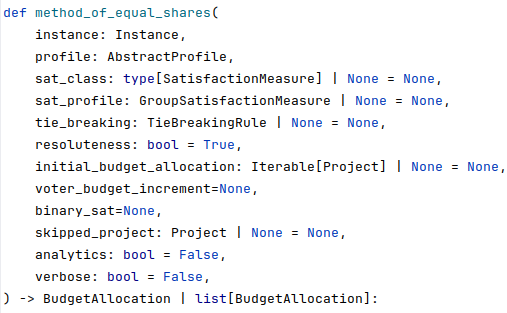
\includegraphics[width=0.7\textwidth]{figures/MES_method_pabutools.png}
  \caption{Function header for MES in Pabutools, showcasing most important data structures used throughout Pabutools.}
  \label{fig:myplot}
\end{figure}
It is important to note that election rules may choose different outcomes depending on the \emph{SatisfactionMeasure} they were called with. \emph{SatisfactionMeasure} is an abstract class representing a satisfaction measure for a given ballot. Two of the most important satisfaction measures for us are \emph{cost satisfaction measure} and \emph{additive cardinal satisfaction measure}.
\section{Integration of additive Stable-Priceability}
Implementation for finding and verifying priceable and stable priceable allocations already existed in the Pabutools library as part of analysis subpackage. However, it only supported profiles of \emph{AbstractApprovalProfile}. We extend it more broadly to \emph{AbstractProfile}, as it is the superclass of both \emph{ApprovalProfile} and \emph{CardinalProfile}. \emph{OrdinalProfile} is not supported though and it is explicitly rejected in the implementation. If the open-source community decides to provide a mapping from ordinal ballots to cardinal ballots, the ordinal setting could also be then served by this implementation.
\begin{figure}[H]         
  \centering              
  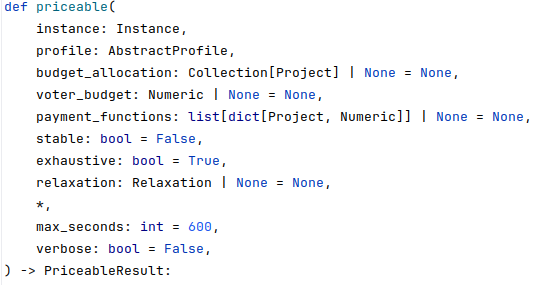
\includegraphics[width=0.7\textwidth]{figures/Priceable_function_header.png}
  \caption{Function header for stable priceability in Pabutools.}
  \label{fig:myplot}
\end{figure}
The above method either finds or verifies simple priceable allocations when \emph{stable := False} or stable-priceable allocations otherwise. Our work consisted only of updating the notion of stable-priceability, therefore implementation for simple priceability remained unchanged, except for updating the notion of supporting a candidate to cardinal ballots.

In order to reuse the same code for approval and cardinal ballots, minor changes to ballot classes were also added: functions \emph{utility} and \emph{supports}. For abstract ballot, the default implementation raises \emph{NotImplementedError}.
\begin{figure}[H]
  \centering
  \begin{minipage}{0.4\textwidth}
    \centering
    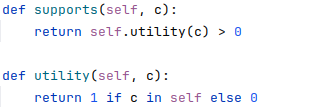
\includegraphics[width=\linewidth]{figures/cardinal_utility.png}
    \caption{Mentioned functions in CardinalBallot class.}
    \label{fig:img1}
  \end{minipage}\hfill
  \begin{minipage}{0.4\textwidth}
    \centering
    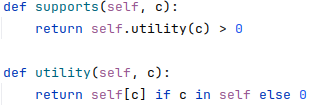
\includegraphics[width=\linewidth]{figures/approval_utility.png}
    \caption{Mentioned functions in ApprovalBallot class.}
    \label{fig:img2}
  \end{minipage}
\end{figure}

Additionally, stability relaxations have been adjusted to account for new definition of stable priceability. Though now they work with any additive utilities, their behaviour has only been studied and tested in the case of binary utilities. Extending and empirically studying these relaxations for cardinal ballots remains future work; Pabutools is structured to support this exploration with minimal changes.
\section{Testing}
To ensure the correctness of the implementation and the theoretical soundness of the proposed extension, a set of tests was also added to the project. The Pabutools library already contained some test cases for approval-based implementation of the \emph{priceable} function. They consisted of a couple of small, very well-understood instances for which solutions are known from manual analysis and prior literature, often coming from examples from papers on the subject and from the website on the Method of Equal Shares~\cite{EqualSharesWebsite}.

A key part of the tests aim to verify, that the updated function does indeed reduce to previous, approval-only implementation, in order not to break existing analysis tools and provide backwards compatibility. Pre-existing tests are reused for this, as the solution is expected to be exactly the same. A test was also added to verify if the new implementation does imply core up-to-one.

Finally, a new set of tests based on deeply analysed cardinal-based instances are added, to verify implementation for slightly more complex scenarios. These instances, similar in spirit to original set of tests, provide strong arguments for the correctness of the new implementation.

\chapter{Empirical Evaluation}\label{chap:4}
\section{Available data description}
Pabutools library contains hundreds of historical, real-life instances of participatory budgeting elections, from numerous Polish cities such as Warsaw, Częstochowa, Poznań, Gdańsk and more. Elections contain both city-wide vote profiles, as well as profiles specific for cities' districts. Elections vary greatly in size, with the number of voters ranging from less than $100$ to over $100,000$ with over $200$ projects available.

Most of the available instances are approval-based elections. However, we treat them as if cardinal ballots were cast, where the utility from a supported project is equal to its cost, that is we use cost satisfaction measure. A minority of instances allow for \emph{cumulative ballots}, which are cardinal profiles with additional constraints. Voters are allowed to split some number of points among projects, with minimal and maximal number of points being assignable to a single candidate. Also a small group of instances are ordinal-based elections, where voters sort the projects by their preference. Because stable priceability is not defined for this type of ballots, we do not evaluate our work on these instances.

In total, we analyse $96$ instances of elections with cumulative profiles and $398$ elections with approval profiles. The instances were selected from the Pabulib library in ascending order of the product $(\text{number of voters})\cdot(\text{number of projects})$, as this is the factor defining the size of the linear program. Some of the larger instances in the repository have been omitted due to computational constraints. As problem size increases, solver runtime grows rapidly. We therefore imposed a fixed wall-clock limit and excluded instances exceeding it.  In the next sections, we test different voting rules and check their effectiveness in finding priceable and stable-priceable outcomes, as well as look at how often exhaustive outcomes prove to be stable-priceable.

All scripts used to process the election data, run the experiments and generate the results presented in this chapter are available in a public repository~\cite{Chapter4Scripts}.
\section{Existence of stable-priceable allocations}
We consider the following election rules:
\begin{itemize}
    \item MES --- the classic Method of Equal Shares
    \item MES+BOS --- MES with Bounded Overspending
    \item MES+Inc --- MES with voter budget increment
    \item MES+Inc+UGreedy --- MES with voter budget increment and greedy fill
    \item UGreedy --- the classic utilitarian greedy method.
\end{itemize}
Firstly, we consider elections with cumulative profiles, with \emph{AdditiveCardinalSat} satisfaction measure. That is, a voter $i$'s satisfaction of the outcome $W$ is equal to the sum of scores assigned to $W\cap A(i)$.
\begin{figure}[H]         
  \centering              
  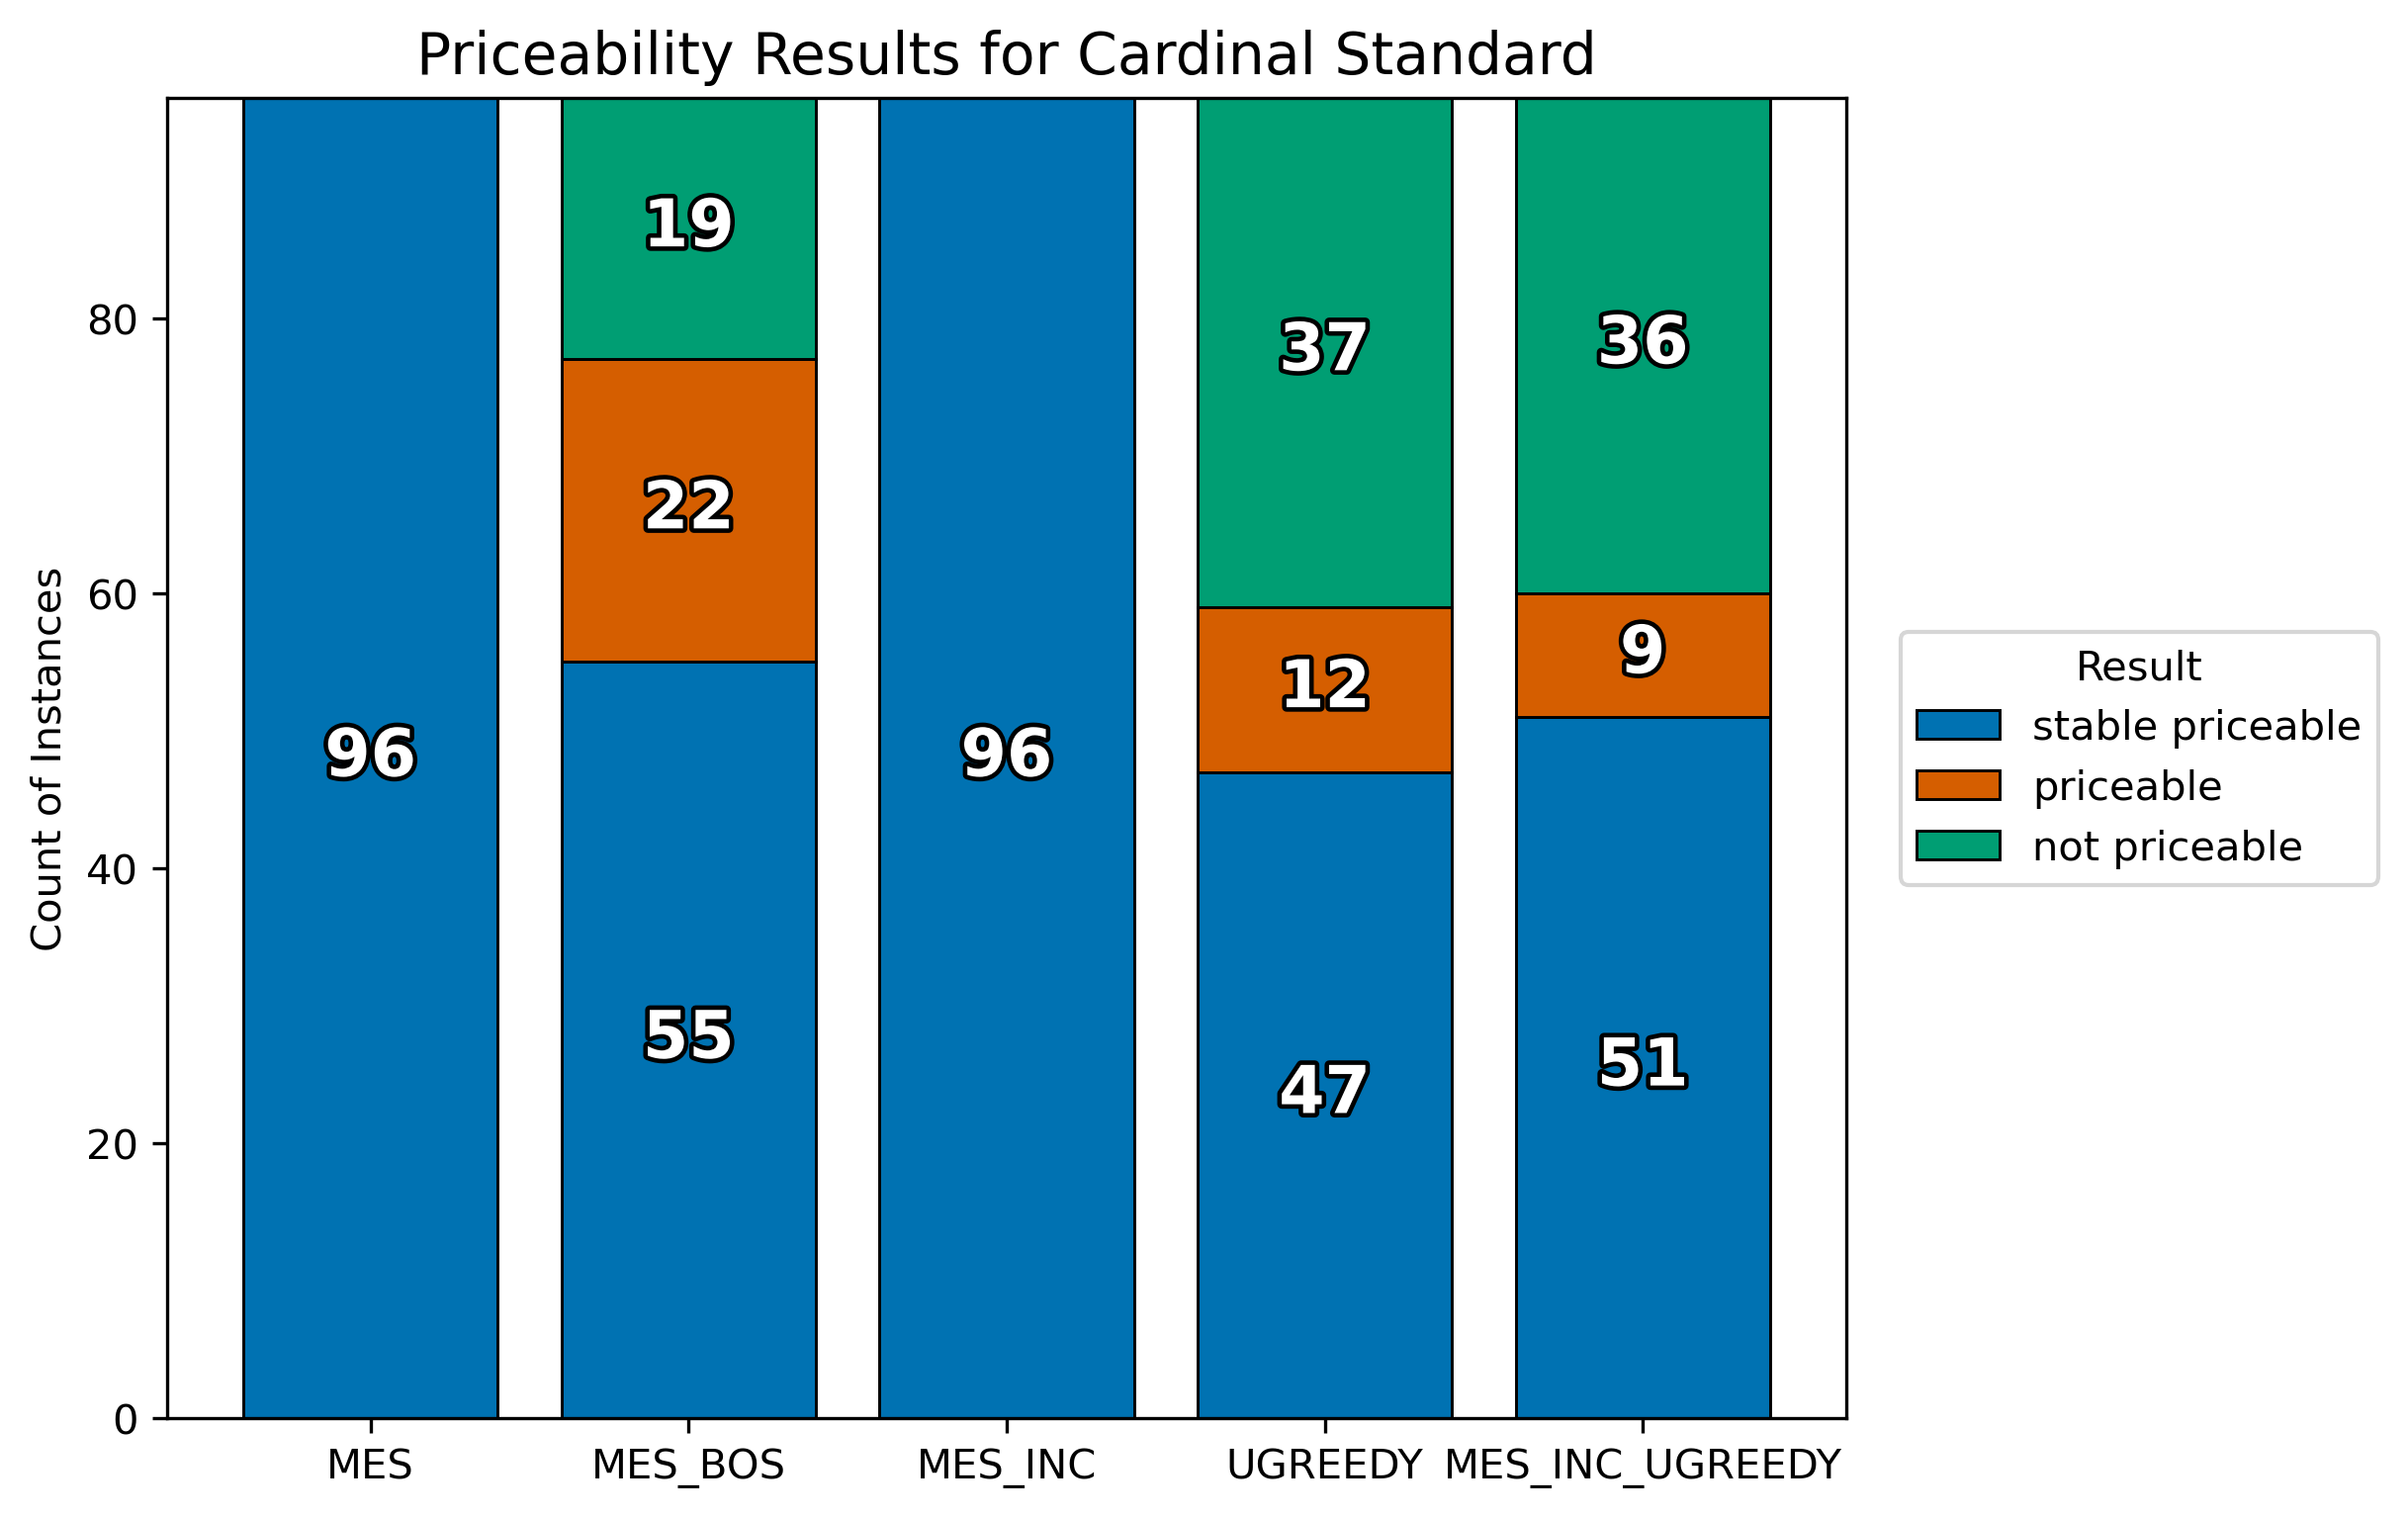
\includegraphics[width=0.7\textwidth]{figures/plots/cardinal-standard/cardinal_standard_priceability.png}
  \caption{Stable priceability and priceability of allocations returned by selected election rules for unmodified cardinal-based elections.}
  \label{fig:myplot}
\end{figure}
When considering untouched cardinal-based elections, we can observe that pure MES and Mes+Inc score perfect $100\%$ of the allocations being stable priceable. The utilitarian greedy method provides stable priceable allocations only in less than half of all instances, while the MES filled with utilitarian greedy scores in between, but closer to pure UGreedy. This is expected, as the MES is proved to select very fair outcomes when working with the additive score satisfaction measure. MES with Bounded Overspending provides similar results to MES with greedy fill.


We also consider both elections with approval profiles and cumulative profiles. However, we adjust them to \emph{cost satisfaction measure}. Satisfaction score for each voter $i$ from a project $p$ is equal to the utility assigned by voter $i$ to $p$ multiplied by its cost $score_i(p)=u_i(p)\cdot cost(p)$. This is believed to be more representative of actual voters' satisfaction, as larger project typically bring greater satisfaction to their supporters. Naturally, our updated notion of stable priceability allows such an evaluation. Previously, analysis only for approval-based instances was possible.
\begin{figure}[H]         
  \centering              
  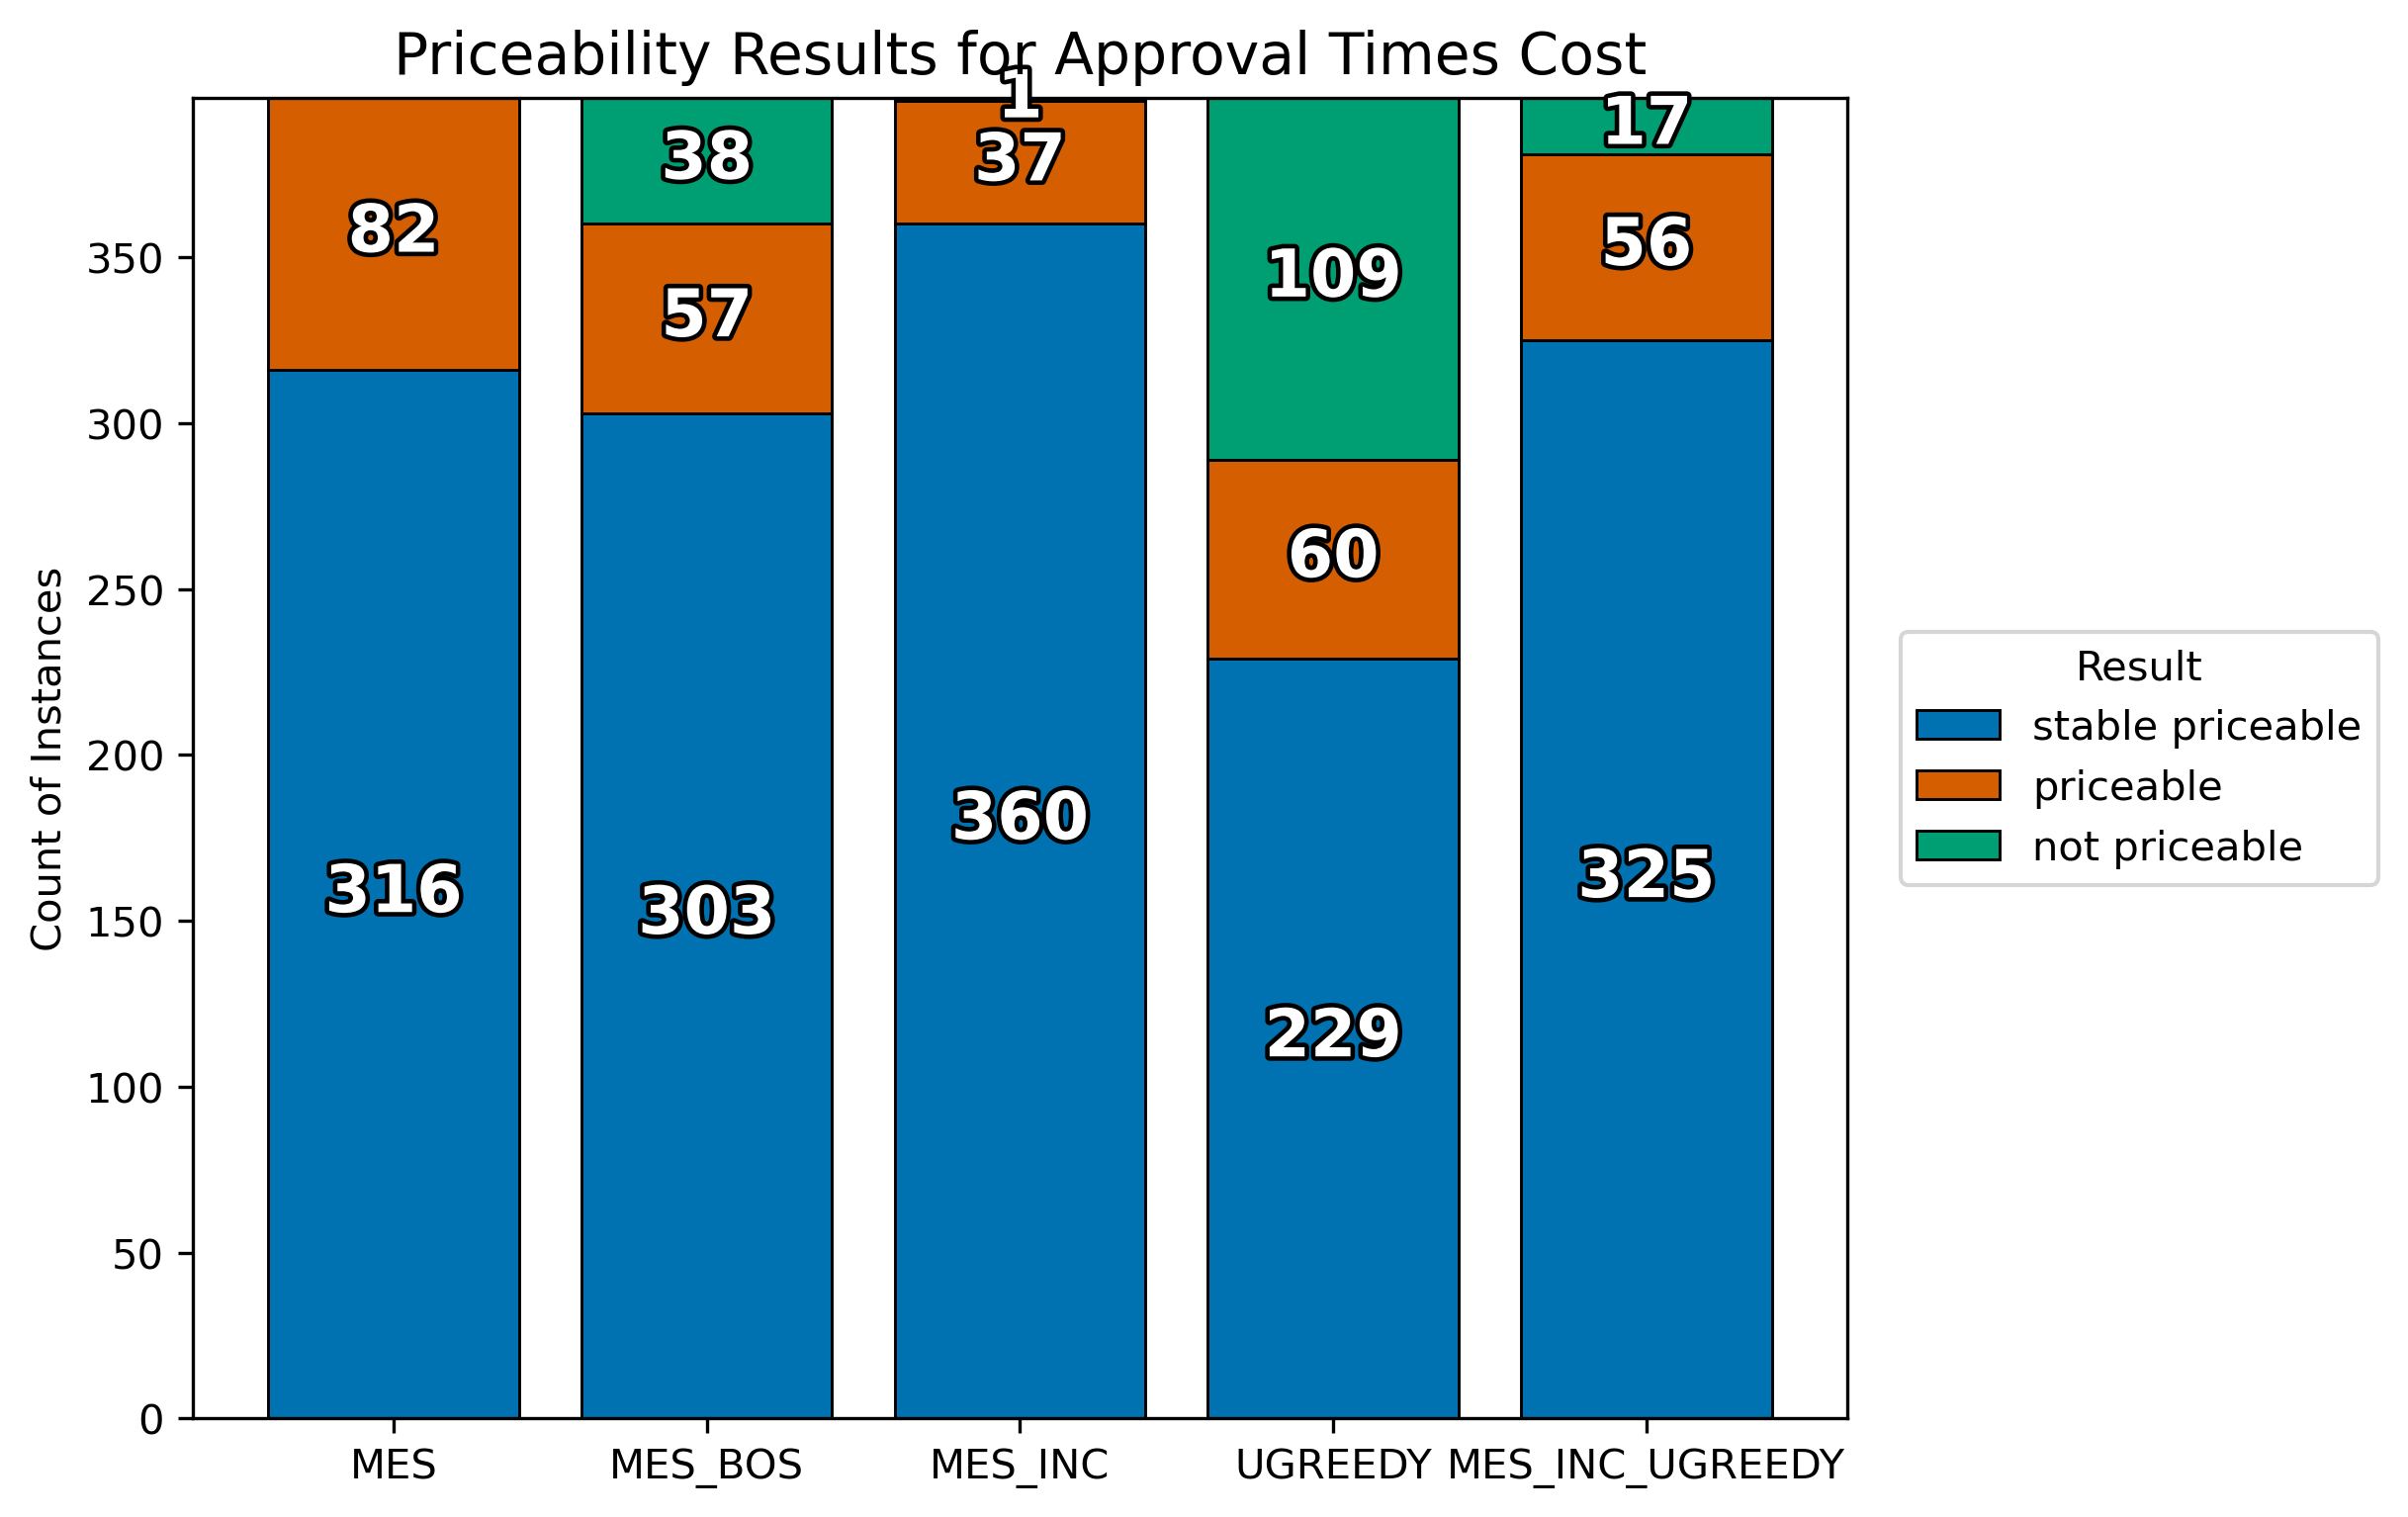
\includegraphics[width=0.7\textwidth]{figures/plots/approval-times-cost/approval_times_cost_priceability.png}
  \caption{Stable priceability and priceability of allocations returned by selected election rules for approval ballot instances multiplied by projects' costs.}
  \label{fig:myplot}
\end{figure}
As we can see from the plot above, the Utilitarian Greedy method performs by far the worst compared to variations of the Method of Equal Shares. Its primary aim of maximizing total voter utility often does not lead to returning proportional allocations. MES scores decently with around $79\%$ being stable priceable and the remainder priceable. Variation with voter budget increment does even better, with $90\%$ of stable priceable allocations. Again, filling MES allocations greedily until exhaustiveness affects priceability in a very negative way. BOS stands out the most for these instances, suggesting that it is more well-suited for cost satisfaction measure.
\begin{figure}[H]         
  \centering              
  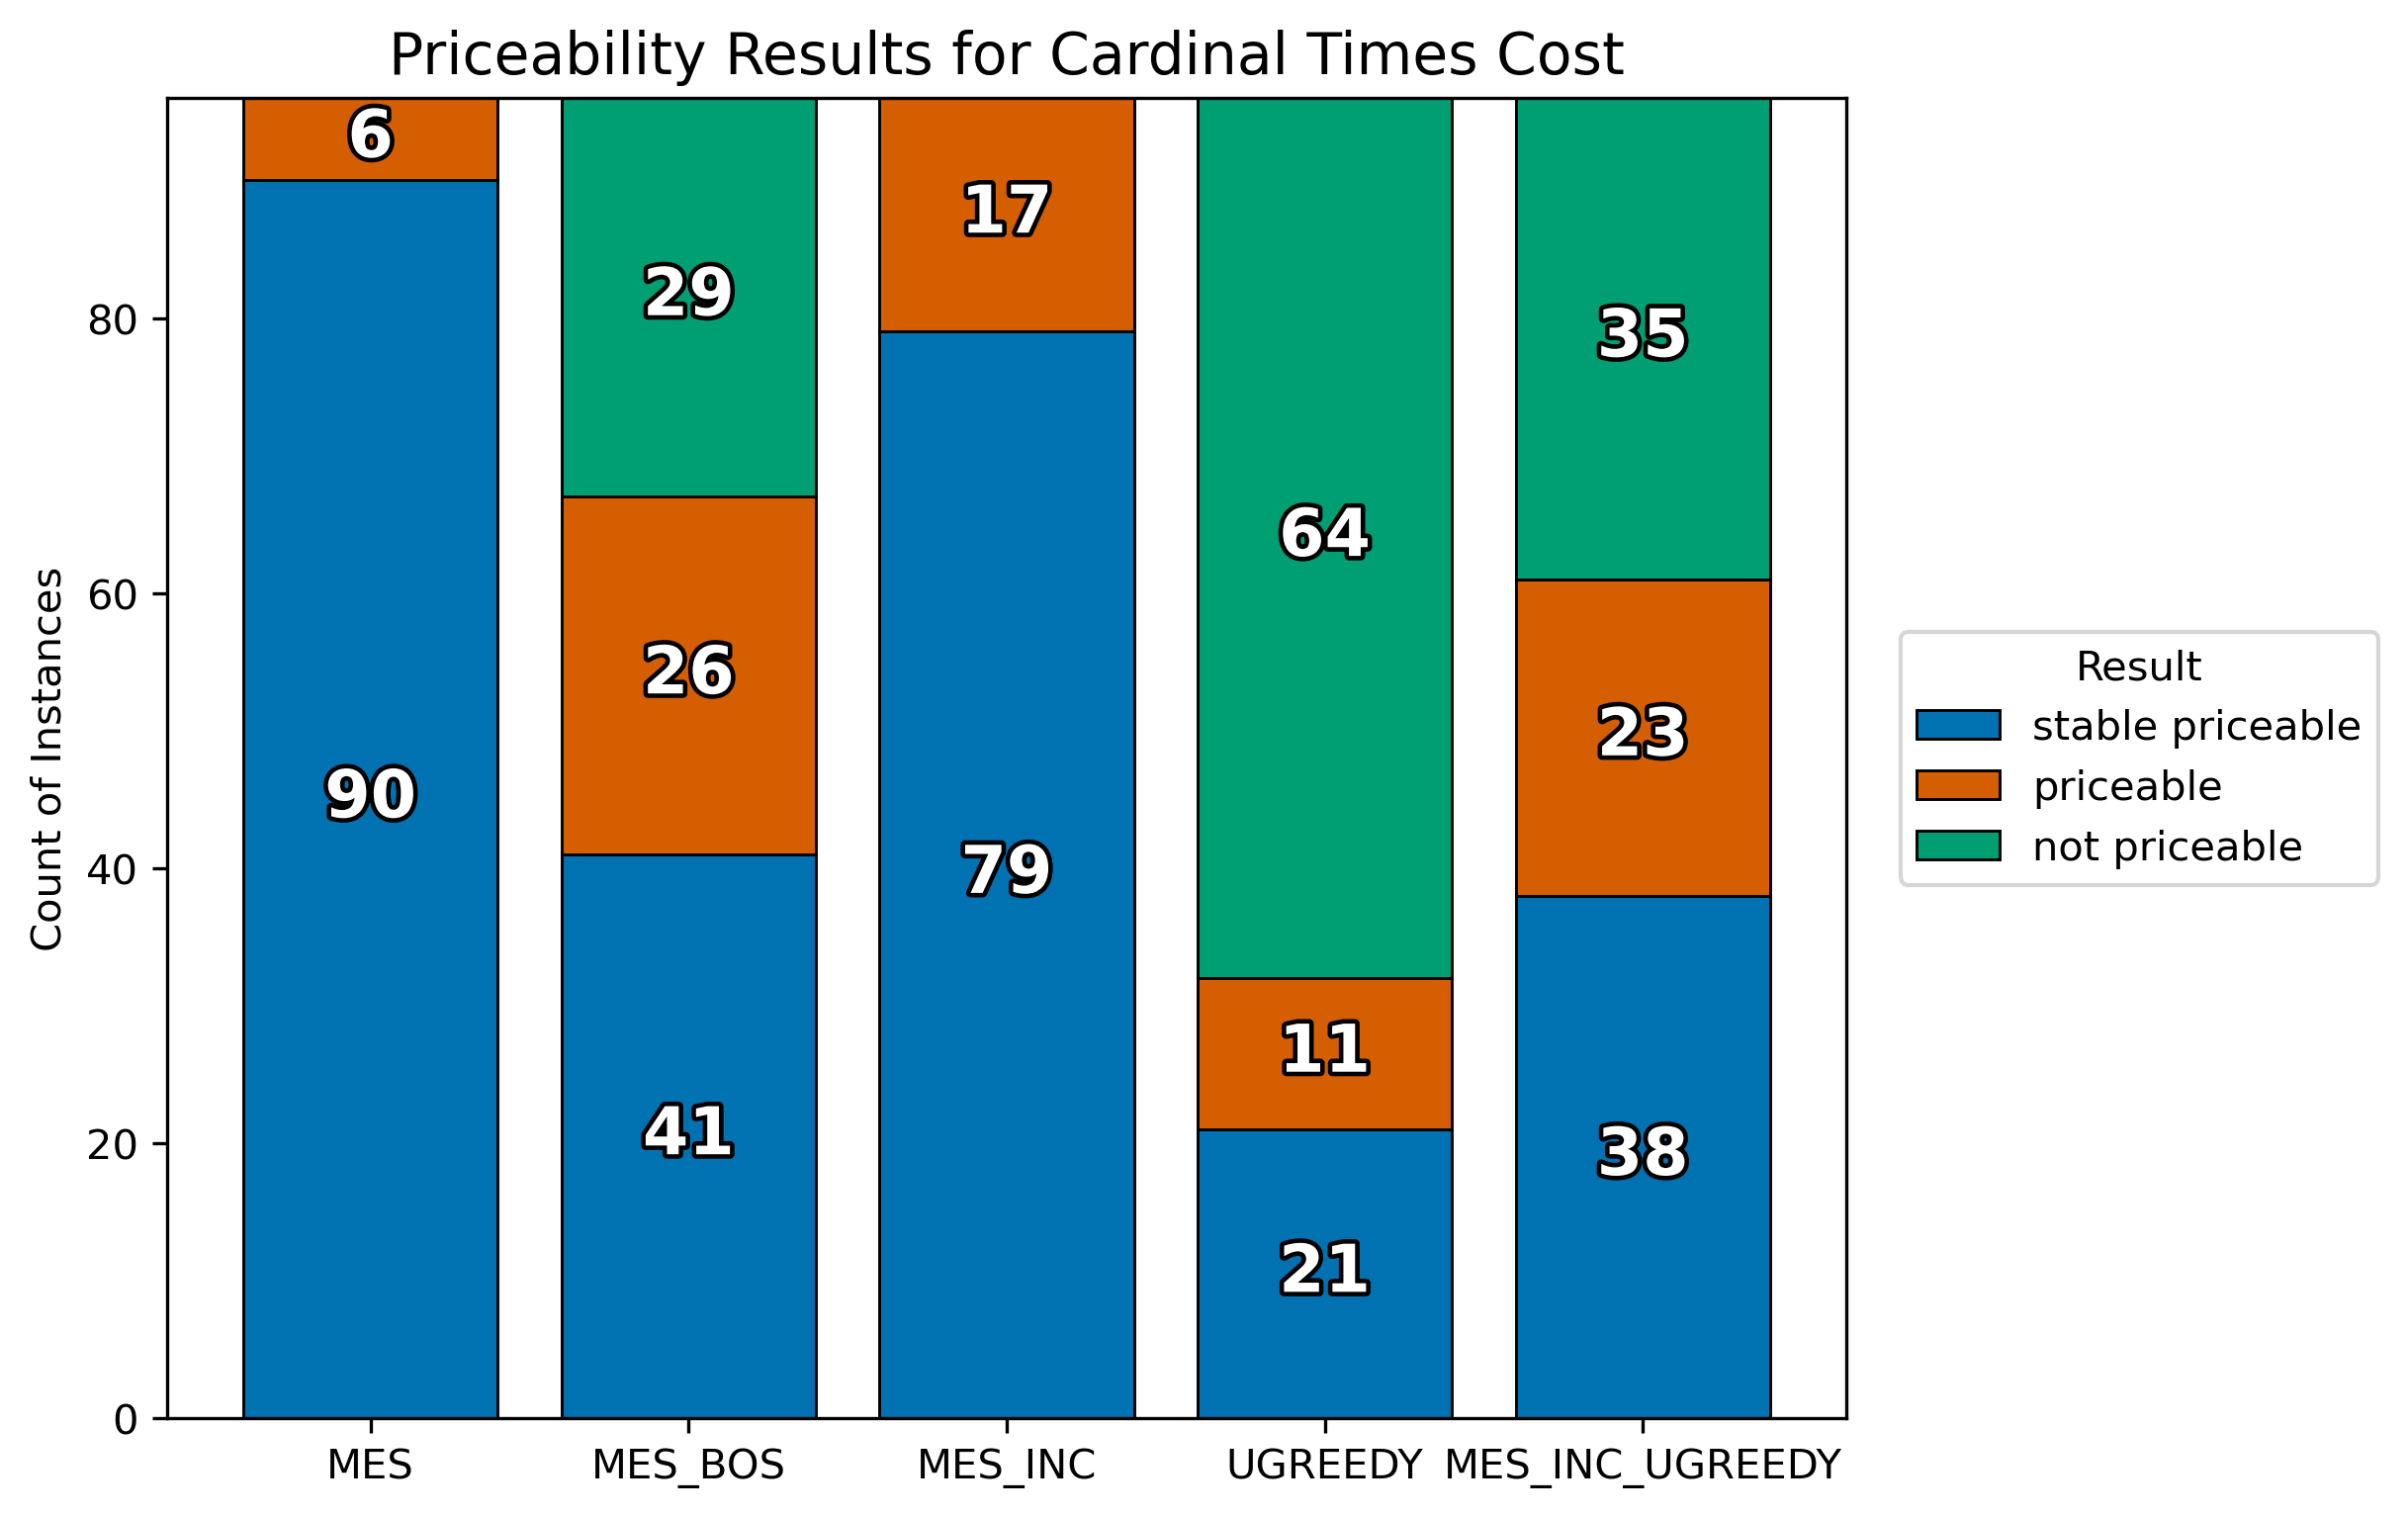
\includegraphics[width=0.7\textwidth]{figures/plots/cardinal-times-cost/cardinal_times_cost_priceability.png}
  \caption{Stable priceability and priceability of allocations returned by selected election rules for cardinal ballot instances multiplied by projects' costs.}
  \label{fig:myplot}
\end{figure}
For cardinal ballots, after multiplying each utility by project cost, we see that pure MES performs best, with MES with increment budget dropping a few stable priceable results from original rule. This can be considered surprising, because it differs from the results from approval-based instances. Potentially, it is a matter for further research. Utilitarian greedy returns stable priceable in just over $\sfrac{1}{4}$ of instances, a rather underwhelming score compared to other evaluated election rules. MES with Bounded Overspending performs again more similar to MES with greedy fill, significantly worse compared than with approval-based elections and cost utilities.

We also summarise the results from all election rules and check, if any of them was able to find a stable priceable, or at least a priceable allocation.
\begin{figure}[H]         
  \centering              
  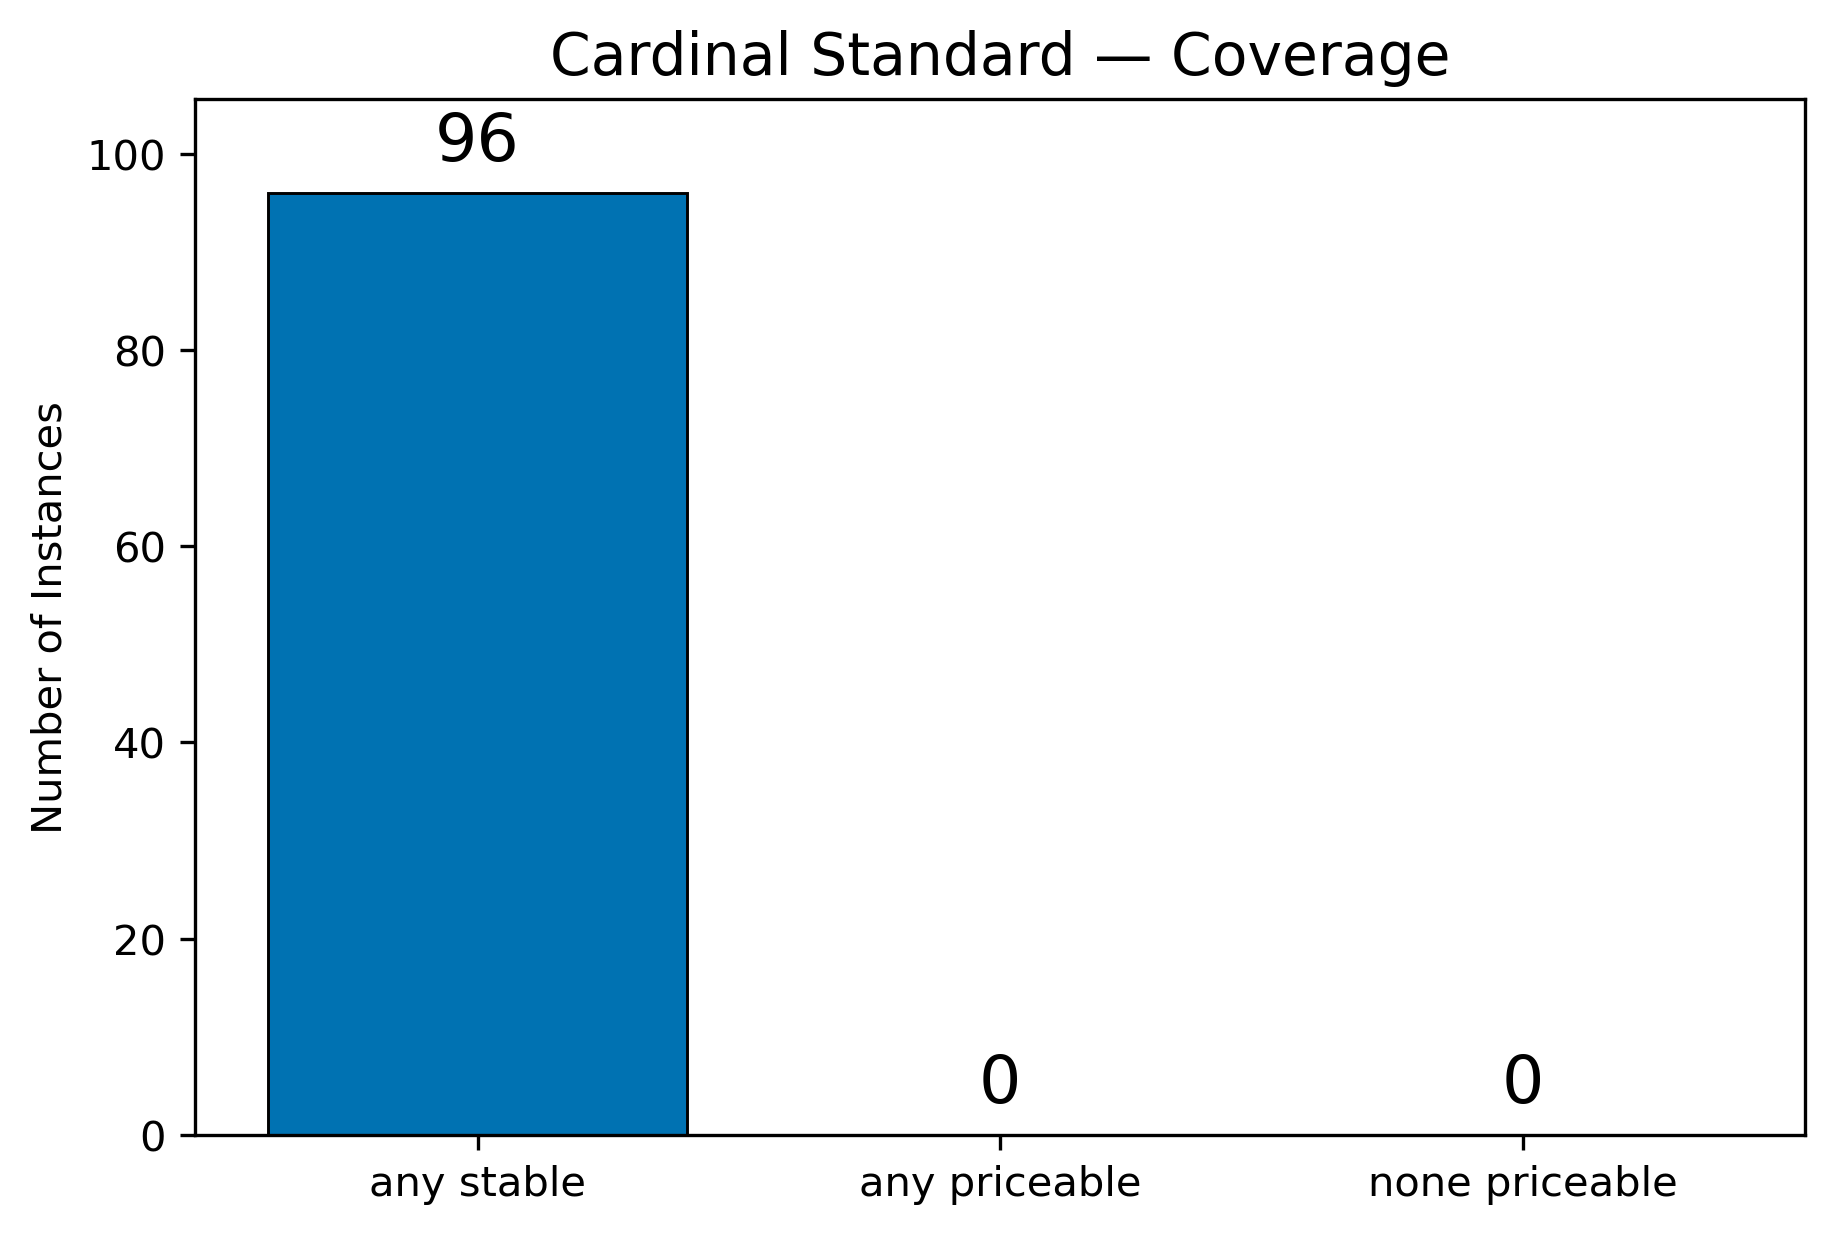
\includegraphics[width=0.7\textwidth]{figures/plots/cardinal-standard/cardinal_standard_coverage_non_exhaustive.png}
  \caption{Number of instances of elections for standard cardinal-based elections, for which any rule was able to return a stable priceable, or a priceable allocation.}
  \label{fig:myplot}
\end{figure}
\begin{figure}[H]         
  \centering              
  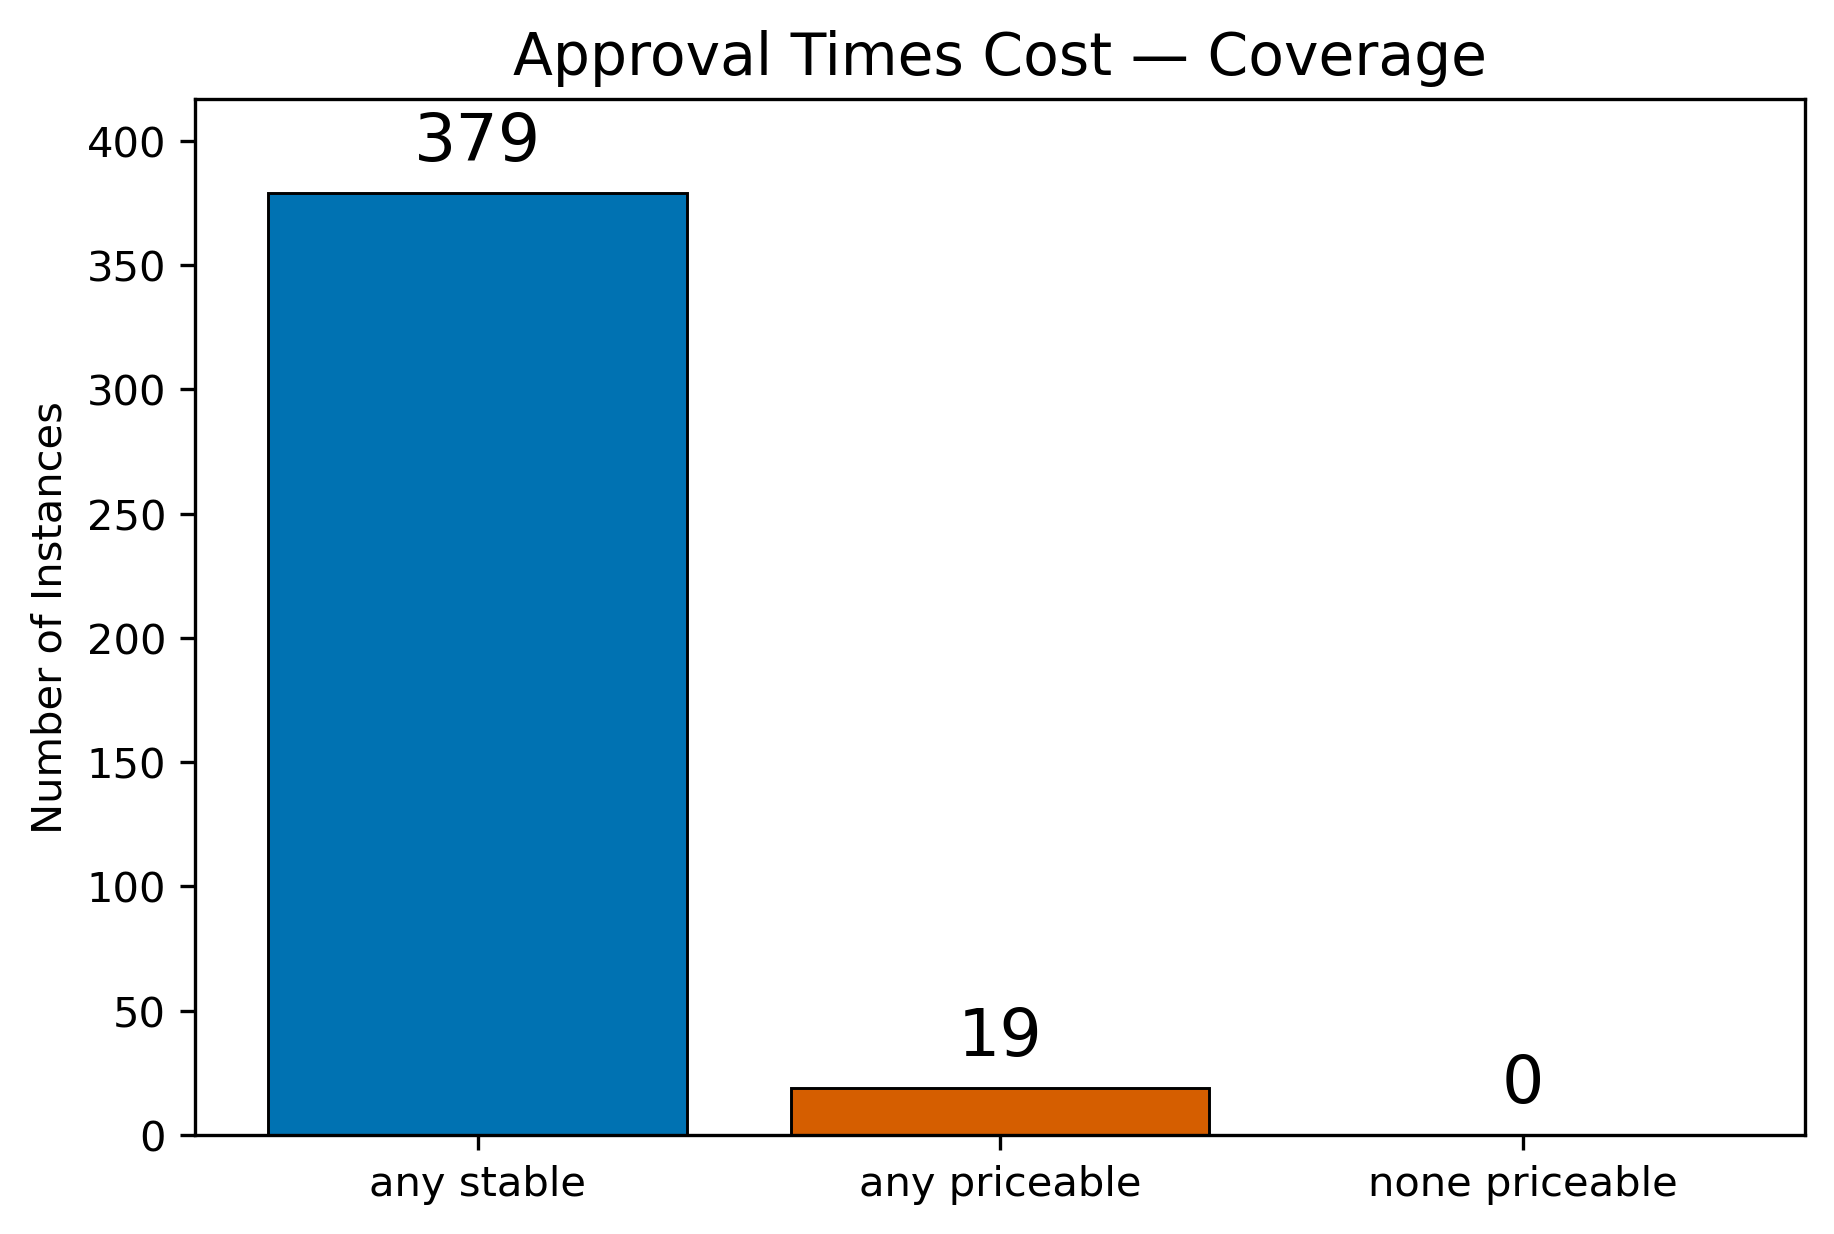
\includegraphics[width=0.7\textwidth]{figures/plots/approval-times-cost/approval_times_cost_coverage_non_exhaustive.png}
  \caption{Number of instances of elections for standard approval-based ballot instances multiplied by projects' costs, for which any rule was able to return a stable priceable, or a priceable allocation.}
  \label{fig:myplot}
\end{figure}
\begin{figure}[H]         
  \centering              
  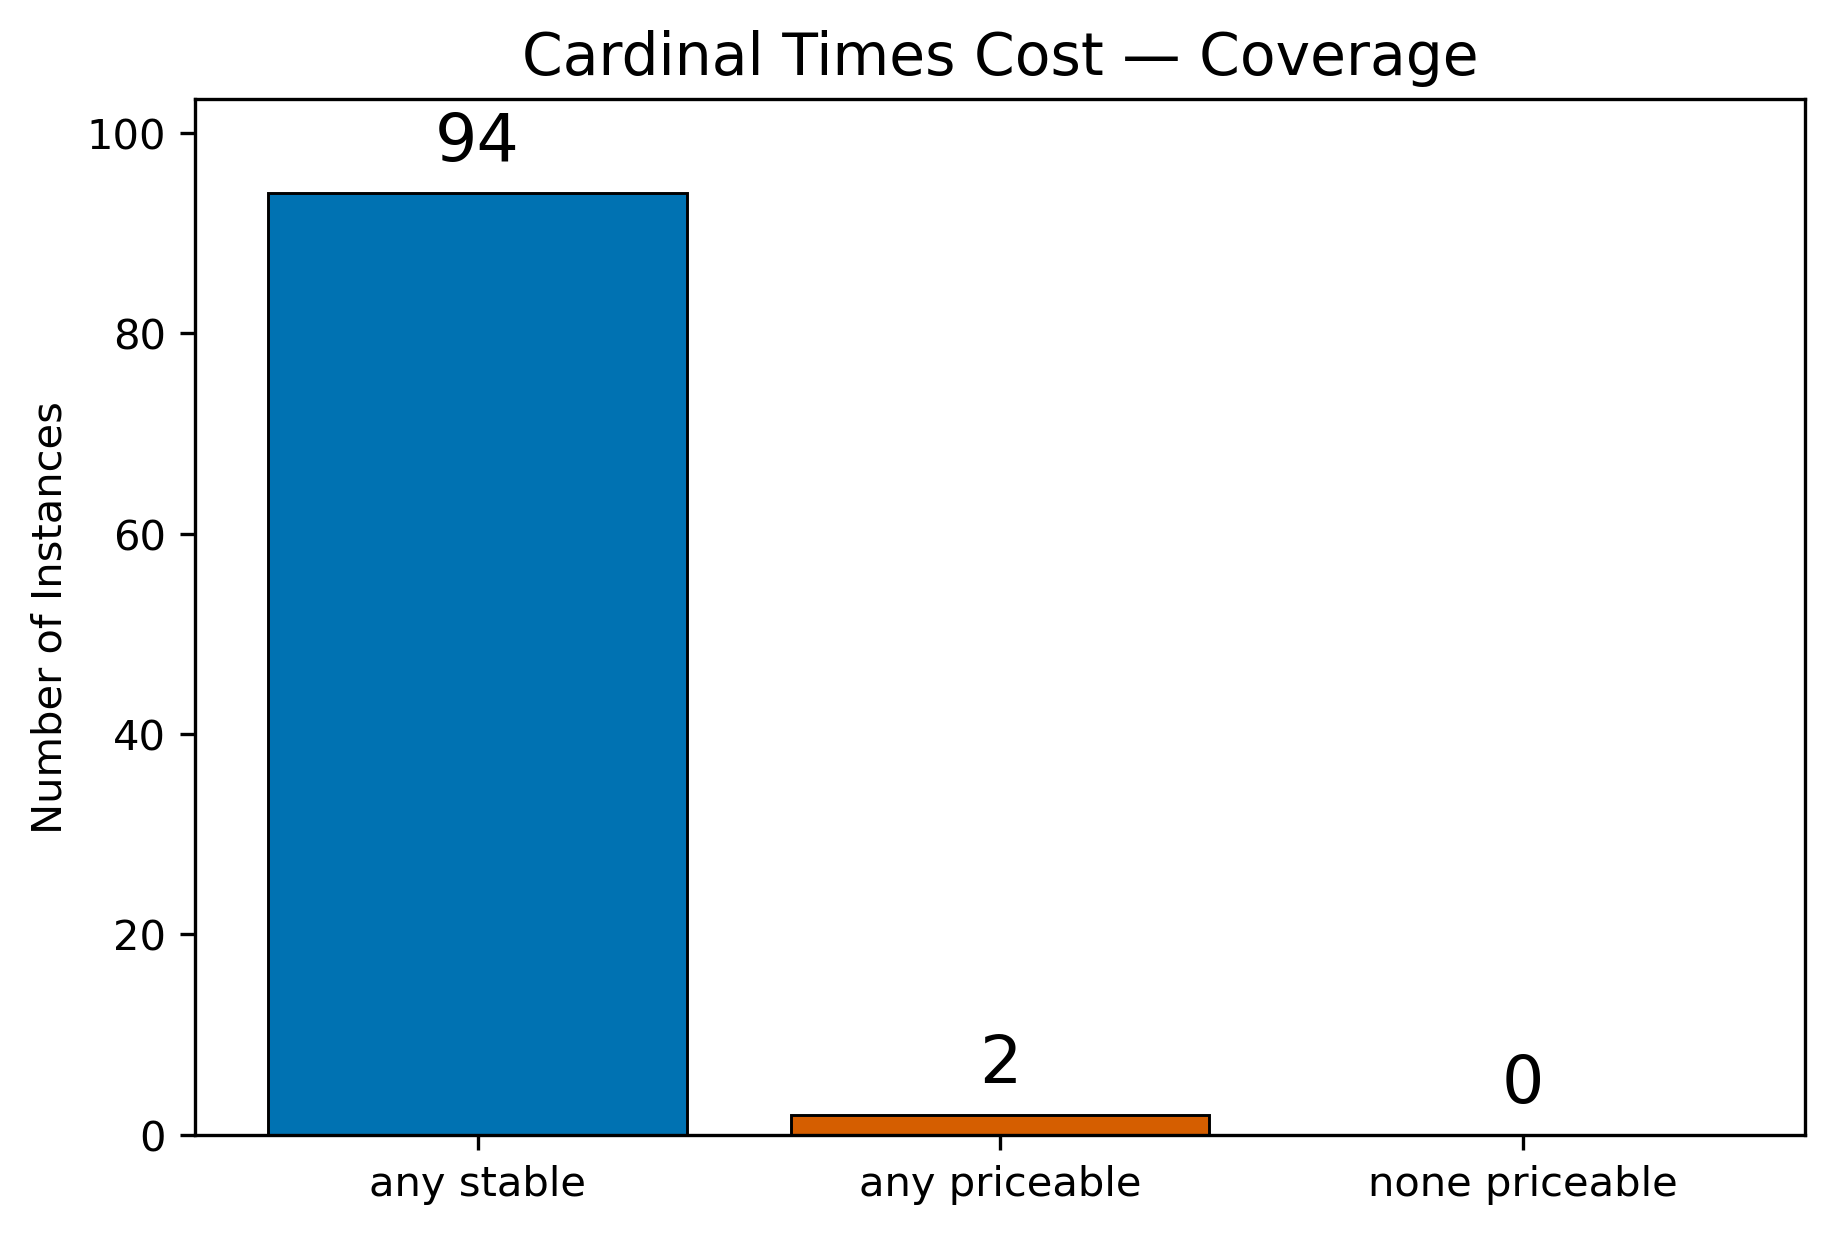
\includegraphics[width=0.7\textwidth]{figures/plots/cardinal-times-cost/cardinal_times_cost_coverage_non_exhaustive.png}
  \caption{Number of instances of elections for standard cardinal-based ballot instances multiplied by projects' costs, for which any rule was able to return a stable priceable, or a priceable allocation.}
  \label{fig:myplot}
\end{figure}
A priceable solution was always found. However --- when using cost satisfaction measure, we observe that a stable priceable solution was not always returned by any of the tested methods. This does not mean, that the methods behaved poorly, as such solutions might not always exist.
\begin{figure}[H]         
  \centering              
  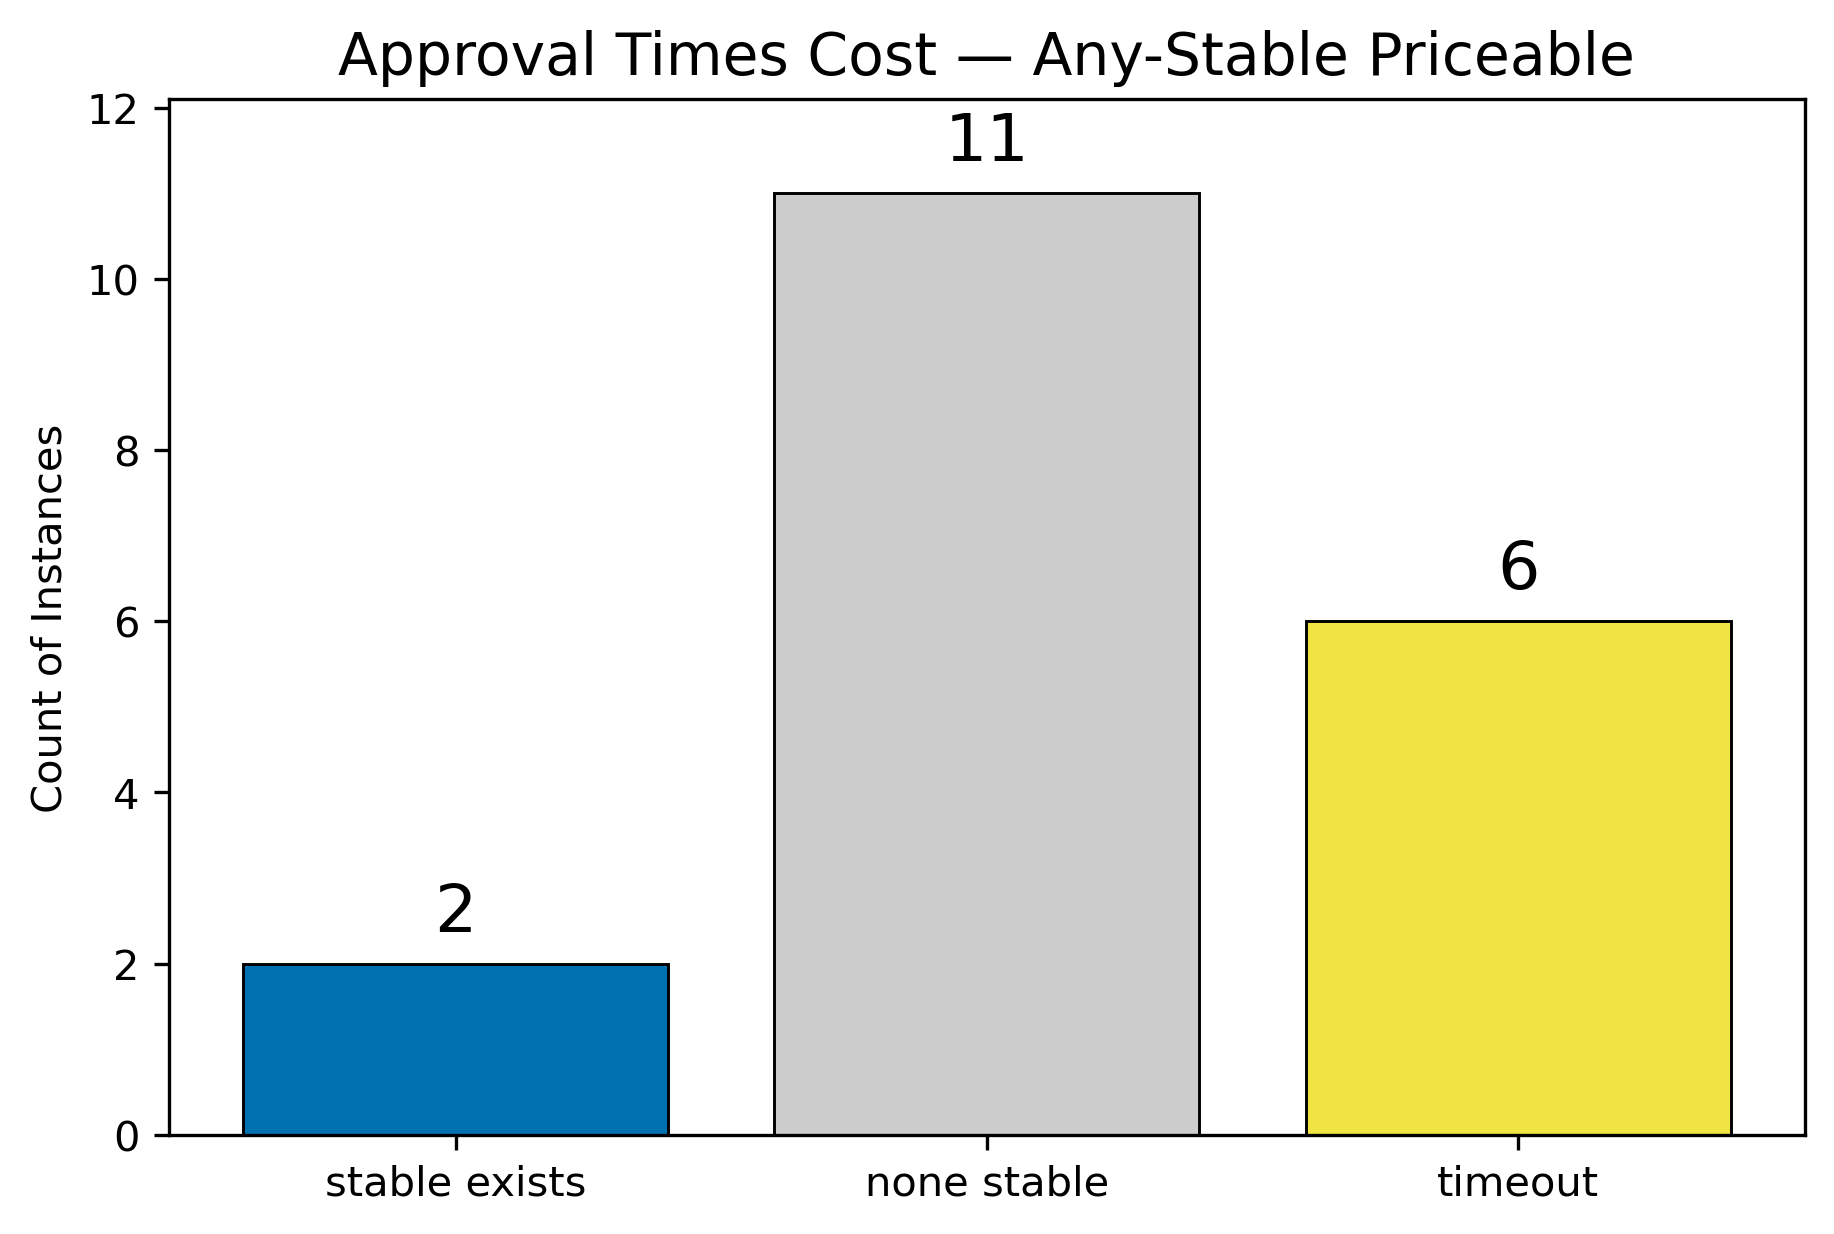
\includegraphics[width=0.7\textwidth]{figures/plots/approval-times-cost/approval_times_cost_any_stable_non-exhaustive.png}
  \caption{Number of instances of elections with approval ballots and cost satisfaction measure, for which no election rule returned a stable priceable allocation, where such a solution exists or does not.}
  \label{fig:myplot}
\end{figure}
\begin{figure}[H]         
  \centering              
  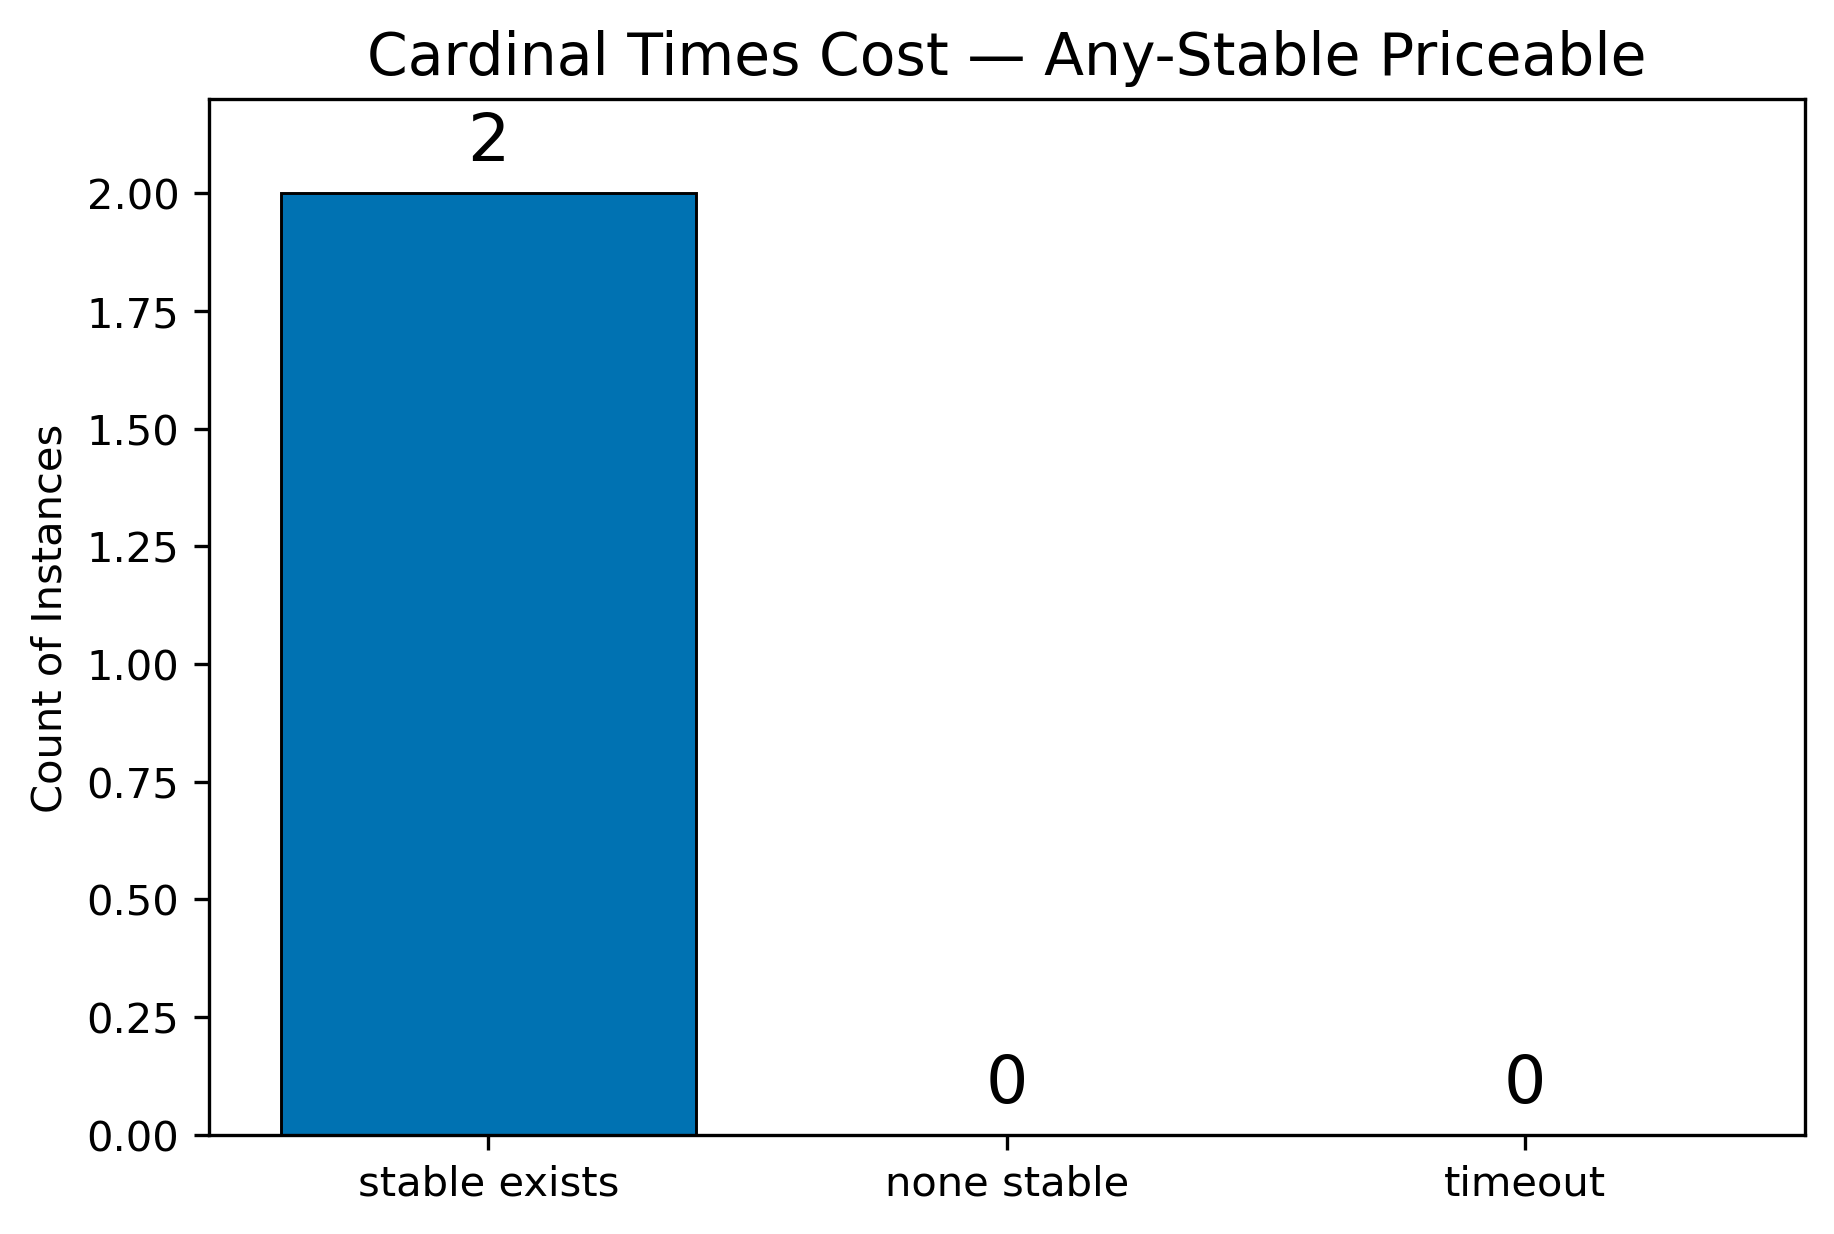
\includegraphics[width=0.7\textwidth]{figures/plots/cardinal-times-cost/cardinal_times_cost_any_stable_non-exhaustive.png}
  \caption{Number of instances of elections with cardinal ballots and cost satisfaction measure, for which no election rule returned a stable priceable allocation, where such a solution exists or does not.}
  \label{fig:myplot}
\end{figure}
In majority of cases, no stable priceable solution exists at all, meaning evaluated election rules did exceptionally well at finding existing stable priceable allocations. We also note a number of elections, when the \emph{priceable} function timed out within our time limit for the largest election instances. We accept this, as finding an allocation is a more difficult task than pure evaluation of a given result, and see this as area for further research with stronger computers and larger time limits.
\section{Exhaustive priceable and stable priceable outcomes}
As previously stated, it is highly beneficial for an election rule to return stable priceable, or at least, priceable outcomes. 

However, it is known that there exist election instances which do not have exhaustive priceable allocations. We say that an allocation is exhaustive if no unchosen project can be added to the allocation, without going over the total budget.
\begin{example}
Consider the following simple election with total budget $b:=3$, where choosing the only exhaustive allocation involves selecting a candidate with no supporters.
\begin{table}[H]
\centering
\begin{tabular}{lllccc}
\toprule
        & cost & $\#app$ & $v_1$ & $v_2$ & $v_3$\\
\midrule
\rowcolor{orange!10}
$c_1$& 1 & 0 & & &   \\
\rowcolor{orange!10}
$c_2$& 1 & 1 &  \app &  &        \\
\rowcolor{orange!10}
$c_3$& 1 & 2 &   & \app  & \app           \\
\bottomrule
\end{tabular}
\end{table}
It is clear that only choosing all candidates is exhaustive. However, that would mean that candidate $c_1$ also collects the total payment of $cost(c_1)=1$, which is against the notion that voters are only allowed to contribute funds towards candidates that they approve of.
\end{example}
It is usually sensible, to try to obtain exhaustive results. Intuitively, in a participatory budgeting setting, no voters would be against adding another project to the outcome, since they could either benefit from it or simply be indifferent to it in terms of their satisfaction. There are no obvious advantages to choosing non-exhaustive election rules in a a PB setting. 

While the Utilitarian greedy method is exhaustive by default, the Method of Equal Shares is not. This property of MES is meant to be fixed by its $2$ variations, including voter budget increment and greedy fill. BOS is also not exhaustive.

In this section, we look at the results obtained from all previously mentioned election rules and check, in how many instances they returned an exhaustive priceable or stable priceable outcome and which rule performed best.
\begin{figure}[H]         
  \centering              
  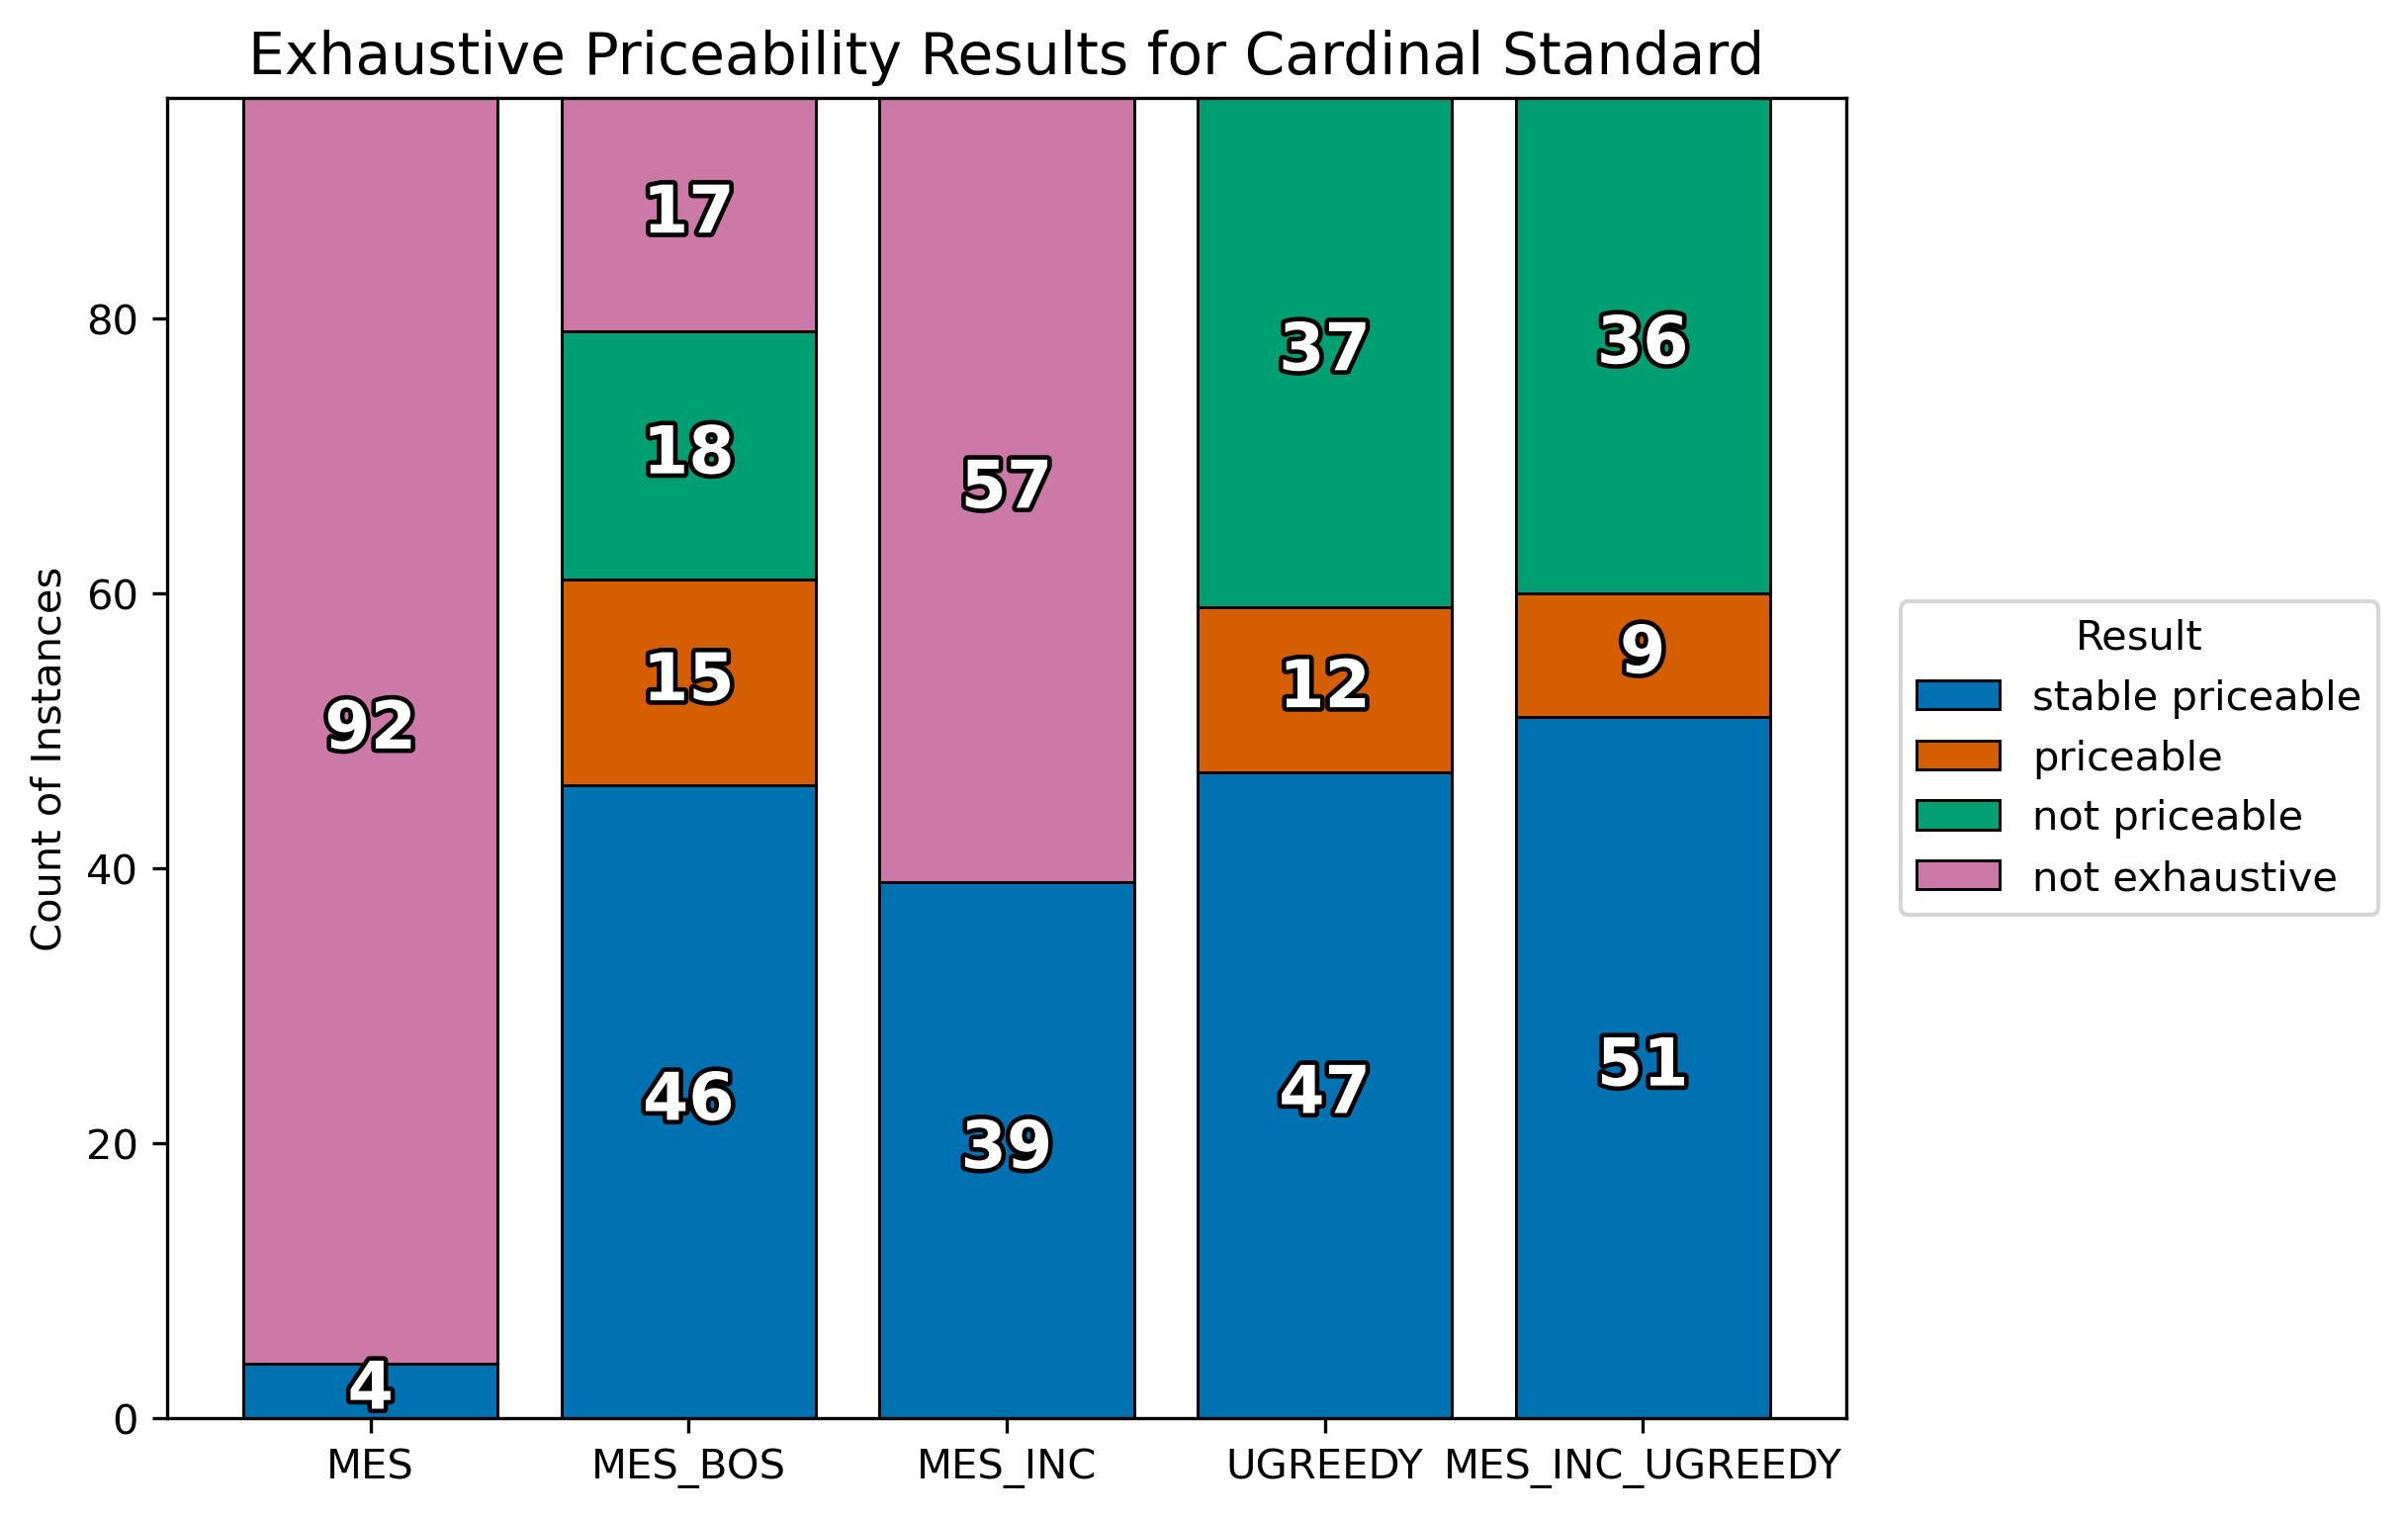
\includegraphics[width=0.7\textwidth]{figures/plots/cardinal-standard/cardinal_standard_exh_priceability.png}
  \caption{Exhaustive stable priceable and priceable allocations returned by selected election rules for unmodified cardinal-based elections.}
  \label{fig:myplot}
\end{figure}
\begin{figure}[H]         
  \centering              
  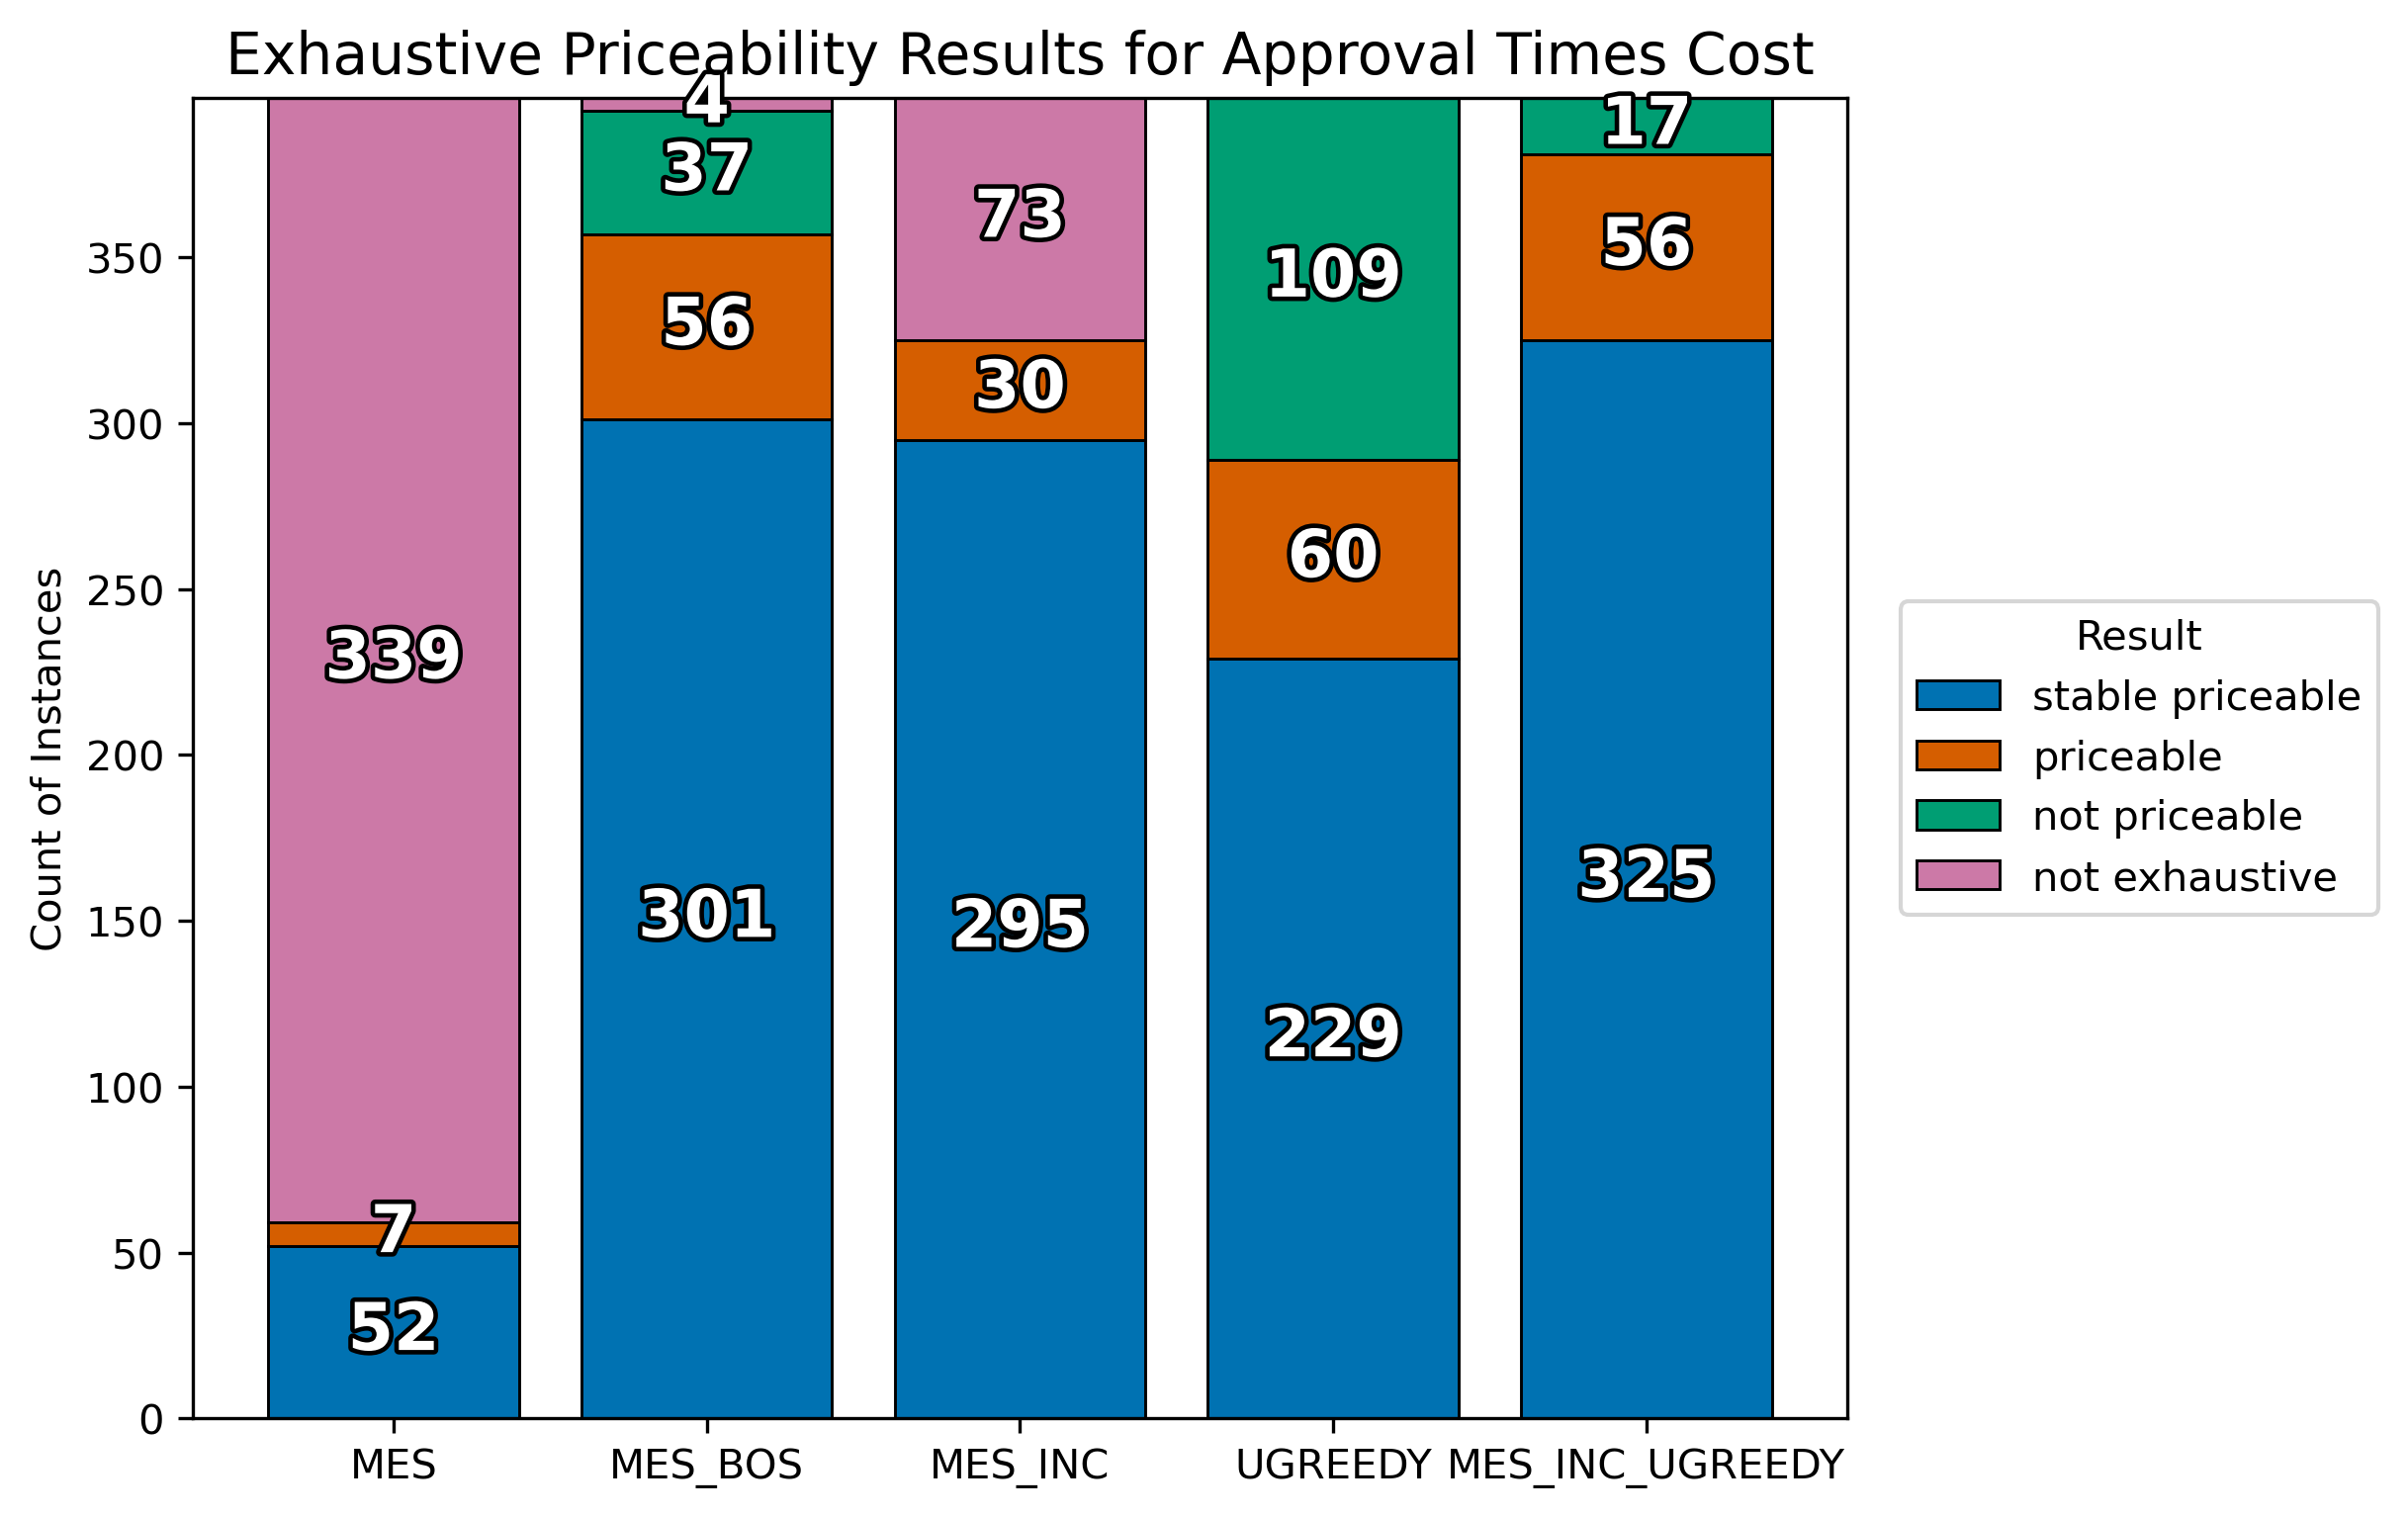
\includegraphics[width=0.7\textwidth]{figures/plots/approval-times-cost/approval_times_cost_exh_priceability.png}
  \caption{Exhaustive stable priceable and priceable allocations returned by selected election rules for approval-based elections with utilities multiplied by projects' costs.}
  \label{fig:myplot}
\end{figure}
\begin{figure}[H]         
  \centering              
  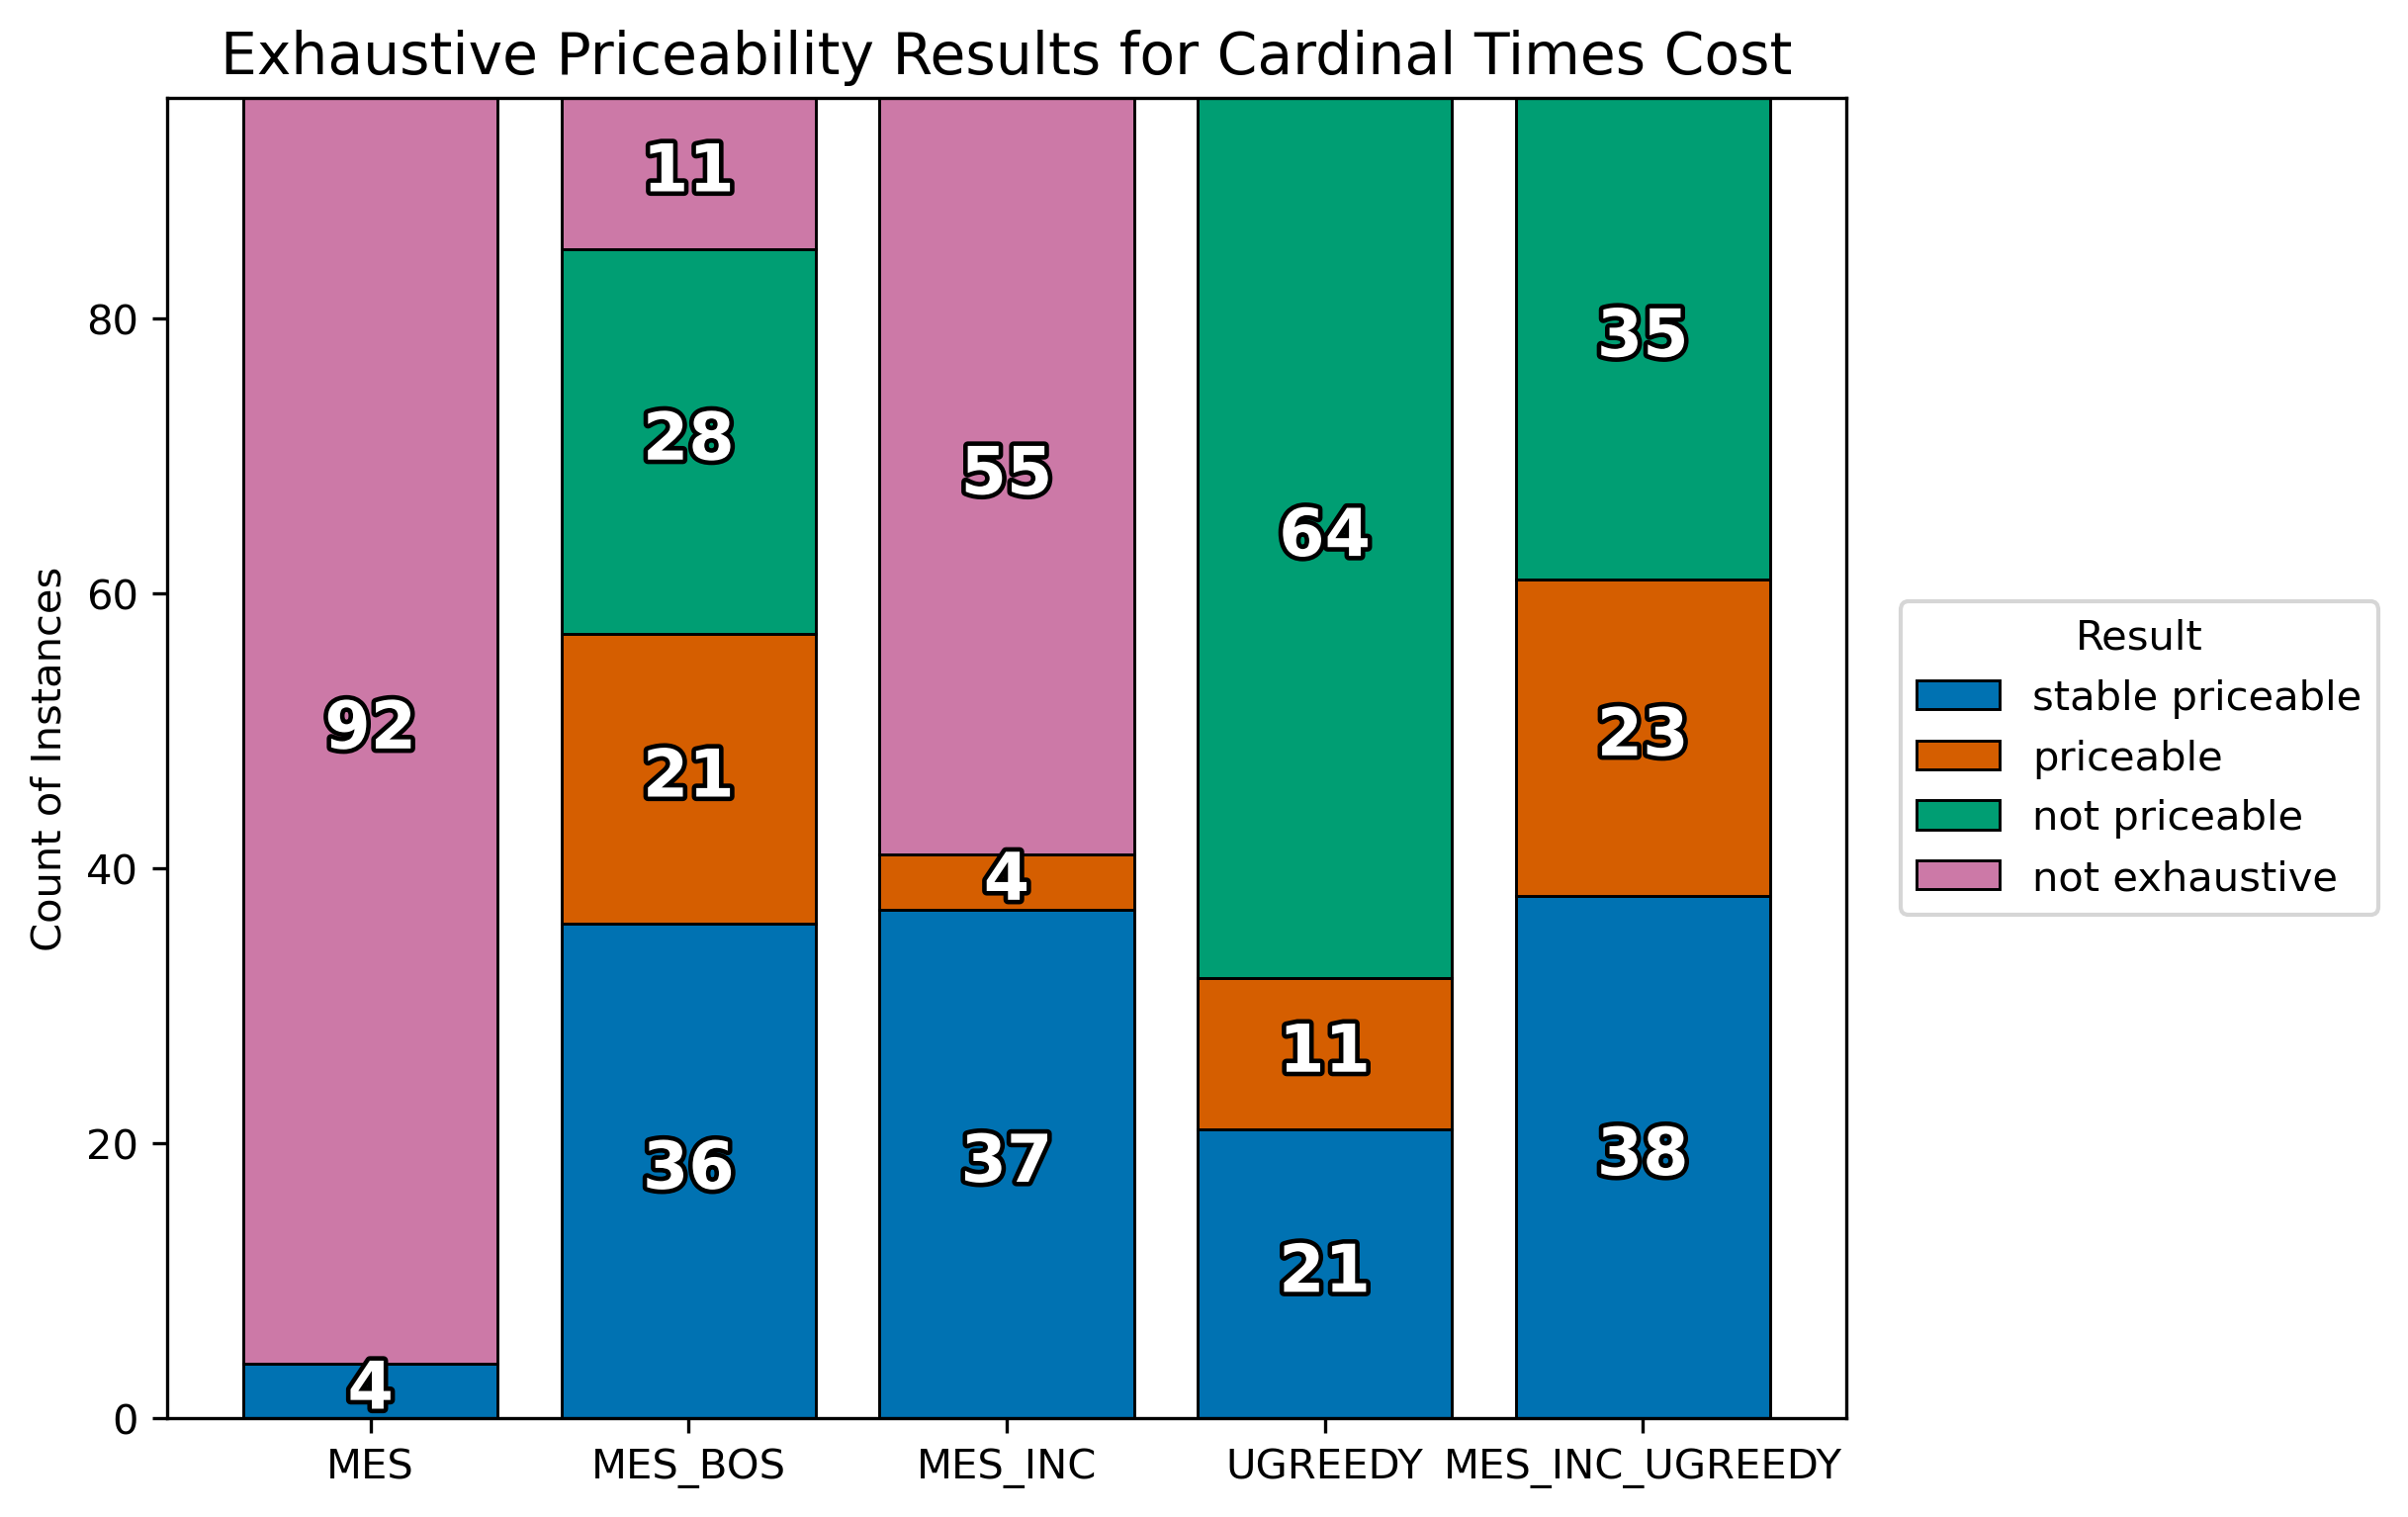
\includegraphics[width=0.7\textwidth]{figures/plots/cardinal-times-cost/cardinal_times_cost_exh_priceability.png}
  \caption{Exhaustive stable priceable and priceable allocations returned by selected election rules for approval-based elections with utilities multiplied by projects' costs.}
  \label{fig:myplot}
\end{figure}
As classic MES rarely returns exhaustive allocations at all, it almost never returns stable priceable exhaustive allocations, and it can be considered useless in this setting. However, when running the version with voter budget increment, its efficiency jumps to almost $74\%$ for approval elections with cost utilities and over $38\%$ for cardinal elections with cost utilities. Though BOS is not a variation meant to simply fix exhaustiveness, we observe significant improvements over classic MES. Utilitarian greedy scores just as well as with original constraints, and the same applies for MES with UGreedy fill. What stands out is that for elections originally in the cardinal setting, all methods do significantly worse compared to approval-based, though it was not visible without the exhaustive clause. It is either a sign of cost utilities being less proportional on their own, or that evaluated methods' approach does not efficiently grasp the concept of this kind of proportionality measurement.

So far, we have compared each rule’s ability to return stable priceable allocations and exhaustive stable priceable allocations. One natural question remains: of the allocations that are stable‐priceable when we do \emph{not} insist on exhaustiveness, how many remain stable‐priceable with the exhaustive clause? The following three pie-charts show, for each profile type and each rule, the fraction of previously stable‐priceable outcomes that still survive the exhaustive check (blue) versus those that do not (pink).
\begin{figure}[H]         
  \centering              
  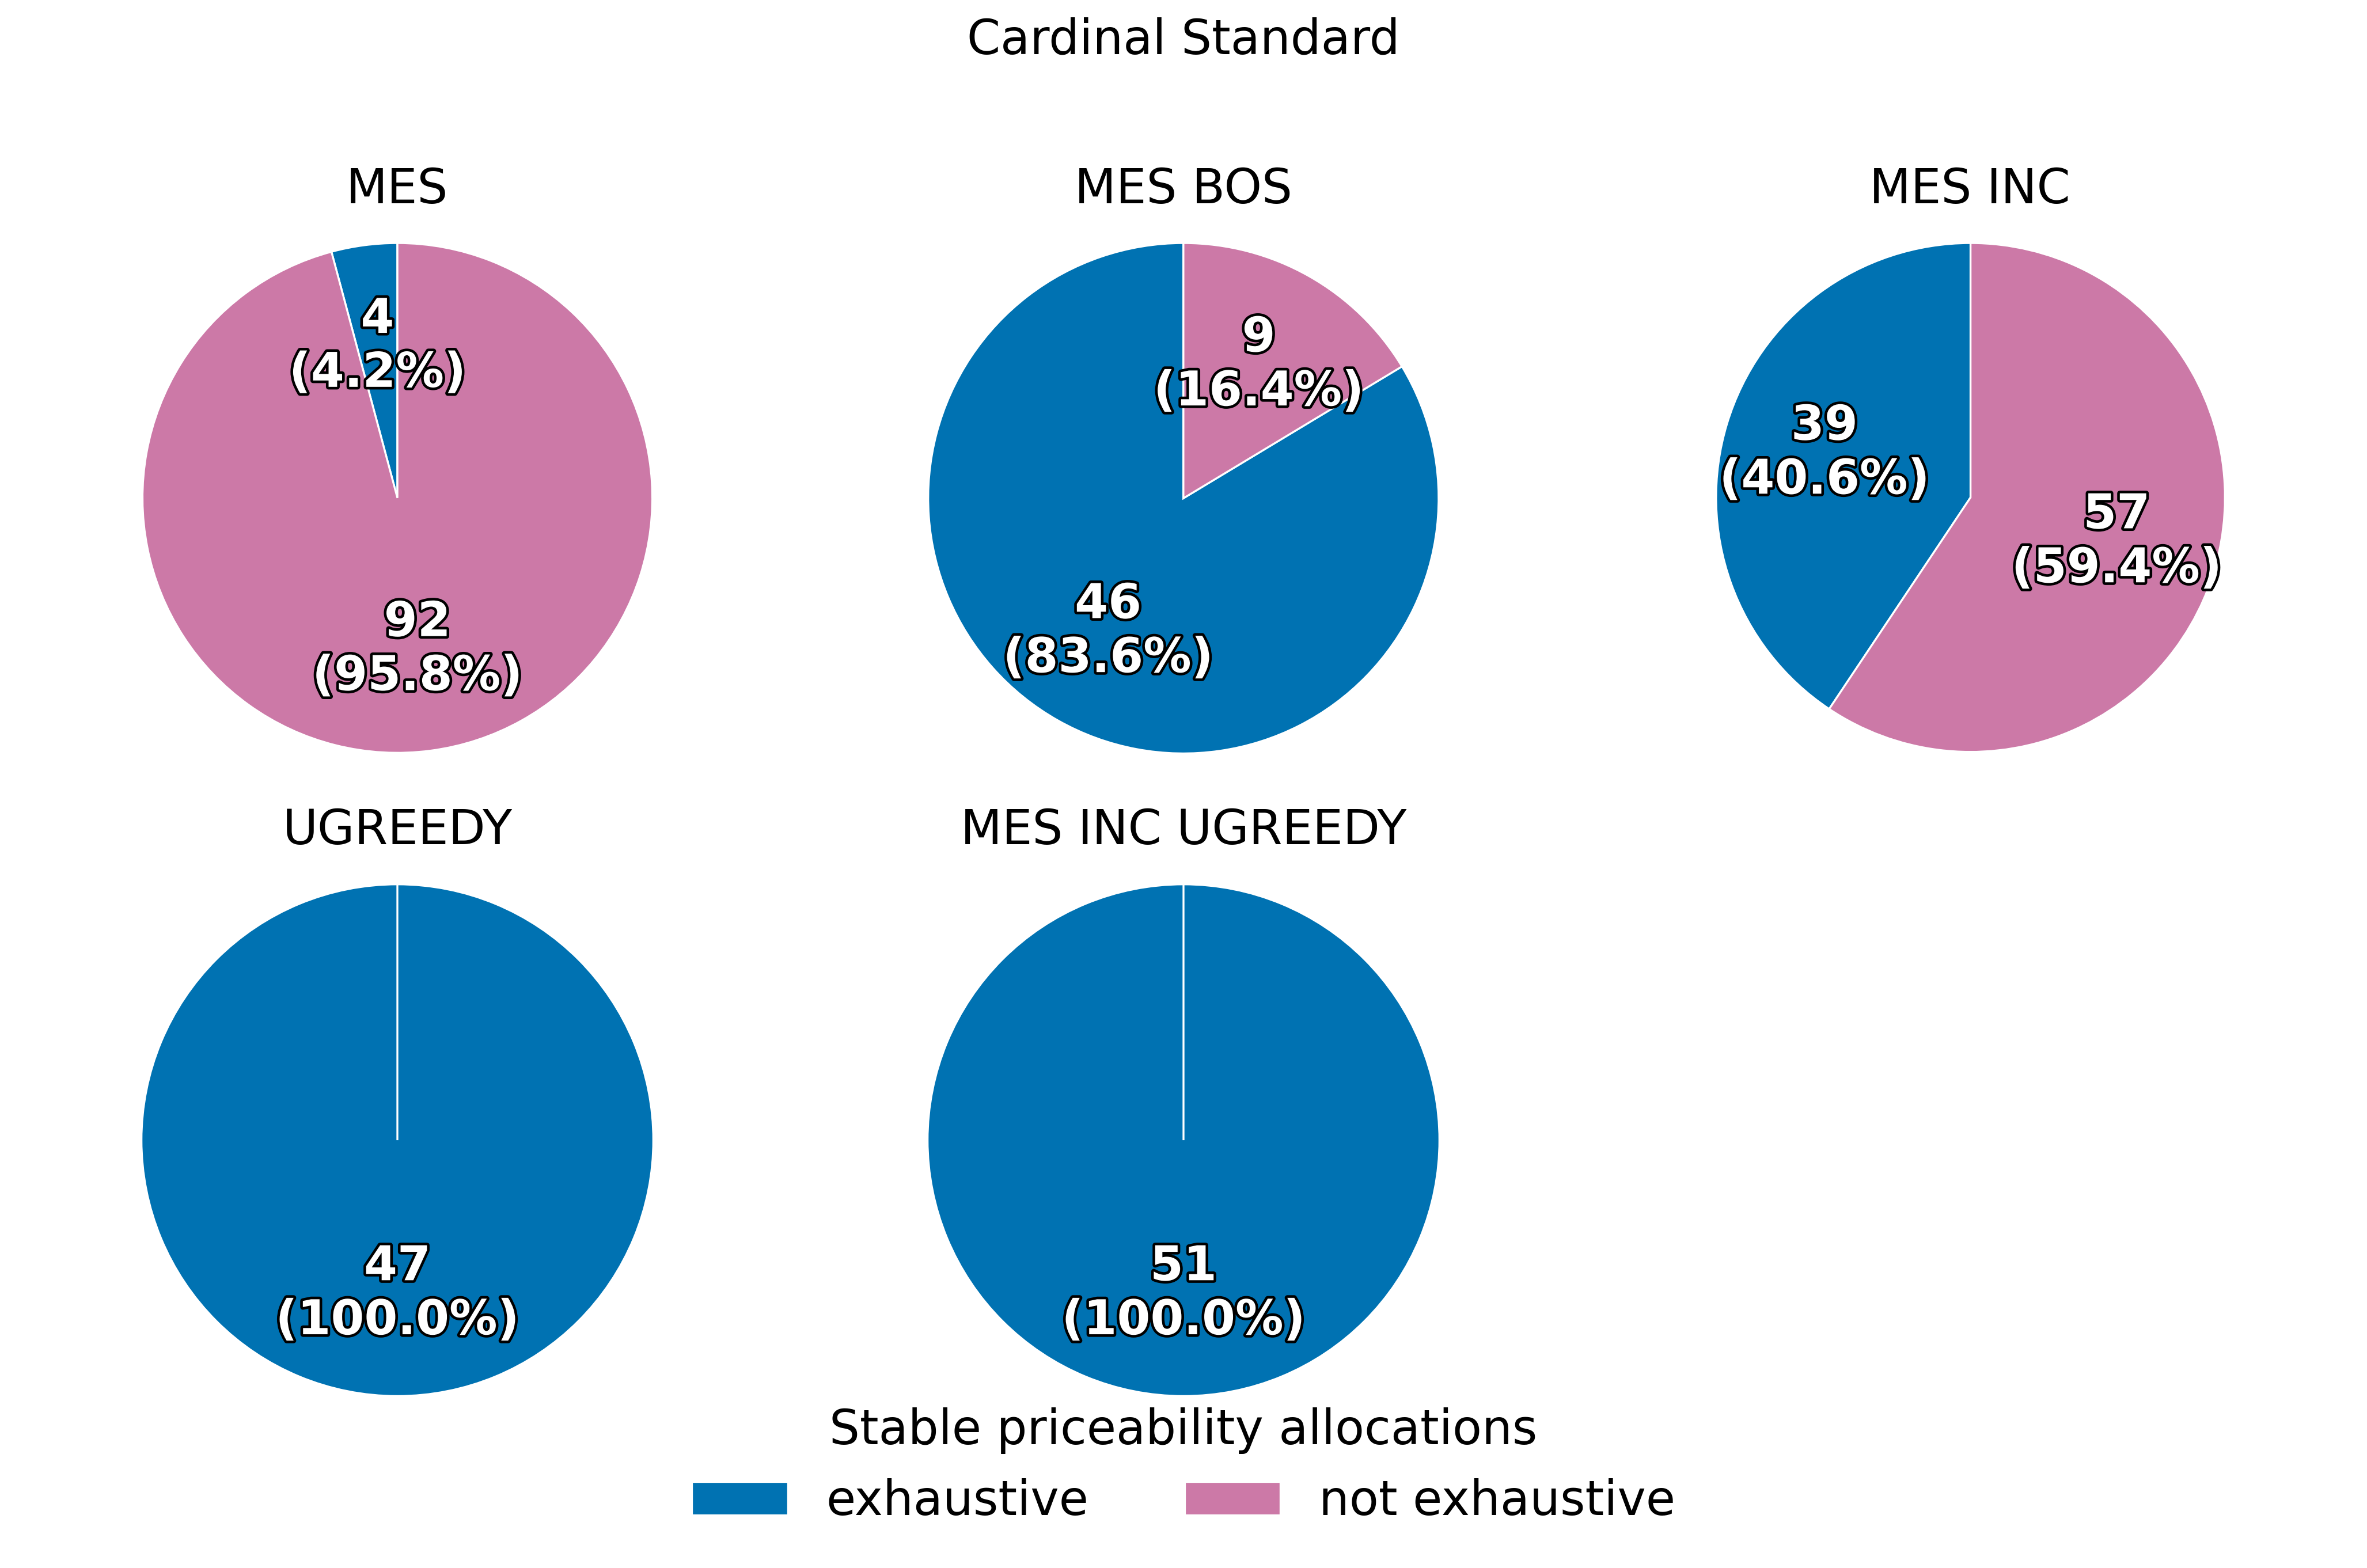
\includegraphics[width=0.7\textwidth]{figures/plots/cardinal-standard/cardinal_standard_stability_pies.png}
  \caption{Percentage of stable priceable allocations being exhaustive for cardinal-based ballots.}
  \label{fig:myplot}
\end{figure}

\begin{figure}[H]         
  \centering              
  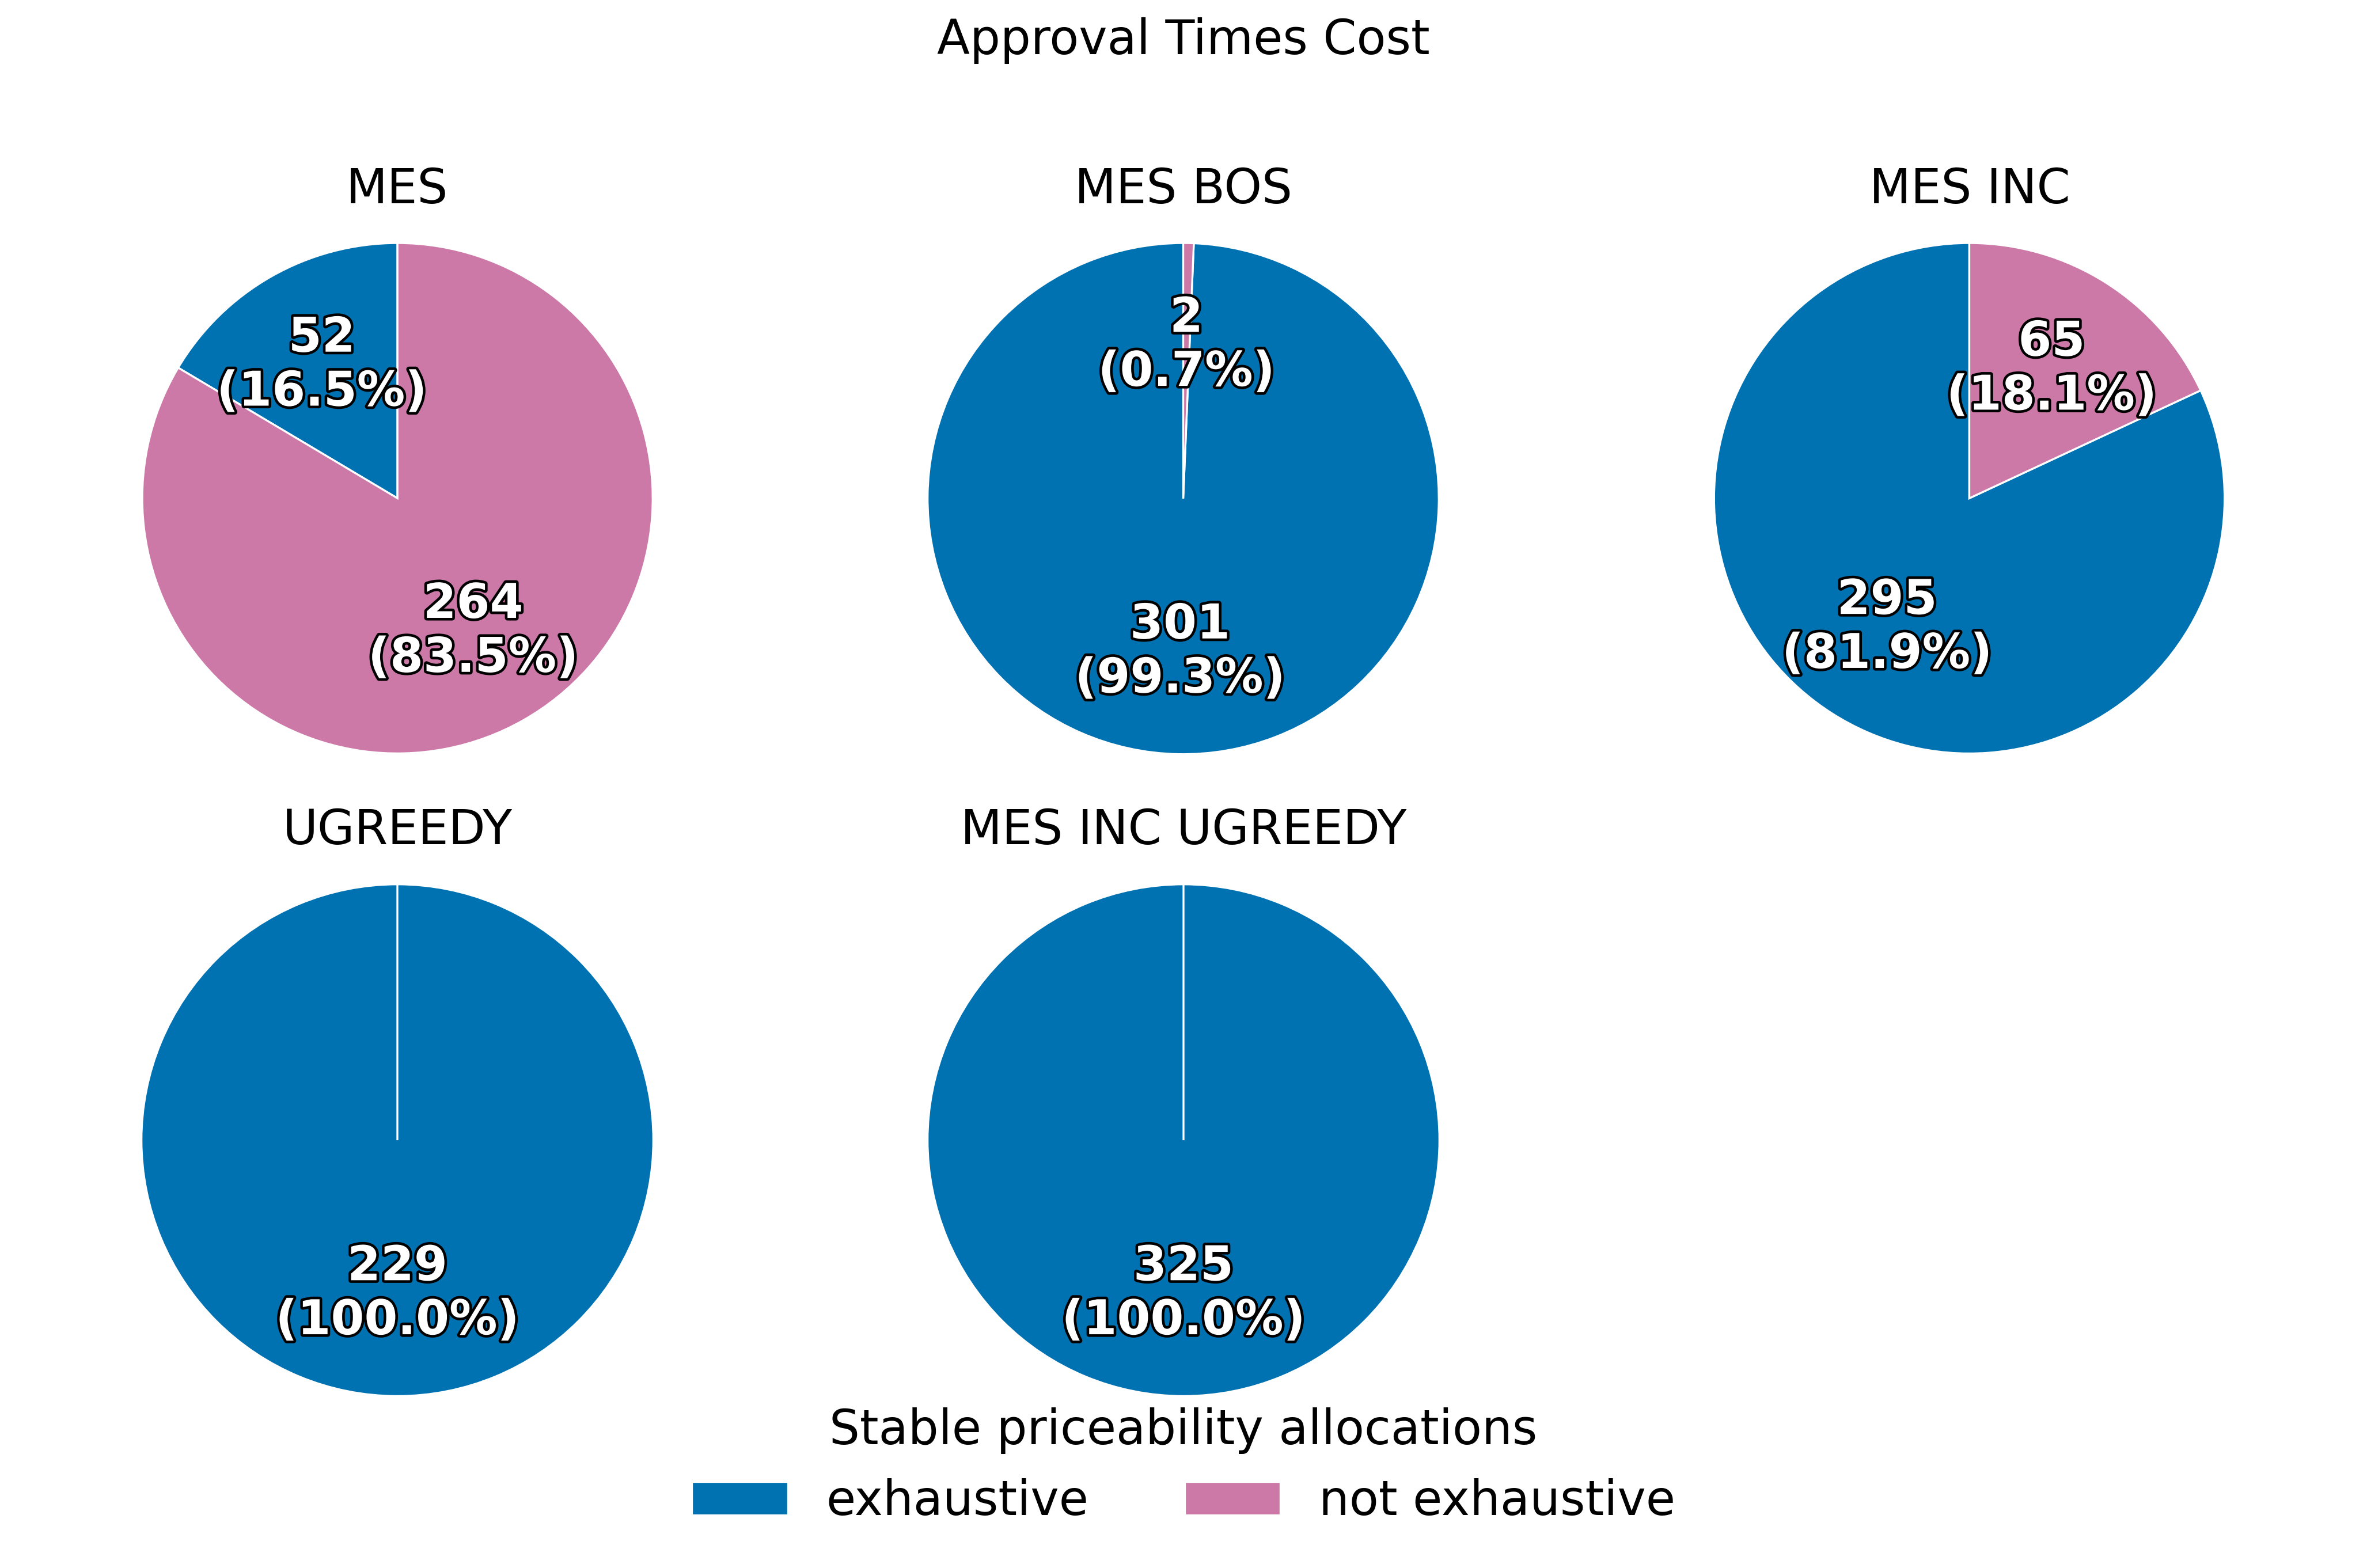
\includegraphics[width=0.7\textwidth]{figures/plots/approval-times-cost/approval_times_cost_stability_pies.png}
  \caption{Percentage of stable priceable allocations being exhaustive for approval-based ballots adjusted to cost utility.}
  \label{fig:myplot}
\end{figure}

\begin{figure}[H]         
  \centering              
  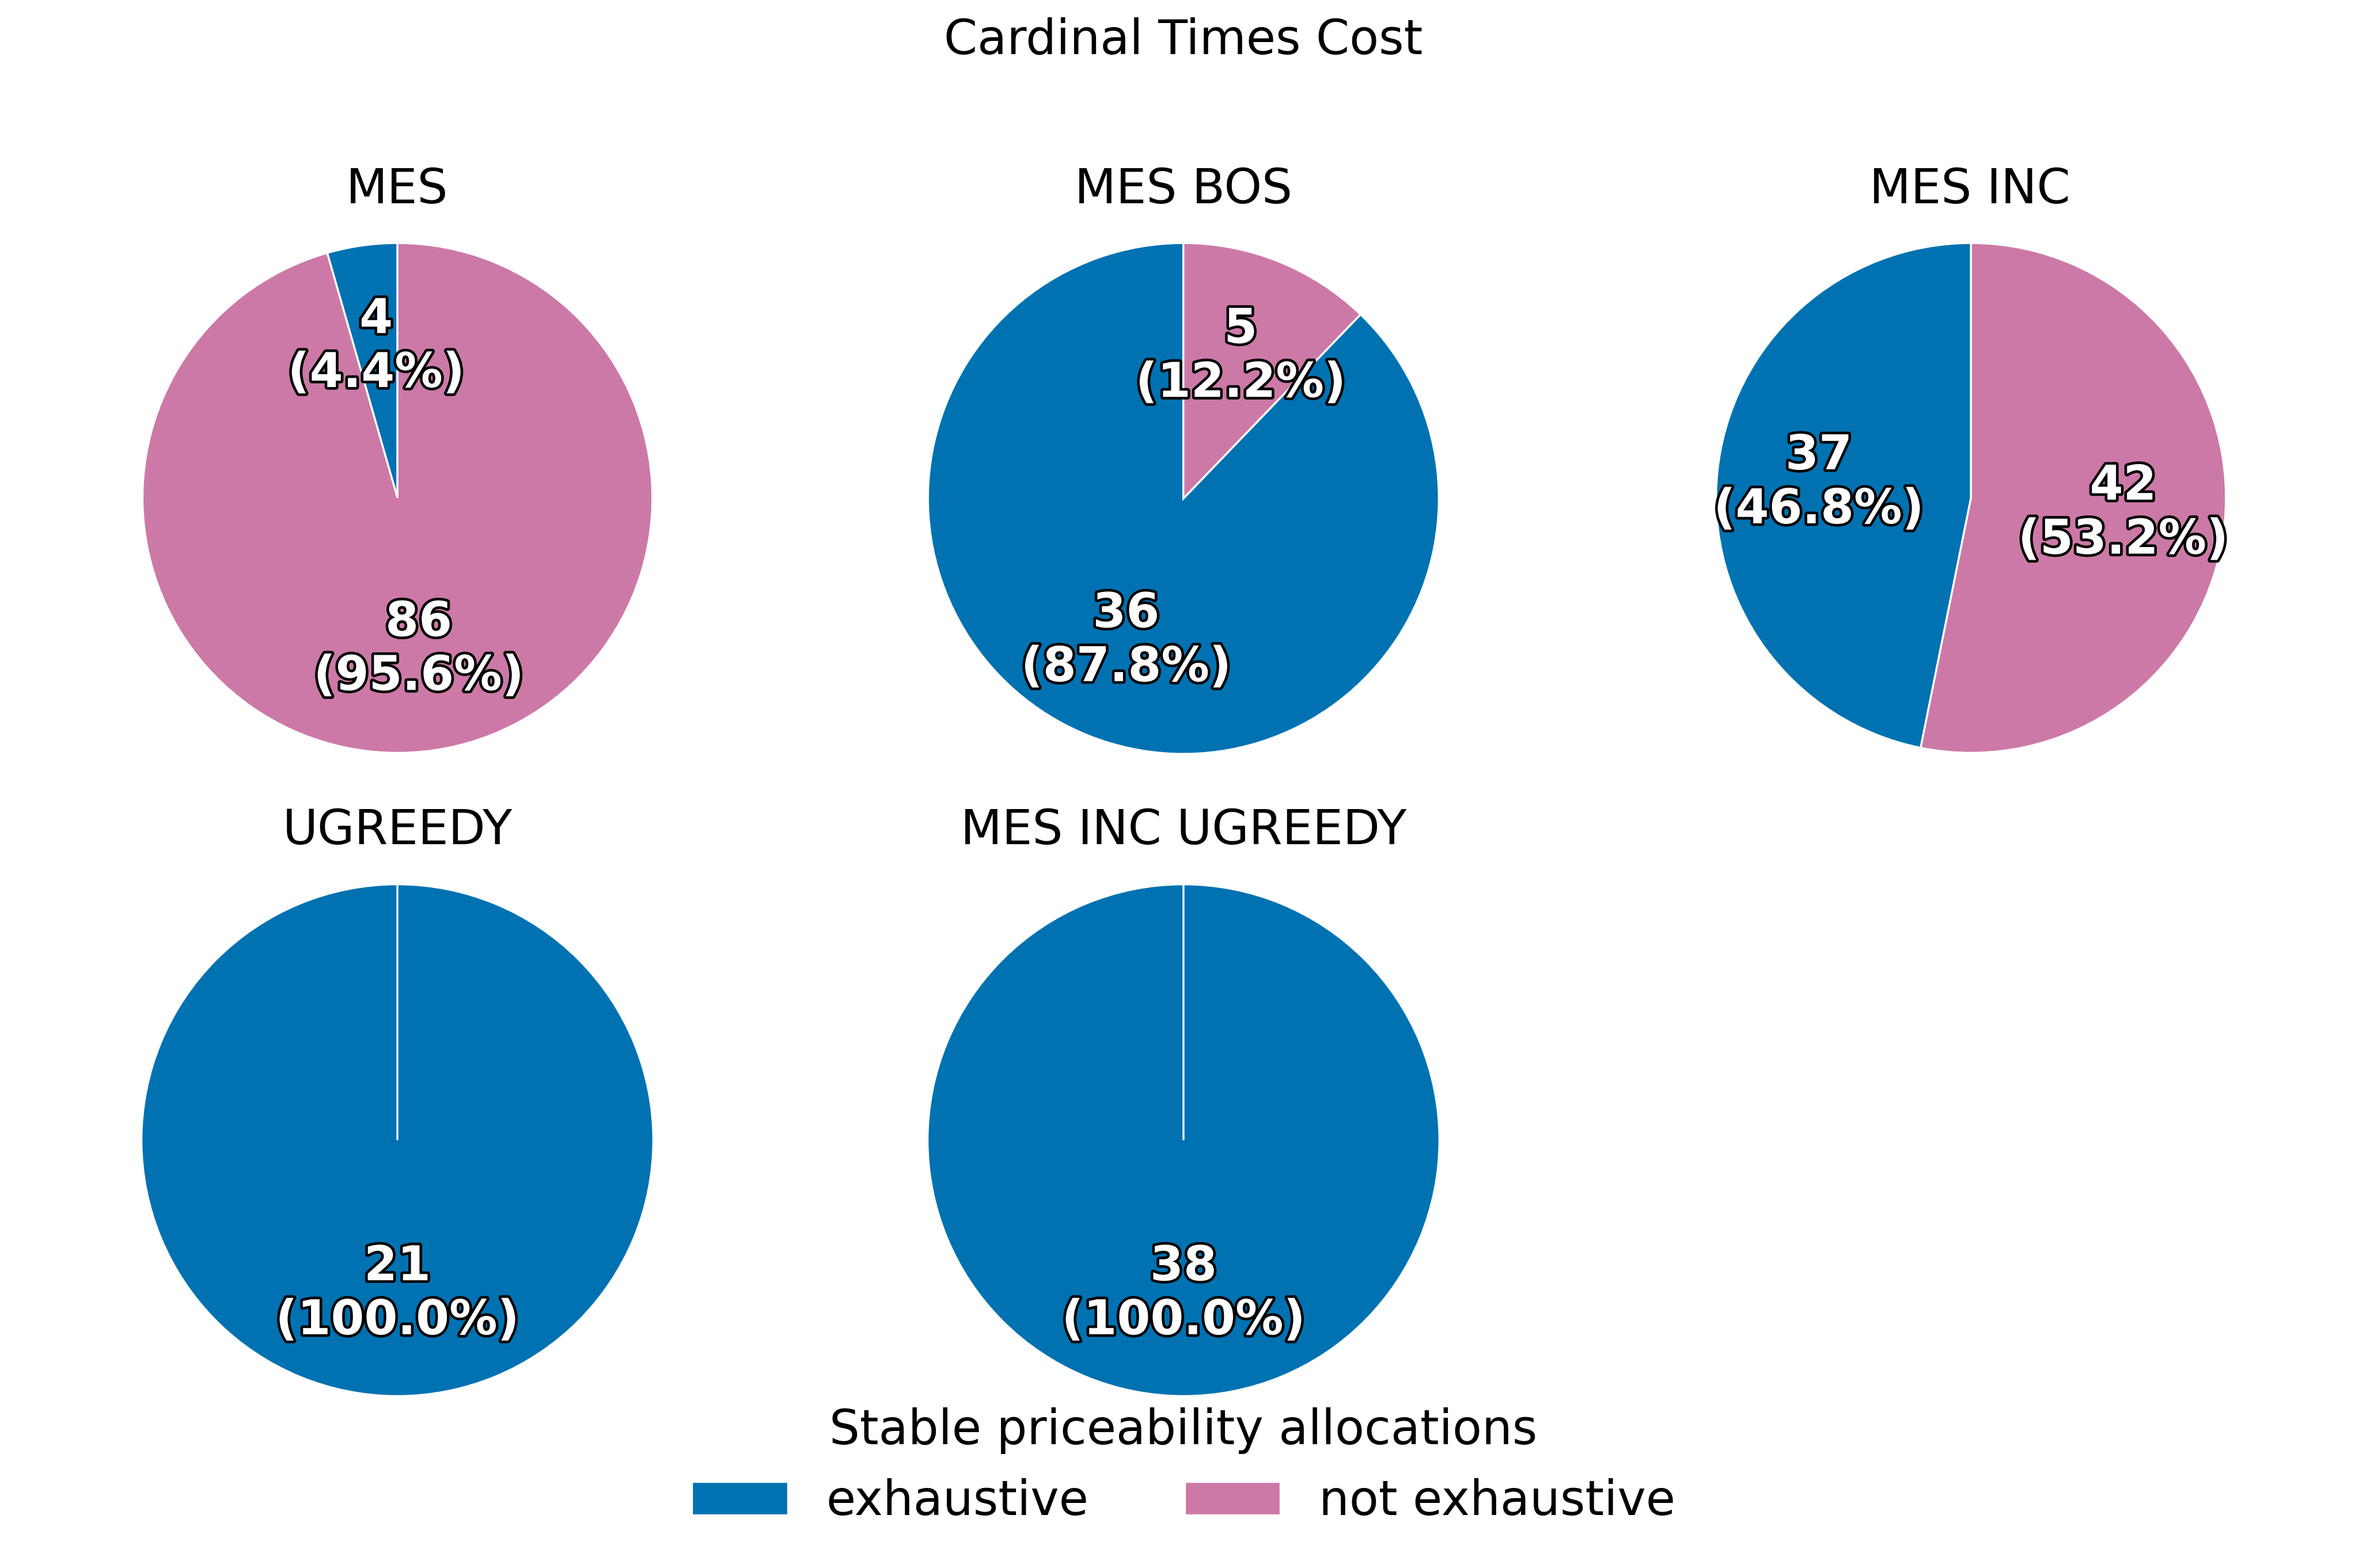
\includegraphics[width=0.7\textwidth]{figures/plots/cardinal-times-cost/cardinal_times_cost_stability_pies.png}
  \caption{Percentage of stable priceable allocations being exhaustive for cardinal-based ballots adjusted to cost utility.}
  \label{fig:myplot}
\end{figure}


Next, we look at each kind of election and check if any of the election rules used in empirical evaluation is able to find a stable-priceable or a priceable solution.

\begin{figure}[H]         
  \centering              
  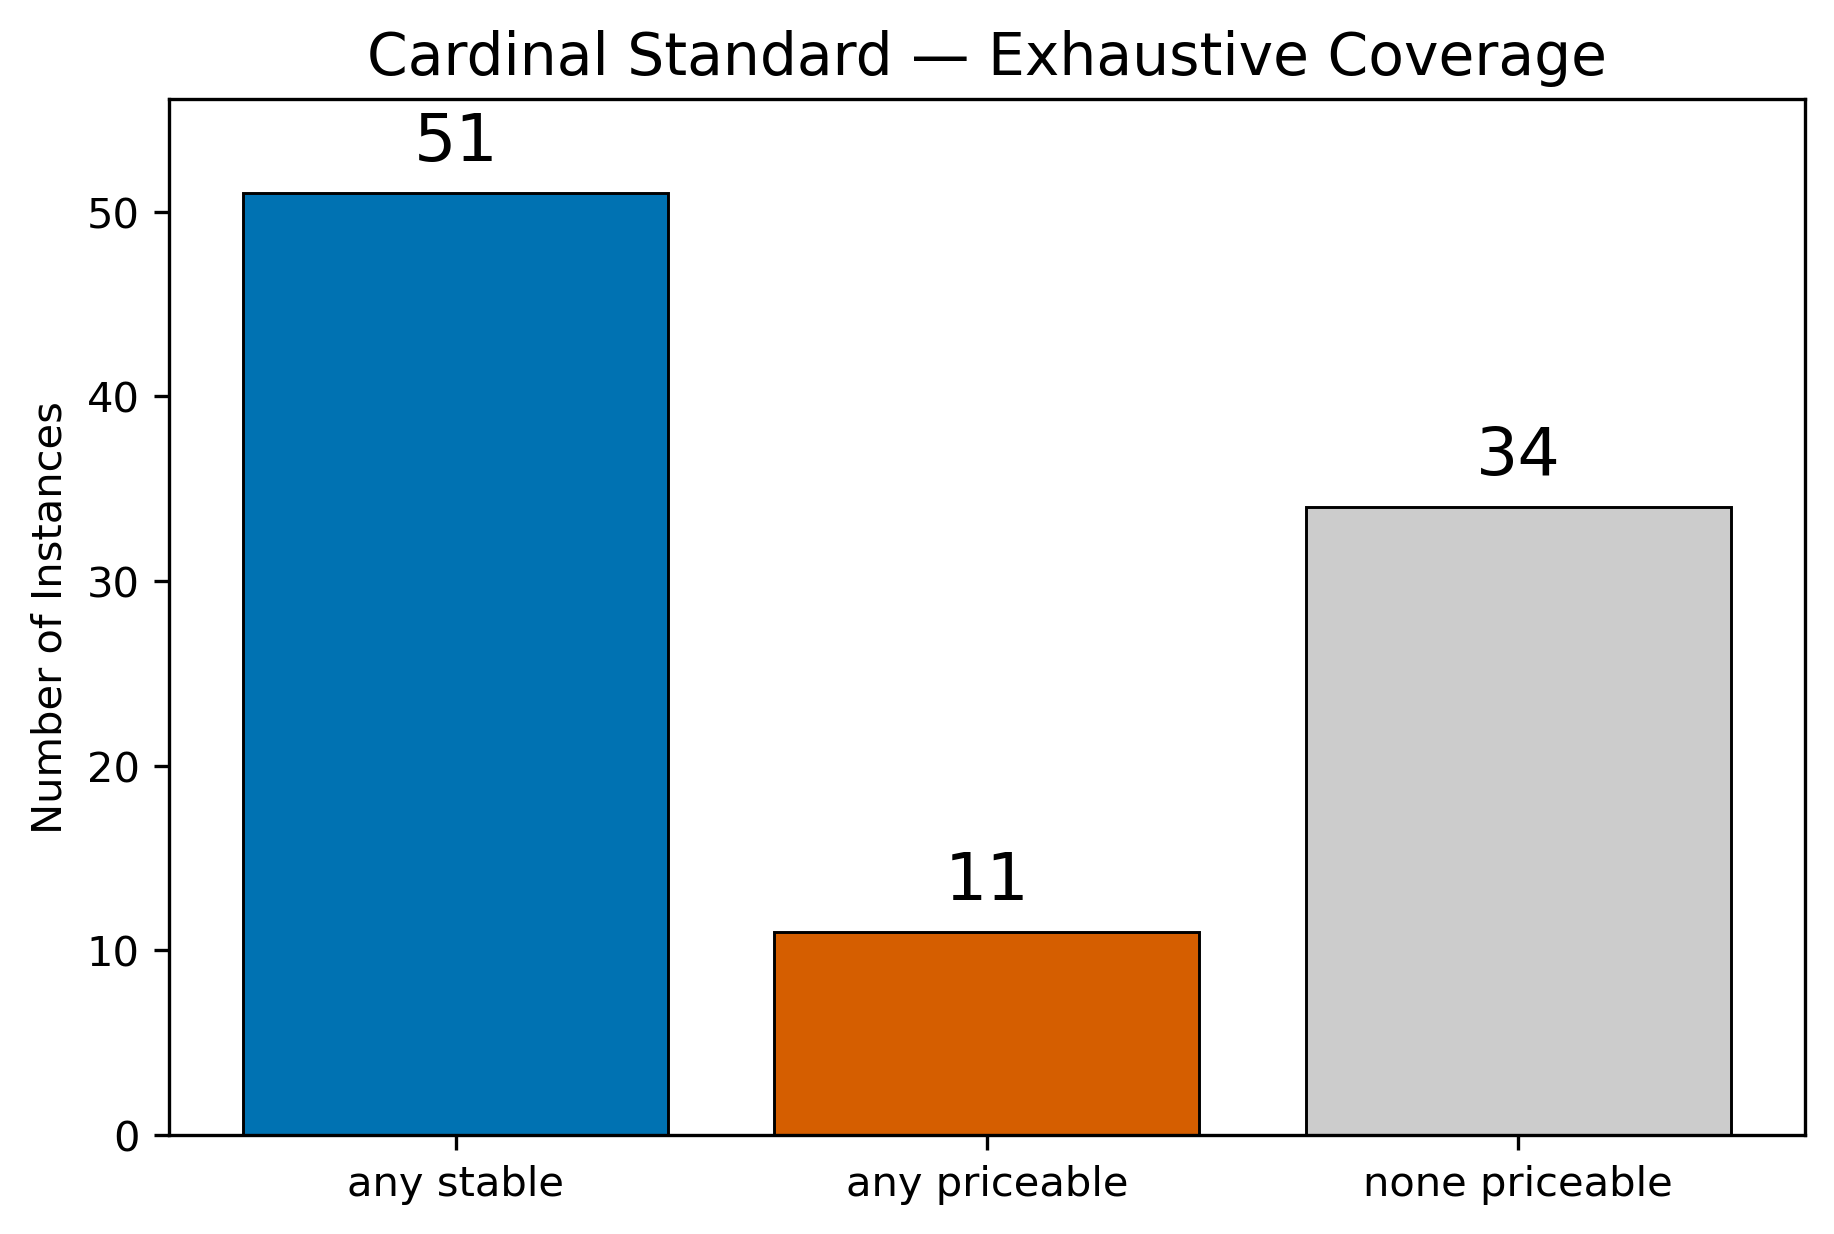
\includegraphics[width=0.7\textwidth]{figures/plots/cardinal-standard/cardinal_standard_coverage_exhaustive.png}
  \caption{Number of instances of standard cardinal-based elections, where at least one method return an exhaustive stable priceable or priceable allocation.}
  \label{fig:myplot}
\end{figure}
\begin{figure}[H]         
  \centering              
  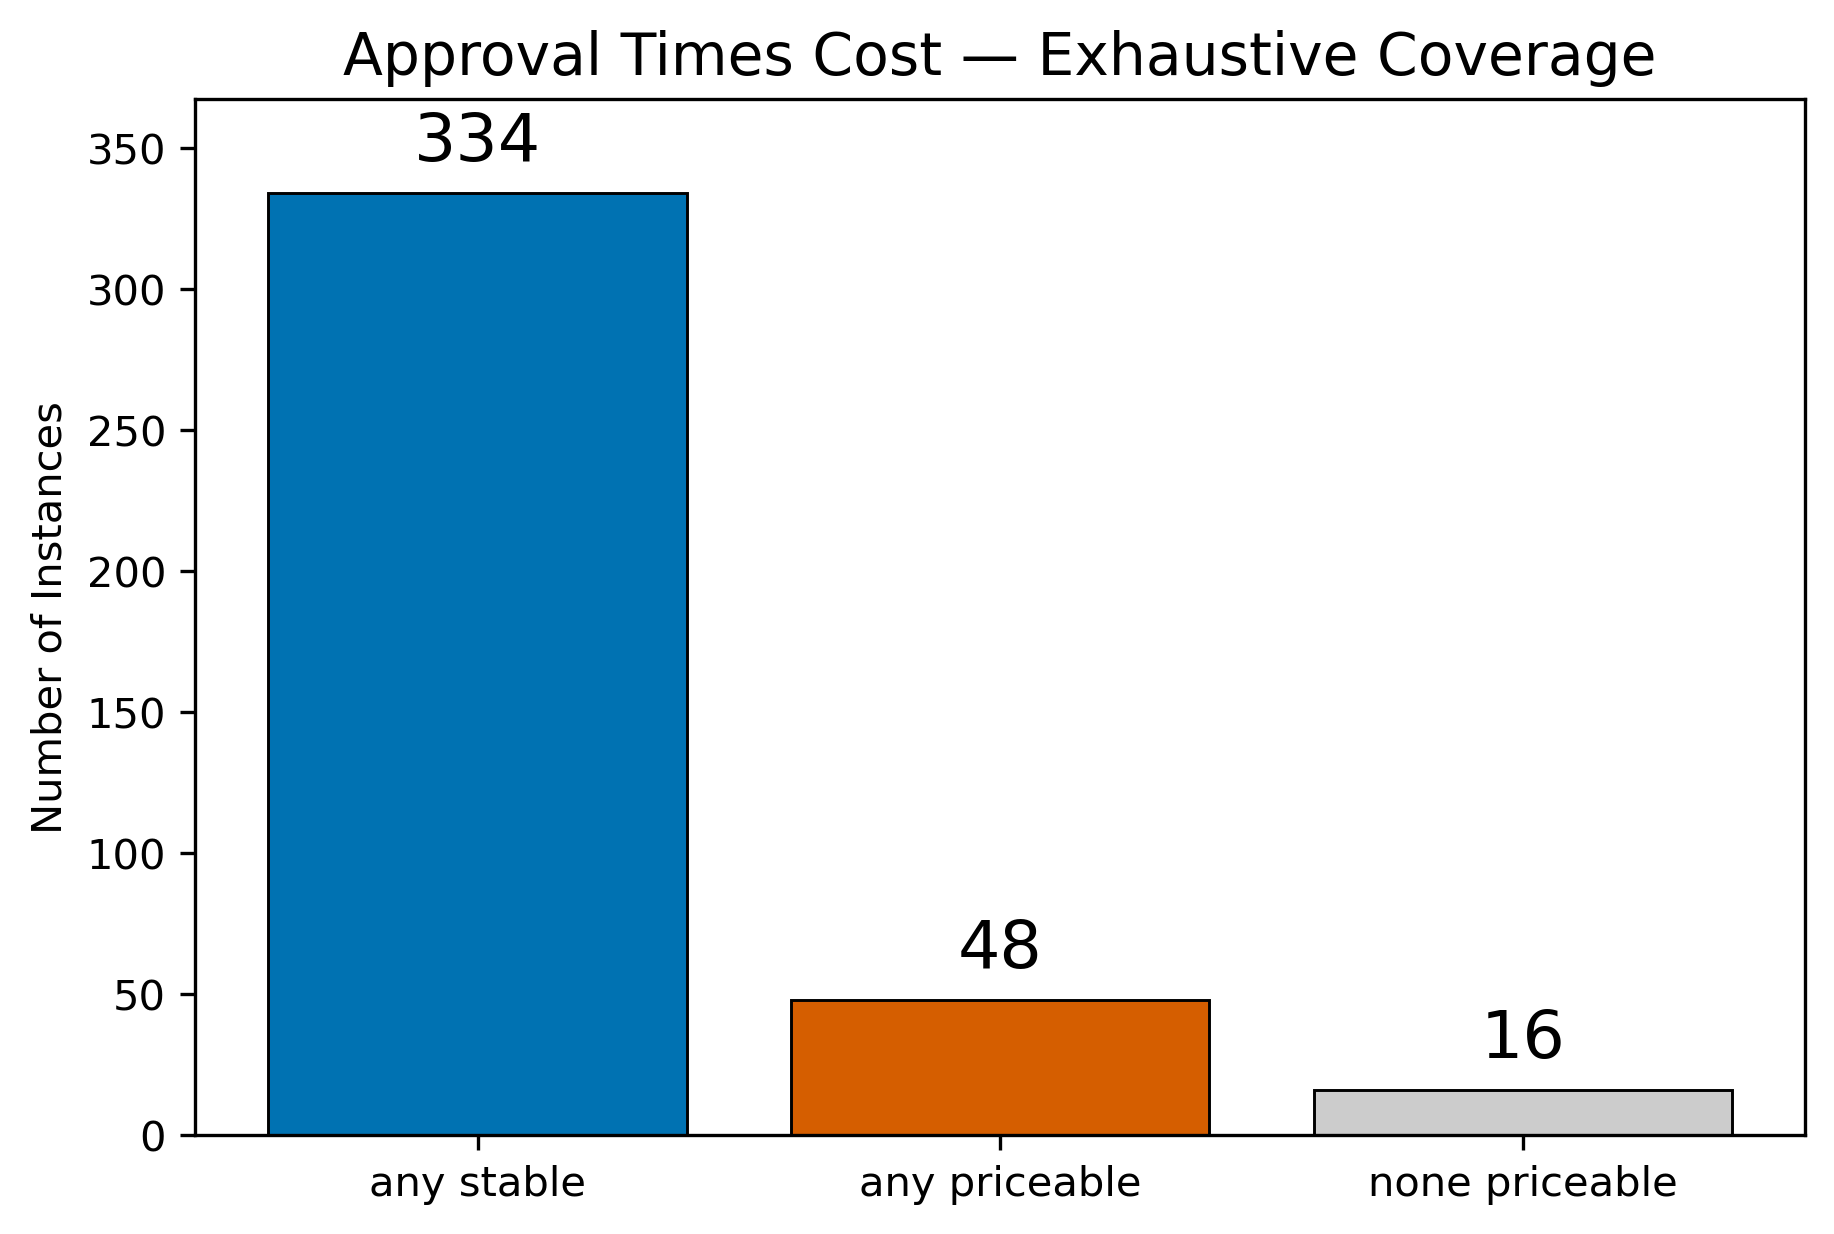
\includegraphics[width=0.7\textwidth]{figures/plots/approval-times-cost/approval_times_cost_coverage_exhaustive.png}
  \caption{Number of instances of standard approval-based cost-adjusted elections, where at least one method return an exhaustive stable priceable or priceable allocation.}
  \label{fig:myplot}
\end{figure}
\begin{figure}[H]         
  \centering              
  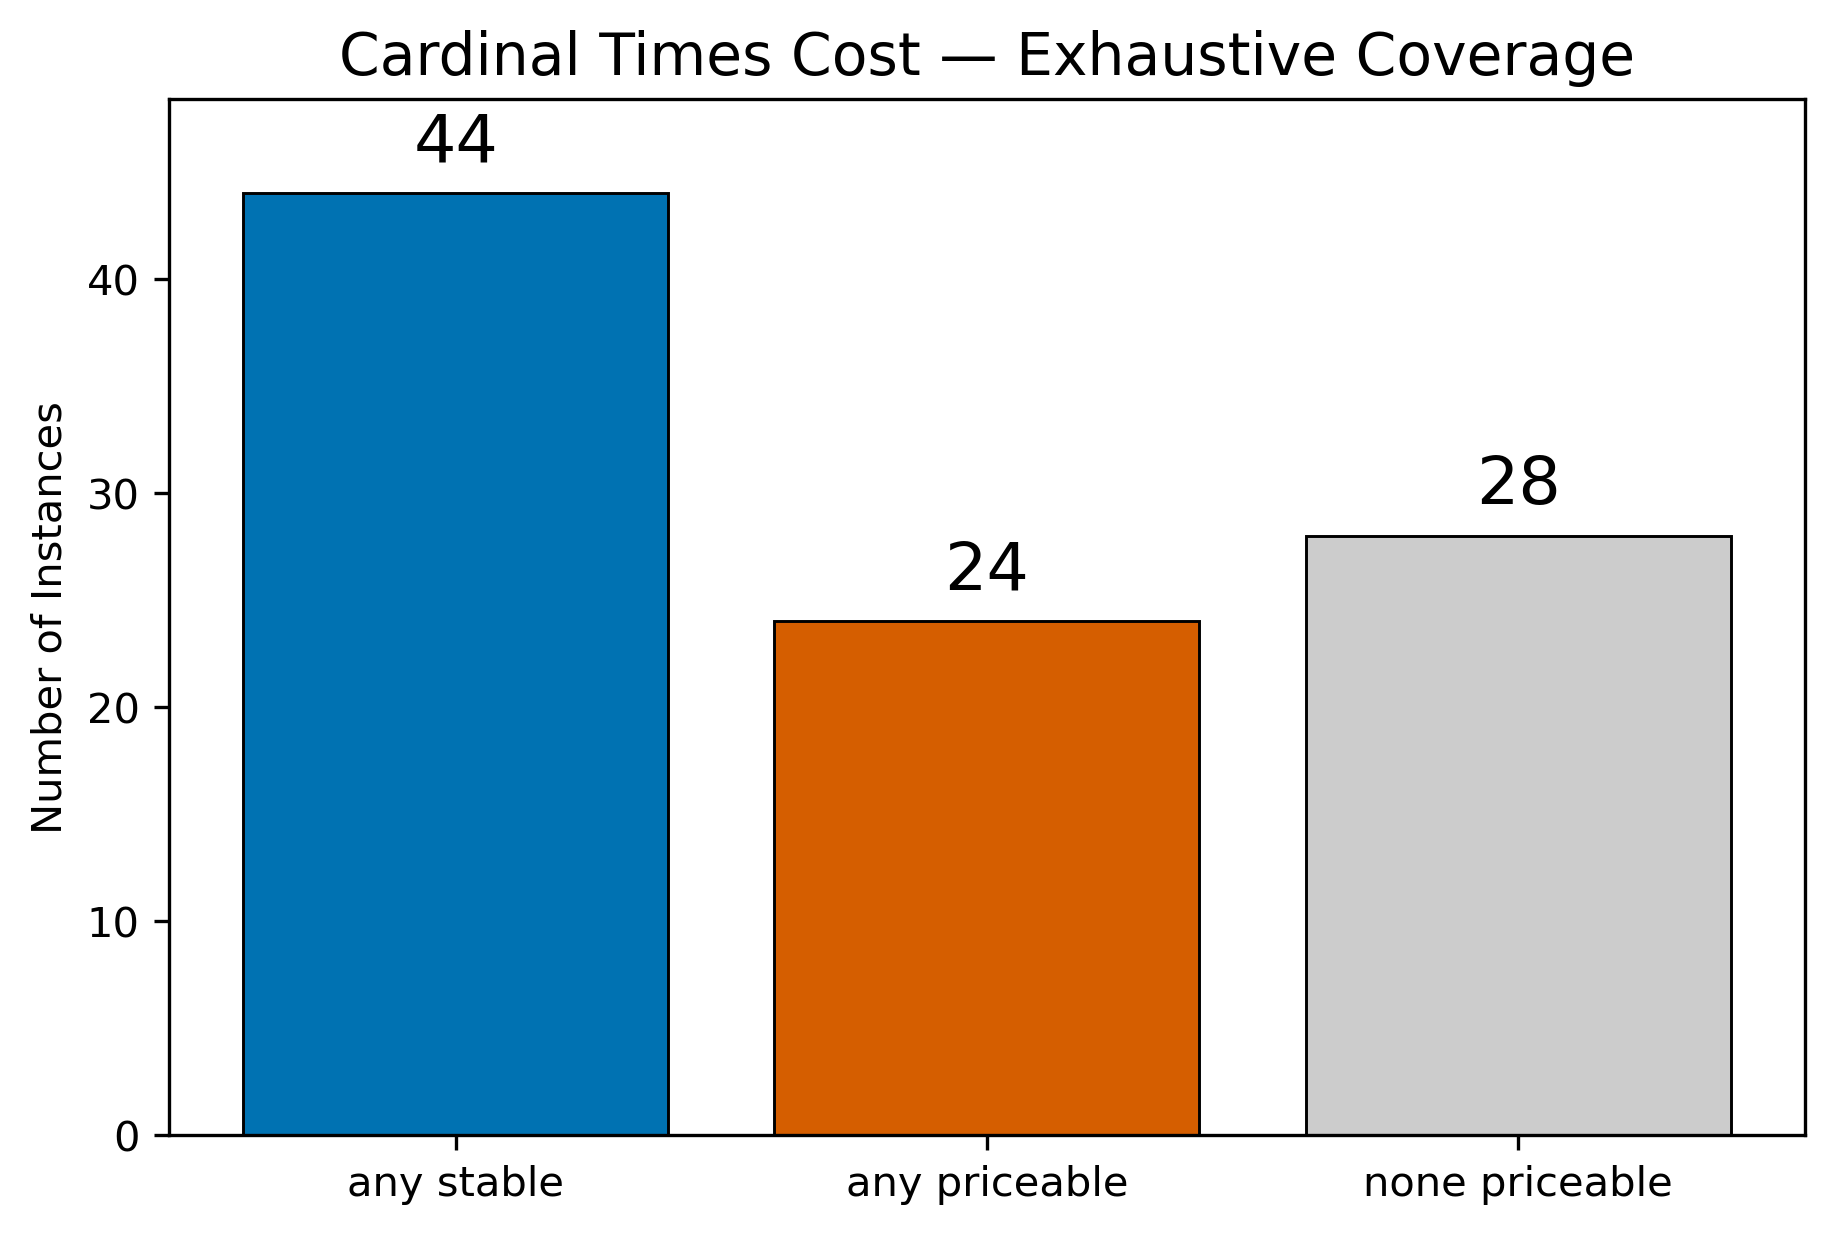
\includegraphics[width=0.7\textwidth]{figures/plots/cardinal-times-cost/cardinal_times_cost_coverage_exhaustive.png}
  \caption{Number of instances of standard cardinal-based cost-adjusted elections, where at least one method return an exhaustive stable priceable or priceable allocation.}  \label{fig:myplot}
\end{figure}
We observe that, again, the best results are by far for approval-based elections. There, at least $1$ method returns a perfect allocation in $83\%$ of elections, compared to only about $50\%$ for cardinal-based cases, regardless of the application of cost utility. All methods collectively tend to perform significantly worse when working with cardinal ballots.

However, it does not necessarily mean, that for the elections where none of the tested election rules provide exhaustive priceable or stable priceable elections, the election rules behave poorly. As we are aware of election instances, where no outcome is priceable while exhaustive, we check in how many cases the tested methods failed to find existing allocations satisfying the criteria. 
\begin{figure}[H]         
  \centering              
  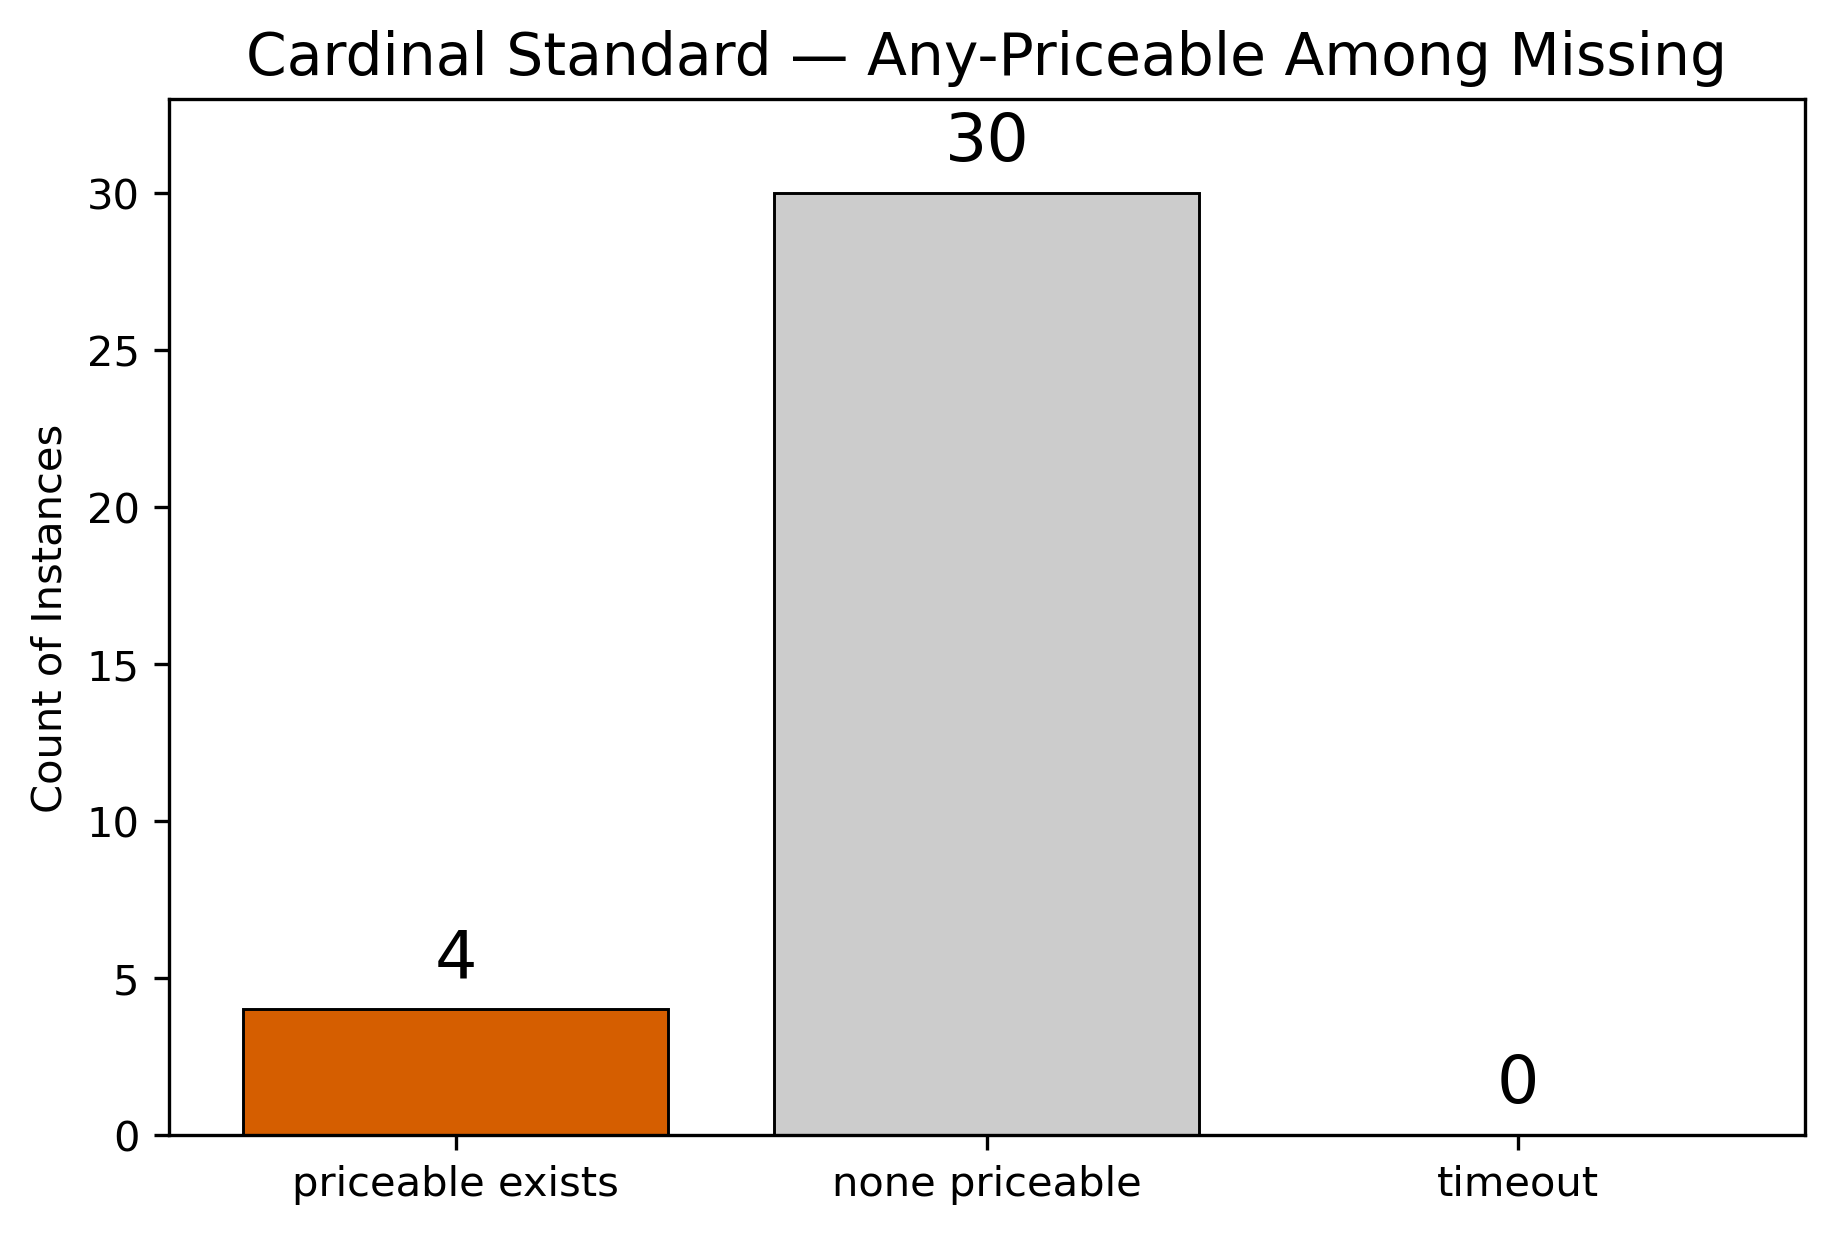
\includegraphics[width=0.7\textwidth]{figures/plots/cardinal-standard/cardinal_standard_any_priceable.png}
  \caption{Number of instances, for which no method found exhaustive priceable solution, where such solution a exists or does not, for cardinal-based elections with additive score utilities.}
  \label{fig:myplot}
\end{figure}
\begin{figure}[H]         
  \centering              
  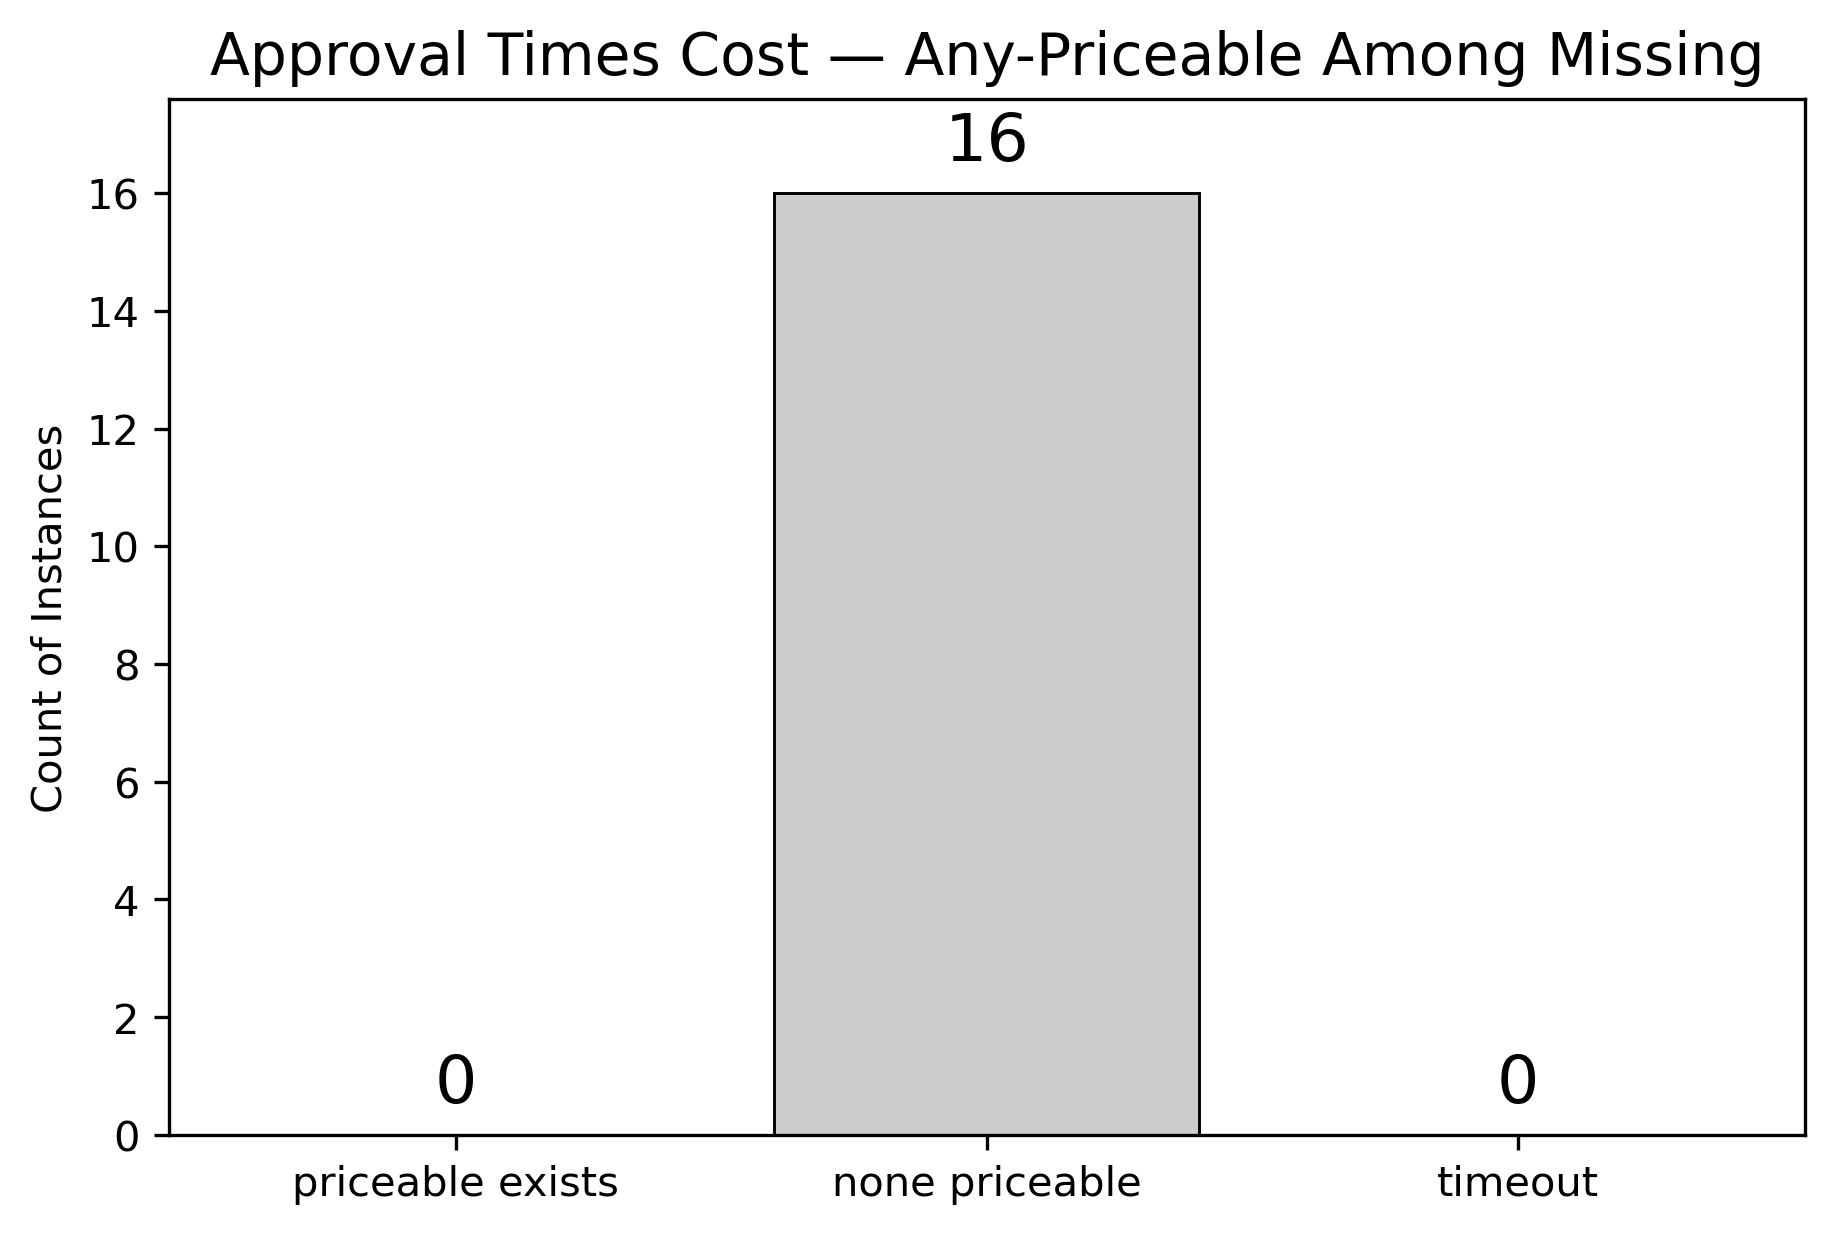
\includegraphics[width=0.7\textwidth]{figures/plots/approval-times-cost/approval_times_cost_any_priceable.png}
  \caption{Number of instances, for which no method found exhaustive priceable solution, where such a solution exists or does not, for approval-based elections with cost utilities.}
  \label{fig:myplot}
\end{figure}
\begin{figure}[H]         
  \centering              
  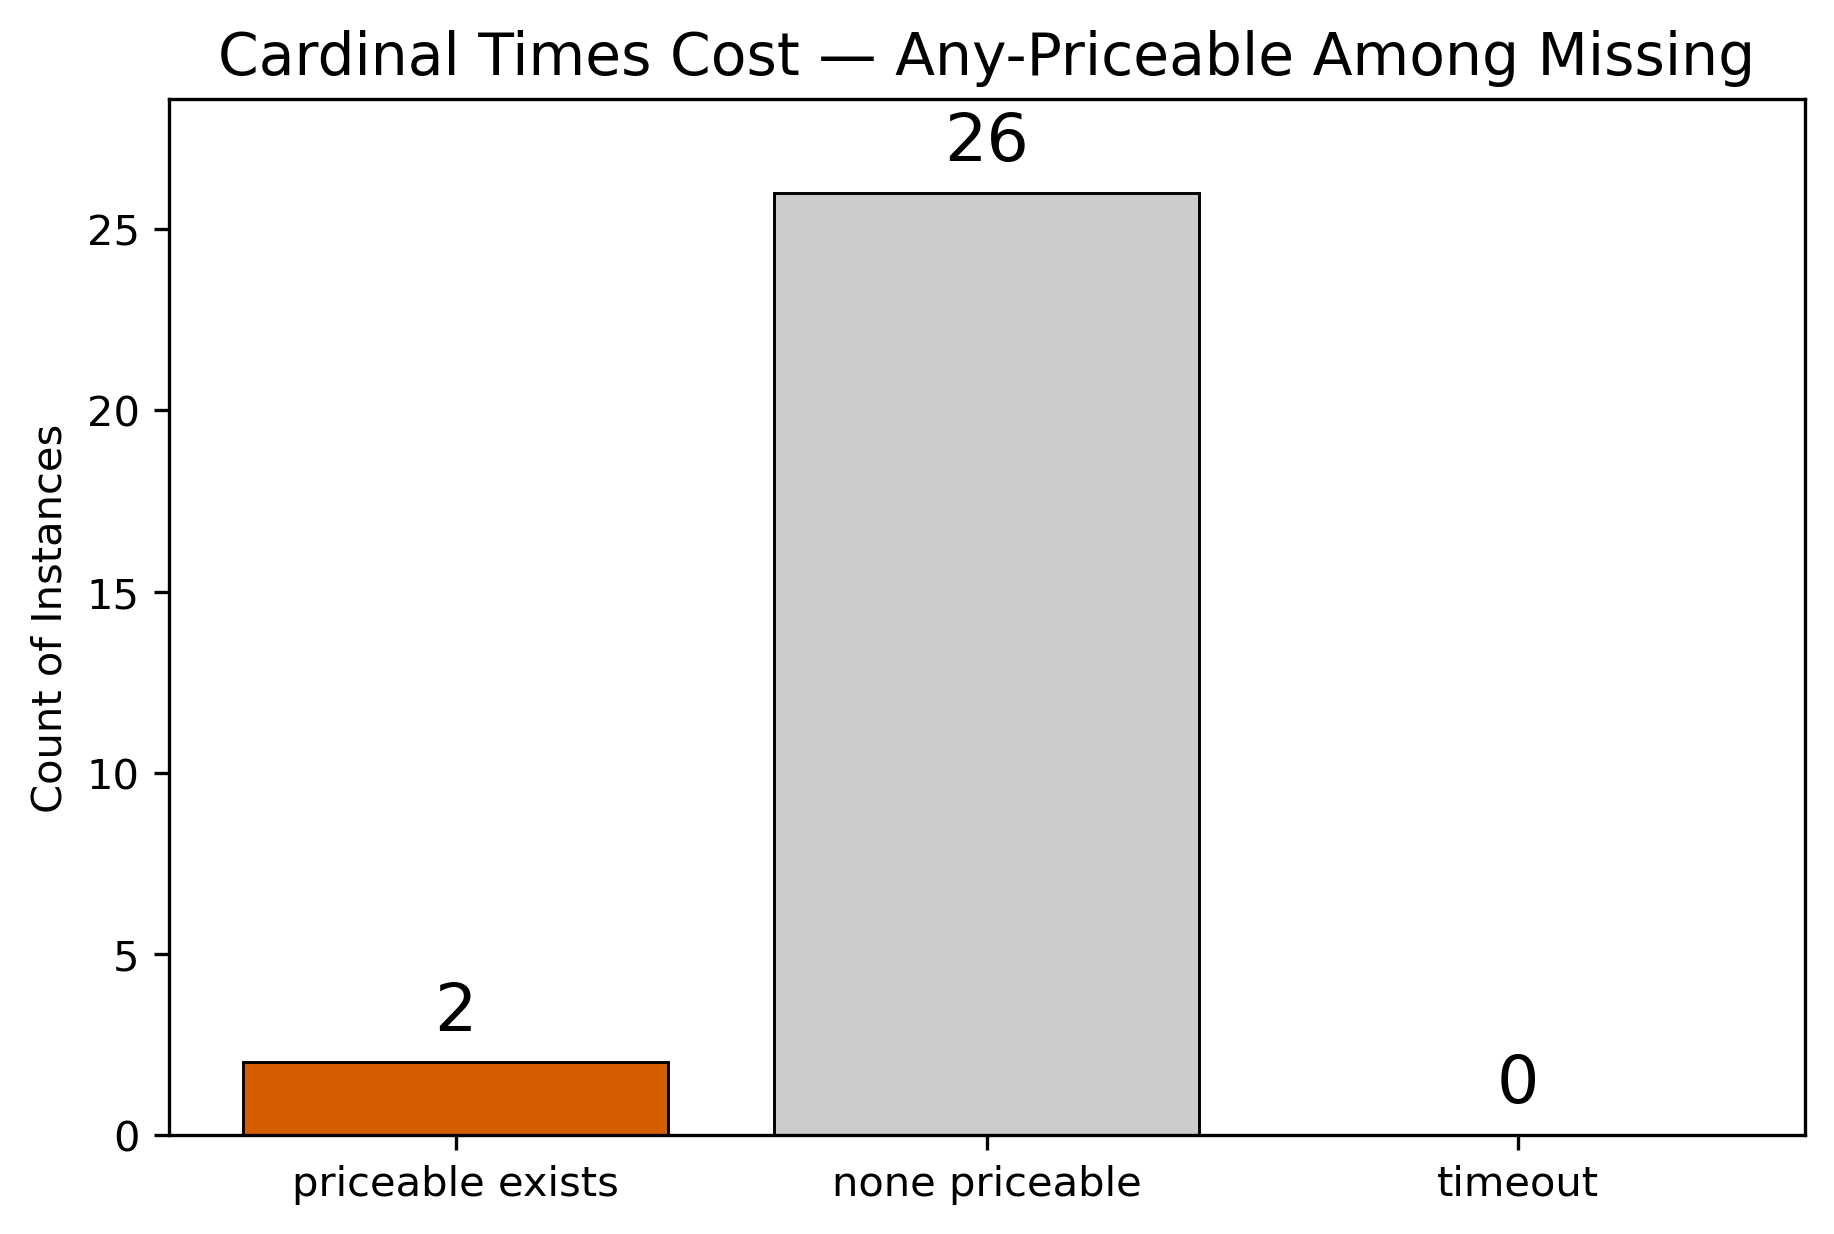
\includegraphics[width=0.7\textwidth]{figures/plots/cardinal-times-cost/cardinal_times_cost_any_priceable.png}
  \caption{Number of instances, for which no method found exhaustive priceable solution, where such a solution exists or does not, for cardinal-based elections with cost utilities.}
  \label{fig:myplot}
\end{figure}
It turns out, that depending on the election setting and satisfaction measure, in over $90\%$ of cases where no method has found an exhaustive priceable allocation, it was because such an allocation does not exist.

Finally, we do the same analysis, but for stable priceability. We check, among the instances where all methods failed to return a stable priceable and exhaustive allocation, how many of them actually have such a solution.
\begin{figure}[H]         
  \centering              
  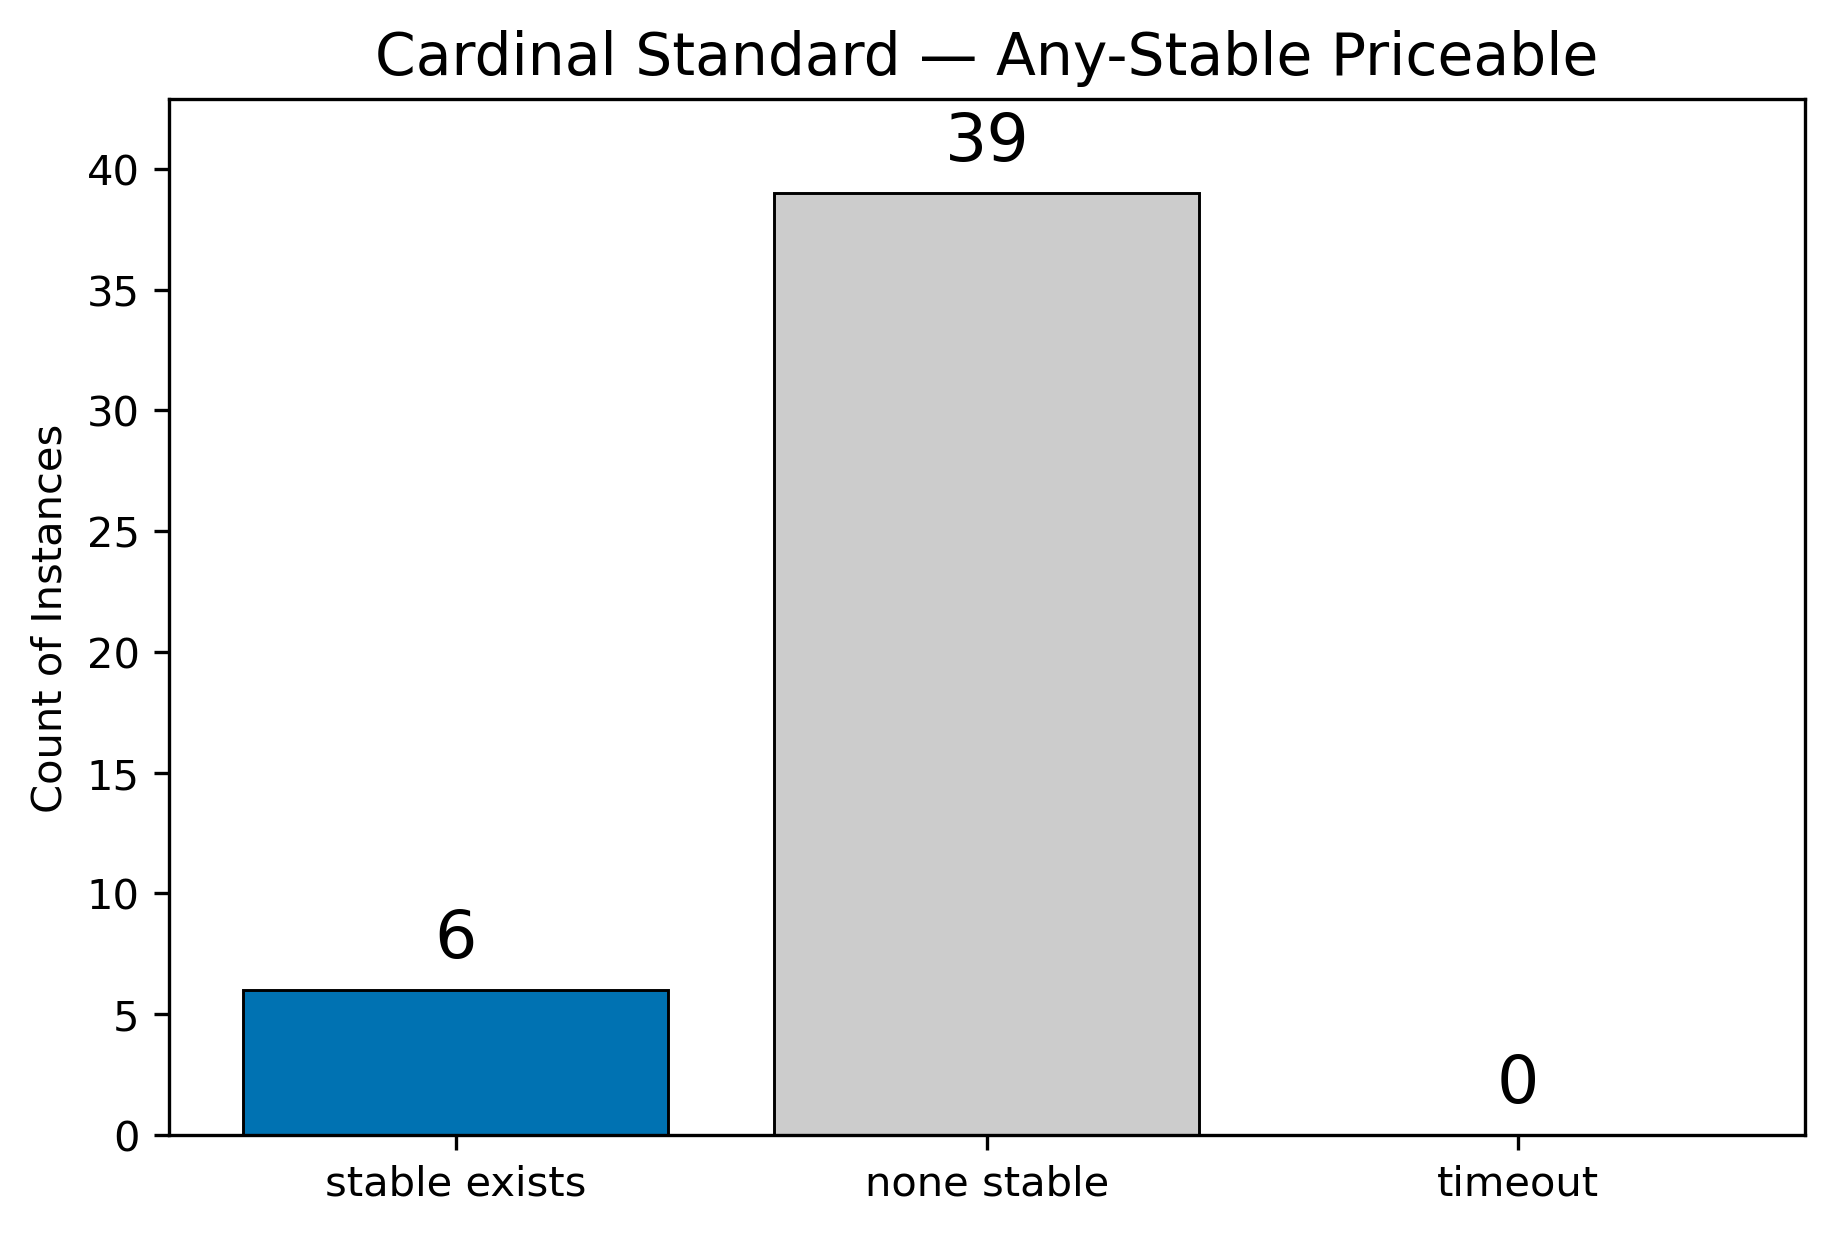
\includegraphics[width=0.7\textwidth]{figures/plots/cardinal-standard/cardinal_standard_any_stable_exhaustive.png}
  \caption{Number of instances, for which no method found exhaustive stable priceable solution, where such a solution exists or does not, for cardinal-based elections with additive score utilities.}
  \label{fig:myplot}
\end{figure}
\begin{figure}[H]         
  \centering              
  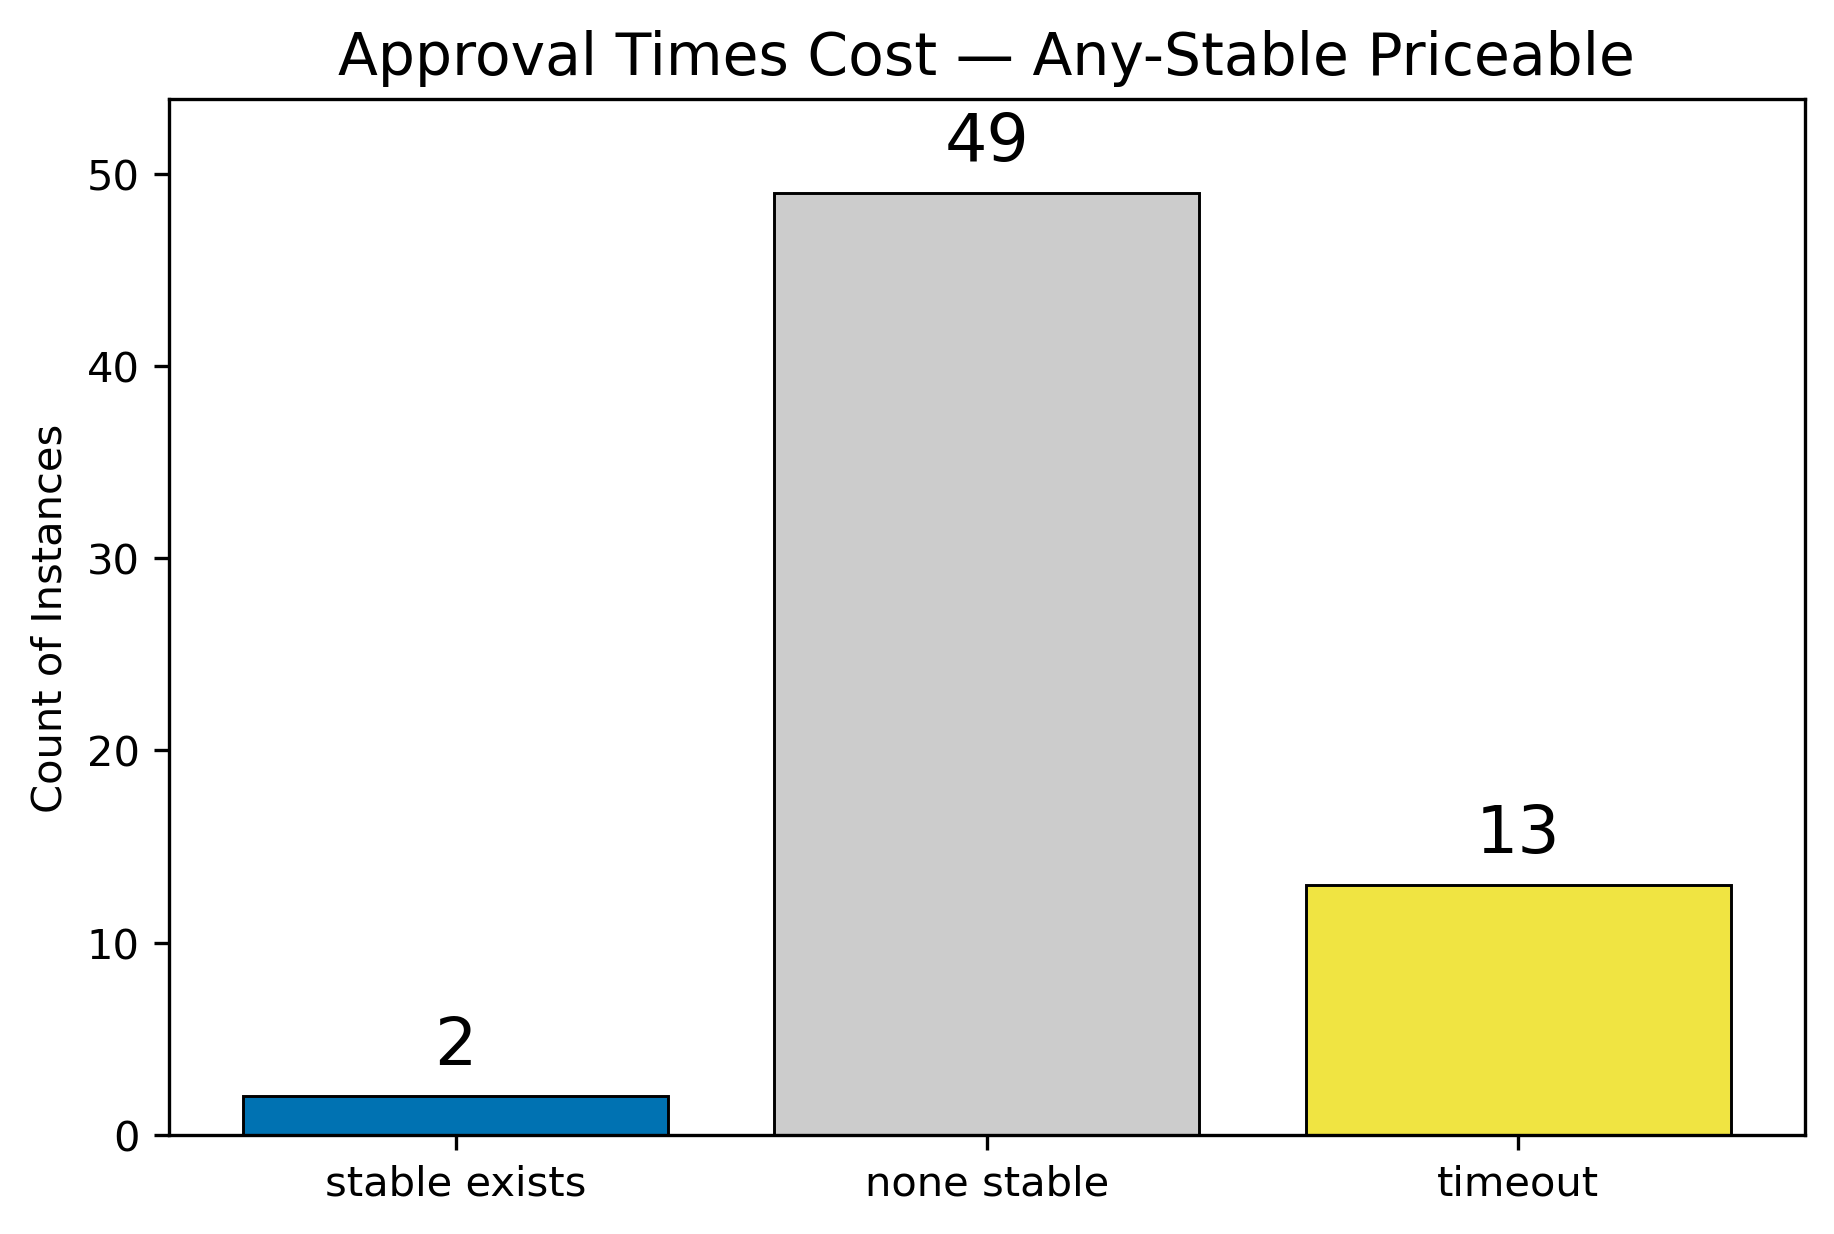
\includegraphics[width=0.7\textwidth]{figures/plots/approval-times-cost/approval_times_cost_any_stable_exhaustive.png}
  \caption{Number of instances, for which no method found exhaustive stable priceable solution, where such a solution exists or does not, for approval-based elections with cost utilities.}
  \label{fig:myplot}
\end{figure}
\begin{figure}[H]         
  \centering              
  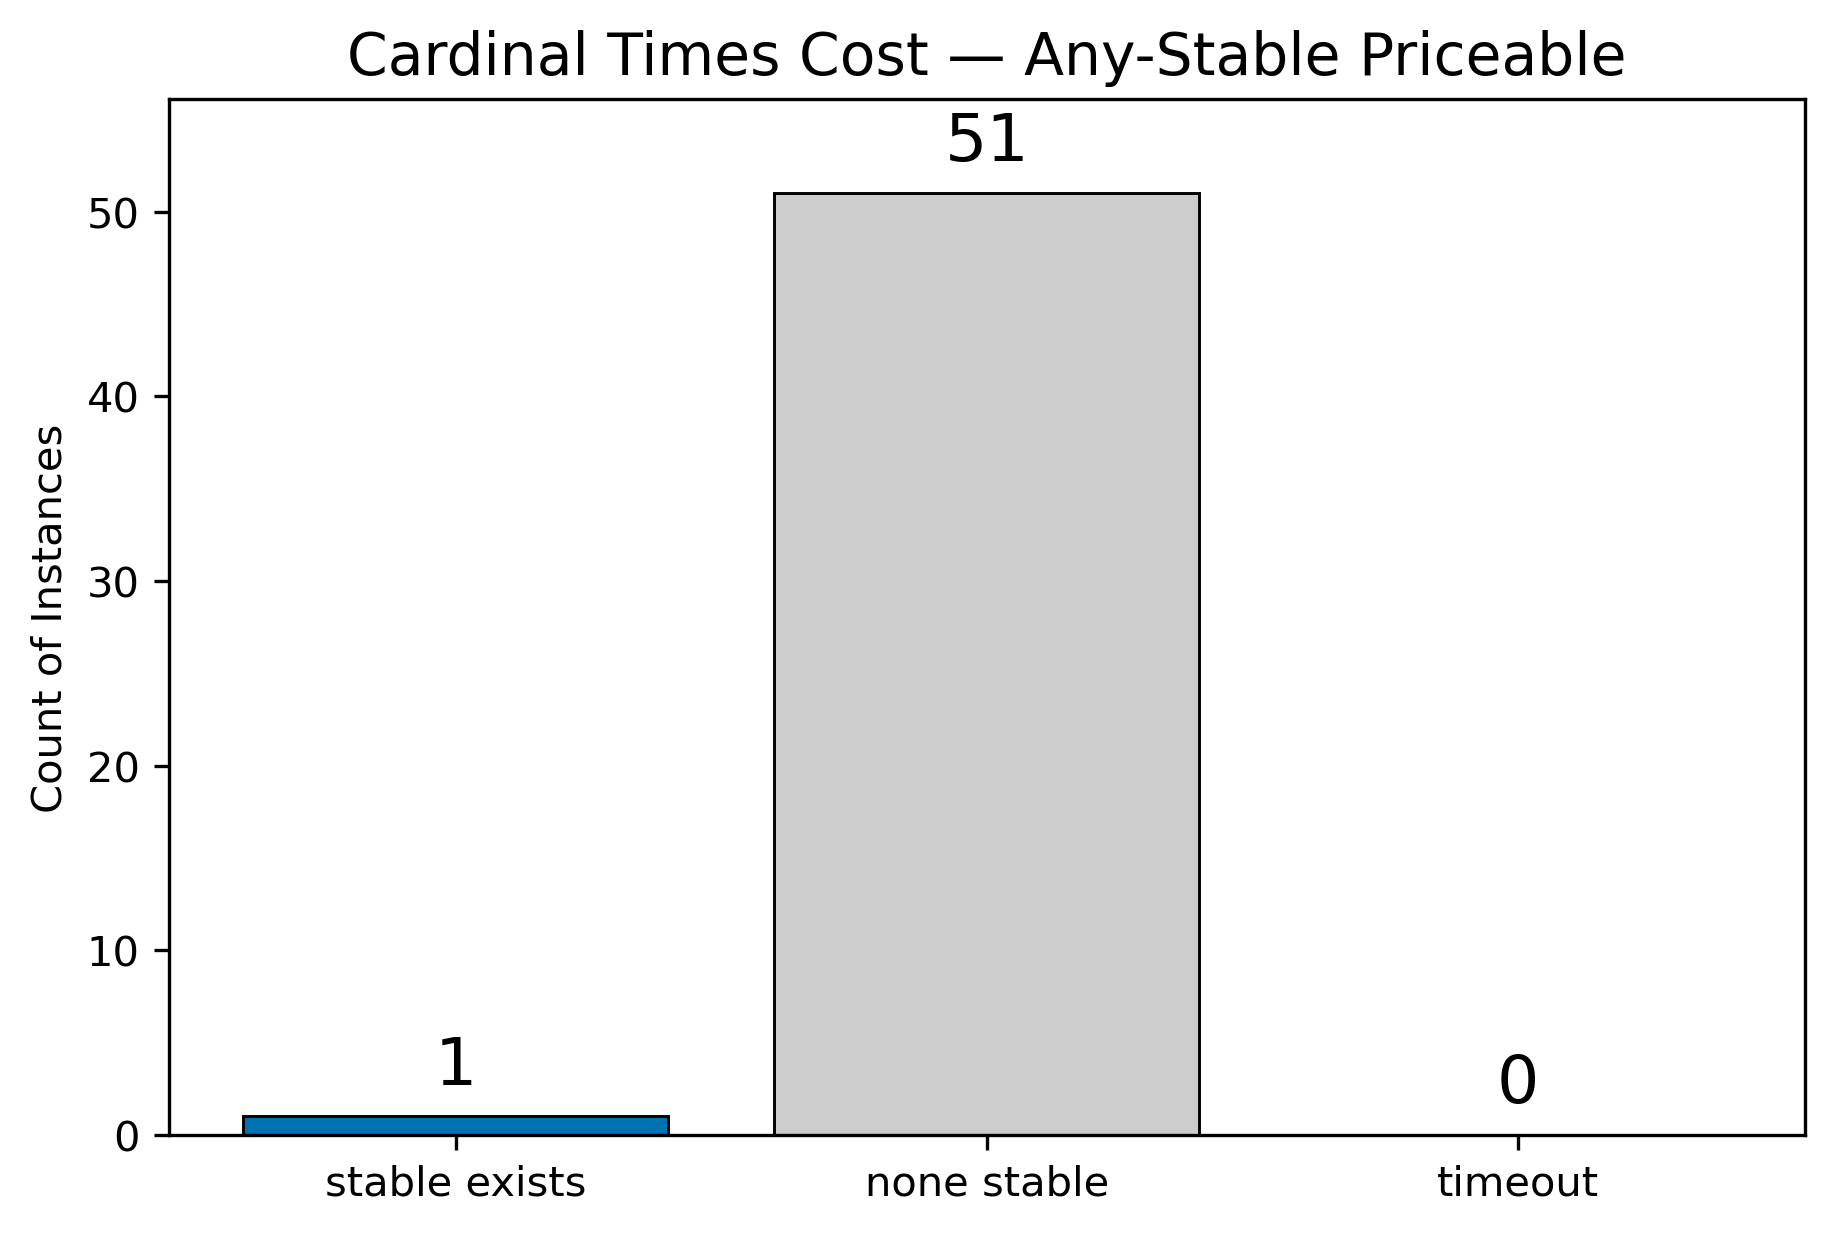
\includegraphics[width=0.7\textwidth]{figures/plots/cardinal-times-cost/cardinal_times_cost_any_stable_exhaustive.png}
  \caption{Number of instances, for which no method found exhaustive stable priceable solution, where such a solution exists or does not, for cardinal-based elections with cost utilities.}
  \label{fig:myplot}
\end{figure}
Similarly as for pure priceability, tested methods fail to find exhaustive stable priceable outcomes largely, because they do not exist. Again, that should be considered an acceptable result for proportionality provided by variations of MES, no matter the type of ballot or satisfaction measure.

\chapter{Conclusion}\label{chap:5}
The recently introduced market-based axioms for proportionality --- stable-priceability and priceability --- have proved to imply a high degree of proportionality. Adjusting them to be suitable for more precise voting methods was a natural step to take in studying fairness properties in Participatory Budgeting elections.


Extending the notion of stable priceability to account for cumulative profiles and, more generally, cardinal profiles allows for examining allocations and election rules in almost all instances of PB elections worldwide. Thanks to keeping its computational advantages over other axioms, such as the core, it will also make it possible to perform a quicker analysis of other traits of voting outcomes. The intuition behind the new definition is similar to original definition, therefore the implied fairness of the axiom holds. Moreover, we have defined and proved the most important properties of the newly defined stable priceability, namely
\begin{enumerate}
    \item it reduces to the original approval-based definition when working with binary utilities.
    \item it does not improve the core in the general case, but it does imply the core up-to-one.
    \item there exists an ILP program that can verify in polynomial time, given an election instance and an allocation, if that allocation is supported by a stable price system.
\end{enumerate}

Implementation of the algorithm for the new stable priceability definition in the open-source Pabutools library using state-of-the-art linear programming tools, alongside robust tests paves the way for further analysis of the defined properties by other researchers in the future. 

Our empirical evaluation on a diverse collection of real‐world participatory budgeting instances—from several dozen Polish and other European cities—confirms the practical relevance of our approach.  We ran each of the five rules (MES, MES+Inc, MES+BOS, UGreedy and the MES+Inc+UGreedy hybrid) on over $300$ historical ballots, measuring 
\begin{enumerate}
    \item the fraction of priceable and stable priceable outcomes under the standard and cost‐weighted utility models.
    \item the percentage of stable priceable outcomes, which are also exhaustive.
    \item the overall coverage of priceability and stable priceability exercised by the $4$ tested election rules.
    \item the fraction of elections, for which no method has found exhasutive priceable or stable priceable allocations, which do have such an allocation, and the fraction of elections, which do not have a single outcome satisfying those conditions.
\end{enumerate}
We observed that MES+Inc achieves the highest stable‐priceability rates (exceeding $90\%$ for cost-adjusted cases), and that combining it with the utilitarian greedy method recovers exhaustiveness without loss of stability in large majority of cases. Moreover, no single rule solved every instance perfectly, but the five‐rule portfolio provided perfect results for most of our dataset --- demonstrating both the strengths and complementarity of these methods in practice. 

Beyond evaluation of existing rules, our results suggest promising avenues for new or tweaked election methods specifically designed to maximise stable priceability, especially under exhaustiveness clause. Preliminary experiments with different versions of the Method of Equal Shares  have shown potential gains of several percentage points in exhaustive stability rates, indicating that further rule‐design tailored to the cost‐weighted setting could yield even stronger proportionality guarantees without sacrificing computational tractability.

Additionally, developing meaningful \emph{relaxations} of the formulation of SP under additive utilities is therefore a rich direction for future work. For instance, one could allow small “stability deficits” in exchange for greater exhaustiveness, or introduce budget‐slack parameters that flexibly trade off exact proportionality for practical implementability. Such relaxed variants could broaden the applicability of stable priceability to even more complex preference models and institutional constraints, while retaining its core normative appeal.  

\printbibliography[
    heading=bibintoc,
    title={Bibliography}
]


\end{document}


%%% Local Variables:
%%% mode: latex
%%% TeX-master: t
%%% coding: latin-2
%%% End: